%%% additional documentclass options:
%  [doublespacing]
%  [linenumbers]   - put the line numbers on margins

%%% loading packages, author definitions

%\documentclass[twocolumn]{bmcart}% uncomment this for twocolumn layout and comment line below
\documentclass{bmcart}
\usepackage[utf8]{inputenc}
\usepackage{amsmath}
\usepackage{amssymb}
\usepackage{graphicx}
\usepackage[font=scriptsize,labelfont={bf}]{caption}
\usepackage[justification=raggedright,nearskip=10pt,farskip=0pt]{subfig}
\usepackage{calc}
\usepackage{url}
\usepackage{array}
\usepackage{rotating}
\usepackage{tabularx}
\usepackage{multirow}
\usepackage{layouts}
\usepackage{titletoc}
\usepackage{setspace}
\usepackage{longtable}
\usepackage{pgf}
\usepackage{tikz}
\usetikzlibrary{shapes,arrows}
\usepackage{footnote}

%%%%%%%%%%%%%%%%%%%%%%%%%%%%%%%%%%%%%%%%%%%%%%%%%
%%                                             %%
%%  If you wish to display your graphics for   %%
%%  your own use using includegraphic or       %%
%%  includegraphics, then comment out the      %%
%%  following two lines of code.               %%
%%  NB: These line *must* be included when     %%
%%  submitting to BMC.                         %%
%%  All figure files must be submitted as      %%
%%  separate graphics through the BMC          %%
%%  submission process, not included in the    %%
%%  submitted article.                         %%
%%                                             %%
%%%%%%%%%%%%%%%%%%%%%%%%%%%%%%%%%%%%%%%%%%%%%%%%%
% \def\includegraphic[#1]#2{}
% \def\includegraphics[#1]#2{}

%%% Put your definitions there:
\startlocaldefs
\hbadness=9999999 %avoid complaining for underfull h/vbox
\vbadness=9999999

% \setlength{\columnwidth}{86mm}
 \captionsetup[subfloat]{labelformat=empty} %position=top, justification=raggedright, singlelinecheck=false, labelformat=simple, font={scriptsize,sf,bf}, width=0.5\textwidth}
 \captionsetup{width=0.95\textwidth, indention=-12pt}
 \renewcommand*\thesubfigure{\Alph{subfigure}}
 \setlength{\belowcaptionskip}{-3mm}
 %\setlength{\abovecaptionskip}{0mm}
%\addtolength{\abovecaptionskip}{-3mm}

%\subfiguretopcaptrue

\pdfminorversion=4
\pdfobjcompresslevel=0

\pgfdeclareimage[height=3ex]{win-logo}{images/win_logo}
\pgfdeclareimage[height=3ex]{mac-logo}{images/mac_logo}
\pgfdeclareimage[height=3ex]{linux-logo}{images/linux_logo}
\pgfdeclareimage[height=3ex]{ubuntu-logo}{images/ubuntu_logo}
\pgfdeclareimage[height=2ex]{mac-command}{images/mac_command}
\pgfdeclareimage[height=2ex]{lower-bound}{images/lowerbound}
\pgfdeclareimage[height=2ex]{upper-bound}{images/upperbound_green}

\newcommand{\winsymbol}{\raisebox{-0.8ex}{\pgfuseimage{win-logo}}}
\newcommand{\macsymbol}{\raisebox{-0.5ex}{\pgfuseimage{mac-logo}}}
\newcommand{\linuxsymbol}{\raisebox{-0.8ex}{\pgfuseimage{linux-logo}}}
\newcommand{\ubuntusymbol}{\raisebox{-0.9ex}{\pgfuseimage{ubuntu-logo}}}
\newcommand{\winmaclinux}[3]{\begin{itemize}
    \item[\winsymbol] #1
    \item[\macsymbol] #2
    \item[\linuxsymbol] #3
\end{itemize}}
\newcommand{\macpc}[2]{\begin{itemize}
    \item[\macsymbol] #1
    \item[\winsymbol\ \  \linuxsymbol] #2
\end{itemize}}

\newcommand{\maccmd}{\raisebox{-0.35ex}{\pgfuseimage{mac-command}}}

\setlength{\abovecaptionskip}{1.3mm}
%\setlength{\belowcaptionskip}{1mm}

\def\ta{Timed Automaton}
\def\tas{Timed Automata}
\def\animo2{ANIMO 2}

%\setvaluelist{bmcsymbol}{*,\textdagger,\^{}}
\def\textdagger{\#{}} %I would be very happy to avoid the distasteful symbol \textdagger (or \dagger, whatever).

%\def \doiurl#1{\textsf{#1}}

\endlocaldefs

\makeindex

\begin{document}

\begin{frontmatter}

\begin{fmbox}
\dochead{Methodology}

\title{Modelling with ANIMO:\\ between Fuzzy Logic and ODE}%ODE vs Fuzzy Logic: in medio stat ANIMO}%Formal models of biological networks in \animo2{}} %Building formal models of biological networks avoiding formal training}

%%%%%%%%%%%%%%%%%%%%%%%%%%%%%%%%%%%%%%%%%%%%%%
%%                                          %%
%% Enter the authors here                   %%
%%                                          %%
%% Specify information, if available,       %%
%% in the form:                             %%
%%   <key>={<id1>,<id2>}                    %%
%%   <key>=                                 %%
%% Comment or delete the keys which are     %%
%% not used. Repeat \author command as much %%
%% as required.                             %%
%%                                          %%
%%%%%%%%%%%%%%%%%%%%%%%%%%%%%%%%%%%%%%%%%%%%%%

\author[
   addressref={aff1},                   % id's of addresses, e.g. {aff1,aff2}
   %corref={aff1},                       % id of corresponding address, if any
   noteref={n1},                        % id's of article notes, if any
   email={s.schivo@utwente.nl}   % email address
]{\inits{S}\fnm{Stefano} \snm{Schivo}}
\author[
   addressref={aff2},
   noteref={n1},
   email={j.scholma@utwente.nl}
]{\inits{J}\fnm{Jetse} \snm{Scholma}}
% \author[
%    addressref={aff3},
%    email={b.wanders@utwente.nl}
% ]{\inits{B}\fnm{Brend} \snm{Wanders}}
% \author[
%    addressref={aff2},
%    email={rauc6788@hotmail.com}
% ]{\inits{RA}\fnm{Ricardo A.} \snm{Urquidi Camacho}}
\author[
   addressref={aff3},
   email={p.e.vandervet@utwente.nl}
]{\inits{PE}\fnm{Paul E.} \snm{van~der~Vet}}
\author[
   addressref={aff2},
   email={h.b.j.karperien@utwente.nl}
]{\inits{M}\fnm{Marcel} \snm{Karperien}}
\author[
   addressref={aff2},
   %corref={aff2},
   email={j.n.post@utwente.nl}
]{\inits{JN}\fnm{Janine N.} \snm{Post}}
\author[
   addressref={aff1},
   %corref={aff1},
   email={j.c.vandepol@utwente.nl}
]{\inits{J}\fnm{Jaco} \snm{van~de~Pol}}
\author[
   addressref={aff1},
   corref={aff1},
   email={r.langerak@utwente.nl}
]{\inits{R}\fnm{Rom} \snm{Langerak}}

%%%%%%%%%%%%%%%%%%%%%%%%%%%%%%%%%%%%%%%%%%%%%%
%%                                          %%
%% Enter the authors' addresses here        %%
%%                                          %%
%% Repeat \address commands as much as      %%
%% required.                                %%
%%                                          %%
%%%%%%%%%%%%%%%%%%%%%%%%%%%%%%%%%%%%%%%%%%%%%%

\address[id=aff1]{%                           % unique id
  \orgname{Formal Methods and Tools, Faculty of EEMCS, University of Twente}, % university, etc
  %\street{Hallenweg},                     %
  \postcode{7522NH}                           % post or zip code
  \city{Enschede},                              % city
  \cny{The~Netherlands}                                    % country
}
\address[id=aff2]{%
  \orgname{Developmental BioEngineering, MIRA Institute for Biomedical Technology and Technical Medicine, University of Twente},
  %\street{ },
  \postcode{7522NH}
  \city{Enschede},
  \cny{The~Netherlands}
}
\address[id=aff3]{%
  \orgname{Human Media Interaction, Faculty of EEMCS, University of Twente},
  %\street{ },
  \postcode{7522NH}
  \city{Enschede},
  \cny{The~Netherlands}
}

%%%%%%%%%%%%%%%%%%%%%%%%%%%%%%%%%%%%%%%%%%%%%%
%%                                          %%
%% Enter short notes here                   %%
%%                                          %%
%% Short notes will be after addresses      %%
%% on first page.                           %%
%%                                          %%
%%%%%%%%%%%%%%%%%%%%%%%%%%%%%%%%%%%%%%%%%%%%%%

\begin{artnotes}
%\note{Sample of title note}     % note to the article
\note[id=n1]{Equal contributor} % note, connected to author
\end{artnotes}
% 
% \let\oldthefootnote\thefootnote
% \renewcommand{\thefootnote}{\fnsymbol{footnote}}
% \footnotetext[1]{These authors contributed equally to this work.}
% \footnotetext[3]{To whom correspondence should be addressed.}
% \let\thefootnote\oldthefootnote


\end{fmbox}% comment this for two column layout


\maketitle

%%%%%%%%%%%%%%%%%%%%%%%%%%%%%%%%%%%%%%%%%%%%%%
%%                                          %%
%% The Abstract begins here                 %%
%%                                          %%
%% Please refer to the Instructions for     %%
%% authors on http://www.biomedcentral.com  %%
%% and include the section headings         %%
%% accordingly for your article type.       %%
%%                                          %%
%%%%%%%%%%%%%%%%%%%%%%%%%%%%%%%%%%%%%%%%%%%%%%

\begin{abstractbox}

\begin{abstract} % abstract <= 350 words. Headers: background, results, conclusions
\parttitle{Background}
The large amount of data which an experimental biologist
must deal with makes it nearly impossible to reason on
the dynamics of complex systems without relying on computational
support.
The software tool ANIMO (Analysis of Networks with Interactive MOdelling)
provides such computational support to the experimental biologist.
Models built with ANIMO allow to reason about the complex networks of signaling events
occurring in living cells.
The user-friendly interface allows biology experts to exploit formal methods
without the need to become experts also in mathematical formalisms.
\parttitle{Results}
ANIMO allows for a model precision that is intermediate between ordinary differential equations (ODEs)
and fuzzy logic.
We show this by presenting ANIMO models for two case studies: \emph{Drosophila melanogaster} circadian clock, and signal
transduction events downstream of TNF$\alpha$ and EGF in HT-29 human
colon carcinoma cells.
The models were originally developed with ODEs and
fuzzy logic respectively.
\parttitle{Conclusions}
% The software tool ANIMO, recently updated to work with the latest version of Cytoscape,
% allows the biologist to develop a formal model through a user friendly interface,
% achieving useful insight without the need to study any mathematical formalism.
%
ANIMO models allow to replicate with good precision the results of both the ODE and
fuzzy logic model. Moreover, ANIMO models require less parameters than ODEs and are more precise than
fuzzy logic: for this reason, we position the modelling paradigm of ANIMO
between ODEs and fuzzy logic.
\end{abstract}

%%%%%%%%%%%%%%%%%%%%%%%%%%%%%%%%%%%%%%%%%%%%%%
%%                                          %%
%% The keywords begin here                  %%
%%                                          %%
%% Put each keyword in separate \kwd{}.     %%
%%                                          %%
%%%%%%%%%%%%%%%%%%%%%%%%%%%%%%%%%%%%%%%%%%%%%%

\begin{keyword}
\kwd{modelling}
\kwd{signalling pathway}
\kwd{timed automata}
\kwd{dynamic behaviour}
\end{keyword}

% MSC classifications codes, if any
%\begin{keyword}[class=AMS]
%\kwd[Primary ]{}
%\kwd{}
%\kwd[; secondary ]{}
%\end{keyword}

\end{abstractbox}
%
%\end{fmbox}% uncomment this for twcolumn layout

\end{frontmatter}


\section*{Background}\label{sec:introduction}
\subsection*{Modelling in cell biology}


Executable biology is a young subfield in computational modeling, aimed at constructing models that mimic
biological phenomena \emph{in silico}. It provides an interesting paradigm for enhancing network
diagrams with an underlying formal description of both network components and their interactions.
Executable models typically contain a description of the direct interactions of network components,
requiring the modeler to think in terms of
``cause and effect''. Biologists reason in similar ways about the molecular mechanisms of network
interactions, and this makes construction of an executable model an intuitive process.
ANIMO (Analysis of Networks with Interactive MOdeling,~\cite{animo-ieee,animo-gene})
provides an enabling technology to increase the use of computational models by experimental
 biologists without a thorough mathematical background. Such models are indispensable for formally
comparing experimental data to prior knowledge, or for structuring experimental findings into a
new theory.
When dealing with complex biological networks, executable biology models are particularly useful
to understand the non-linear dynamics and the entailed emergent properties of the networks.
In those cases, an ANIMO model can be used as a support to obtain insight based on abstract
representations of the interactions occurring inside living cells.
Other applications of ANIMO models include performing \emph{in silico} experiments and
the storage and transfer of knowledge on biological networks.



% 
% In living cells, processes are regulated by networks of interacting molecules.
% Aberrations in these networks underlie a wide range of pathologies. The development of new therapies
% requires a thorough insight in the functioning of these networks. Obtaining such insight can be a challenging task.
% Feedback loops and crosstalk between pathways lead to an intricate wiring of the network.
% % Hence, it is necessary to study the ensemble of molecules involved, because the 
% % behaviour of individual molecules is not sufficient for a complete understanding. 
% Since the human brain is ill-suited to grasp the non-linear dynamics of these complex networks and
% the entailed emergent properties, the role of computational support is increasing
% in molecular biology.
% % 
% % 
% %
% % The systems biology approach to understanding biological systems starts off from a
% % scientific question and then follows an empirical cycle \--\ or rather a positive spiral \--\ of
% % knowledge/theory $\rightarrow$ model $\rightarrow$ hypotheses $\rightarrow$ experiments $\rightarrow$
% % observations $\rightarrow$ update and/or refinement of knowledge/theory,
% % until an answer to the original question is found (Figure~\ref{fig:empirical-spiral}).
% In this context, we can profit from models in different ways:
% \begin{enumerate}
%   \item to organize data and store knowledge,
%   \item to structure reasoning and discussion
%   \item to perform \emph{in silico} experiments and derive hypotheses.
% \end{enumerate}
% % An \emph{in silico} model is always a simplified representation of biological reality and is never the 
% % aim in itself.
% % Rather, it is a powerful means in the process of gaining an understanding of the biological system.
% % Given its role in the empirical cycle, the process of modelling is especially effective
% % when applied by the experts with respect to a certain biological system. Biologists usually have a good sense 
% % of cause-and-effect relationships of molecular interactions. In addition, they are the most knowledgeable
% % on the network topology and the dynamics of the biological system they are studying.
% % Since they also benefit most from the generation of hypotheses and from an efficient experimental design, 
% % biologists would be the primary candidates to construct models of their research topic.
% 
% 
% As models are a formalization of knowledge or theories, an underlying formalism is needed to express
% this knowledge. Different formal methods have been successfully applied to construct representations
% of biological systems. Among these methods are Boolean logic~\cite{boolean-networks,boolean-networks-flower,boolean-networks2},
% ordinary differential equations (ODEs, reviewed in~\cite{hidde-review}),
% interacting state machines~\cite{interacting-sm1,interacting-sm2},
% process calculi~\cite{regev-shapiro,blenx,bio-pepa}, Timed Automata~\cite{ta-siebert,bartocci-oscillators,
% oded-ode-ta-discretization} and Petri nets~\cite{petri-nets0,petri-nets,petri-nets2}.
% Most of these formal methods have been implemented into software tools to aid the process
% of modelling. Due to the lack of such a supporting tool, \tas\ have remained a less 
% frequently applied method.

% \subsection*{\tas\ for biological models}
% \tas\ have been developed to model the dynamic behaviour of systems with processes running in parallel~\cite{timed-automata-alur-dill}. 
% As such, \tas\ have been applied in communication protocols and industrial control engineering~\cite{ta-audio-protocol,ta-wap-gateway,ta-ws-bap}. The 
% parallels between these application areas and regulatory processes in cells have triggered the step towards 
% their use in biology.
% In~\cite{ta-siebert}, the authors used \tas\ to extend a classical modelling paradigm~\cite{thomas-formalism},
% allowing to add temporal dynamics to gene network models.
% In~\cite{bartocci-oscillators}, a model of biological oscillators was described and synchronization properties
% were tested in this dynamic system.
% A discretization of ODEs to \tas\ was proposed in~\cite{oded-ode-ta-discretization}, applying
% a translation between the two formalisms to an example gene regulatory network. Two 
% different approaches to transforming
% a Petri net model into \tas\ were presented in~\cite{ta-giapponesi},
% where the important issue of state space explosion was also addressed.
% Finally, the authors of~\cite{ta-radiazioni} proposed an \emph{ad hoc} \tas\ model of a radiation treatment
% system, which was then validated through the analysis tool UPPAAL~\cite{uppaal}.\\
% Each of these approaches has been successfully validated, demonstrating the potential of \tas\
% in biological applications. However, these approaches were all limited to simple
% or specific examples and none of these modelling methods
% has led to a tool implementation of the proposed method to encourage a broader use
% of \tas\ in molecular biology. We have recently introduced the software tool ANIMO
% (Analysis of Networks with Interactive MOdelling,~\cite{animo-ieee}), which aims
% at making available the power of \tas\ to the experimental biologists without requiring
% them to be fluent in any mathematical formalism.
% 
% % Mastery of most existing modelling tools requires training and experience in mathematical modelling. 
% % In this respect, a lack of tradition in quantitative
% % reasoning and formal methods within the biological community at large is still a stumbling block for
% % widespread application of modelling of biological systems. Here, we present an intuitive method for the
% % construction of formal in silico models of the dynamics of molecular networks, supported by a novel,
% % user friendly modelling tool, ANIMO (Analysis of Networks with Interactive 
% % MOdelling,~\cite{animo-ieee}). \tas\ are used as the underlying mathematical formalism.
% 
% % In the Methods section, we will explain how choosing a suitable abstraction level can make the construction
% % of models more intuitive. We will then show how ANIMO is designed to support the modelling process following
% % this approach. Construction of a small model based on experimental data will exemplify the method that we
% % propose. In the Results section, we first show an ANIMO model of the genes and proteins that constitute
% % the circadian clock network in \emph{Drosophila Melanogaster}. The remainder of that section is dedicated to
% % illustrate how a single modelling iteration in the empirical cycle is used to compile prior knowledge and
% % experimental data into a model, perform \emph{in silico} simulations and derive meaningful testable 
% % hypotheses. These hypotheses are supported by literature on interactions in different cell types.
% 
% In this paper we present \animo2{}, an updated version of ANIMO which allows for a considerably
% more efficient analysis of models. \animo2{} also introduces new features, such as the possibility to interrogate
% an ANIMO model with model checking queries represented as human language sentences instead of
% mathematical formulae. The case studies presented in this paper are centered around possible usage scenarios
% for ANIMO, and aim at illustrating how a biologist can profit from the tool in its latest iteration.
% An installation and user manual for \animo2{} is available at \url{http://fmt.cs.utwente.nl/tools/animo/manual.html}.

% \subsection*{A short introduction to ANIMO}
% {\Large [[briefly describe ANIMO, its modelling assumptions and its intended use. Refer to Gene paper?]]}



\section*{Results}\label{sec:results}
\subsection*{Modelling oscillation}\label{sec:animo-drosophila}
Results obtained with ANIMO are comparable to results with other modeling
approaches. To demonstrate this, Figure~\ref{fig:drosophila-model}
represents an ANIMO model of the circadian clock in \emph{Drosophila Melanogaster}, based on~\cite{drosophila-ode-model},
where ordinary differential equations (ODEs) were used.
The cyclic behavior of the circadian clock is based on the alternating formation and destruction of the
CYC/CLK protein complex.
Concentration levels of this complex are in turn regulated by a series of proteins which are produced as
a consequence of CYC/CLK formation. The CWO protein
is central to the functioning of the network, as it degrades the mRNA for most of the involved proteins.
As such, CWO acts as an inhibitor that counterbalances the effect of CYC/CLK.
The positive influence of the light-regulated cryptochrome CRY on the degradation of TIM is a consequence
of the passage between day and night, allowing
the circadian clock to synchronize to a time zone (see Suppl. Sect.~\ref{suppl:repressilator}).




The output of the ANIMO model in Figure~\ref{fig:drosophila-model} closely matches the original ODE model.
In particular, the oscillations in both models show the same periods and phases (see Suppl. Fig~\ref{suppl-fig:grafici-drosophila}).
% Due to the compositional nature of \tas\, ANIMO allows for intuitive \emph{in silico} knock-out experiments,
% by right-clicking a node in the model and disabling it. Such experiments have been done
% before~\cite{drosophila-ode-model} and give similar results in our model.
Details of the comparison
between the ANIMO model and the original ODE model is given in Supplementary Section~\ref{suppl-sec:animo-drosophila}.
% \\
% {\Large [[Insert description of K.O. experiments with Drosophila model]]}




\subsection*{Using ANIMO to generate hypotheses}\label{subsec:case-study-larger}
We constructed a model of the signaling network downstream of TNF$\alpha$ and EGF, formalizing
the crosstalk that takes place between the pathways at different levels of cellular regulation.
We first modeled the two pathways in isolation~(Suppl. Figs.~\ref{fig:large-model-tnf}, \ref{fig:large-model-egf}),
using information on protein interactions from
the KEGG~\cite{kegg} and phosphosite~\cite{phosphosite} databases. These models were fitted to experimental data
from previous studies~\cite{pathway-compendium,pathway-autocrine}.
We then merged the two pathways into a single model and added autocrine crosstalk between the pathways that has been
described in~\cite{pathway-autocrine}.
Briefly, stimulation with TNF$\alpha$ ({\sf TNFa} in the model) leads to a rapid release of TGF$\alpha$ ({\sf TGFa}),
which activates the EGF receptor ({\sf EGFR}).
This activation causes secretion of IL-1$\alpha$ ({\sf IL-1a}) at later time points.
The effect of IL-1$\alpha$ is down-regulated by the secretion of IL-1 receptor antagonist ({\sf IL-1ra})
downstream of TNF$\alpha$.
The resulting model (Fig.~\ref{fig:large-model-no-hypotheses}) was compared to the experimental data
for treatments with 100 ng/ml TNF alone and 100 ng/ml EGF alone (data not shown)~\cite{pathway-compendium}.

At this point, the behavior of the model deviated from the data for some of the nodes.
Changing the parameters of the model was not enough to reproduce the behaviour shown by experimental
data. This is an interesting situation, as it requires changes in the topology of
the model, which can be interpreted as new hypotheses. Below, we give two examples and show how
adaptation of the model can be used to generate novel testable hypotheses.





Experimentally,
treatment with TGF$\alpha$ alone does not lead to secretion of IL-1$\alpha$. Instead, a co-stimulation with
TGF$\alpha$ and TNF$\alpha$ is required~\cite{pathway-autocrine}.
However, in the first version of the model, treatment with TGF$\alpha$ was sufficient for
IL-1$\alpha$ expression (Fig.~\ref{fig:large-model-graph1}). Given the time delay until secretion of IL-1$\alpha$, it can be
expected that \emph{de novo} synthesis of IL-1$\alpha$ is required and that both
TNF$\alpha$ and TGF$\alpha$ are needed to activate transcription of the IL-1$\alpha$ gene.
JNK1 and ERK signal downstream of TNF$\alpha$ and TGF$\alpha$, respectively, and are known
to affect the activity of multiple transcription factors. We altered the model to make
activation of IL-1$\alpha$ expression dependent on both JNK1 activity and ERK activity
(Suppl. Fig.~\ref{fig:large-model-hypotheses}, arrows linking {\sf JNK1} and {\sf ERK} to {\sf IL-1a gene}).
After this modification to the model, IL-1$\alpha$ was no longer secreted
upon stimulation with TGF$\alpha$ alone, which greatly improved the fit between the measured IL-1$\alpha$
levels and the model (Fig.~\ref{fig:large-model-graph2}). This hypothesis could now be used to
design a new experiment to validate IL-1$\alpha$ as a target of combined JNK1 activity and ERK activity in
HT-29 cells. For example, kinase inhibitors specific to JNK1 and ERK could be used to confirm that activity of
both kinases is required for expression and secretion of IL-1$\alpha$. Performing the experiment is beyond
the scope of this study, but this hypothesis finds support in literature.
Transcription factors c-Jun and c-Fos together
form a heterodimer known as AP-1 and are activated by JNK1 and ERK,
respectively~\cite{jnk-signaling,cfos-cjun}. AP-1 has been reported to bind to the
promoter of IL-1$\alpha$, providing evidence for a role in the regulation of IL-1$\alpha$
expression~\cite{ap1-il1a}. Based on these findings in literature we included c-Jun and
c-Fos in our model as transcriptional activators of IL-1$\alpha$ (Fig.\ref{fig:large-model-complete}).



As a second example, we considered the behaviour of JNK1 and MK2. In the model, both
proteins were located downstream of TNF$\alpha$ but not TGF$\alpha$ or EGF. Hence, the
model did not show an effect of C225, a pharmacological inhibitor of ligand-EGFR
binding, on activation of JNK1 or MK2 after stimulation with TNF$\alpha$. However, experimental
data show that C225 strongly reduces activation of JNK1 and MK2 upon stimulation with
TNF$\alpha$~\cite{pathway-autocrine}.
This fact is indicative of a role for EGFR in activation of JNK1 and MK2. Since both JNK1 and MK2
are located downstream of MEKK1, we hypothesized that activation
of MEKK1 is dependent on
both TNF$\alpha$-signalling and TGF$\alpha$-signalling. In the model we added a new
hypothetical node {\sf Hyp~2} (hypothesis~2) to link EGFR to MEKK1 (Suppl. Fig.~\ref{fig:large-model-hypotheses}).
This addition led to an improved fit of the model to the data upon treatment with TNF$\alpha$ + C225:
activation of both MK2 and JNK1 was strongly suppressed by C225 (Fig.~\ref{fig:large-model-graph4}).
Stimulation with EGF alone did not lead to activation of JNK1 and MK2.
These data support the validity of the modification to the model.
Further support for a link between EGFR and MEKK1 was found in literature. Specifically,
Ras has been reported as a direct activator of
MEKK1~\cite{ras-mekk1}. EGFR is a well-known and potent activator of Ras,
which is why it was already in our network~\cite{kegg}.
Other studies also report activation of JNK1 and phosphorylation of c-Jun downstream of Ras, which is consistent with
an interaction between Ras and MEKK1~\cite{cfos-cjun,ras-jnk1}.
Based on these findings, we adapted
our model by removing the {\sf Hyp~2} node and creating a direct interaction between Ras
and MEKK1 (Fig.~\ref{fig:large-model-complete}). Experimentally, the role of Ras could be confirmed by using a
pharmacological inhibitor of Ras activity, and measuring the effect of this inhibitor on the activation of JNK1 and MK2.
Together, our model suggests that EGFR activity is required
but not sufficient for activation of JNK1 and MK2 in HT-29 cells.


There are other nodes for which the experimental data deviates from the model in one or more of the experimental conditions.
A comparison between model and experimental data can be found in Figures~\ref{fig:differences1}, \ref{fig:differences2} and~\ref{fig:differences3}.
A complete deciphering of the signalling events
in this biological system is outside the scope of this paper. Instead, we illustrated how interactive modelling of the dynamic behaviour
of a signal transduction network can be used to extend previous pathway topologies and can lead to the generation of novel hypotheses.







\section*{Discussion}
\subsection*{Final remarks on the models}
In the Results section, we described the construction of an ANIMO
model of the circadian clock in \emph{Drosophila Melanogaster}. This model
captured the dynamics of the regulatory network and led to similar 
conclusions as an ODE model that had been
published previously~\cite{drosophila-ode-model}. This finding supports the use of
the series of modeling abstractions on which ANIMO is based. The biggest
difference between the construction of these models is that the model in~\cite{drosophila-ode-model}
is constructed by writing a system of mathematical equations, together
with an algorithm for simulation. In ANIMO, instead, a number of network
nodes is drawn for the molecules involved. 
These nodes are then linked by directed
interactions that represent cause-and-effect relationships, with a single parameter 
that defines the strength of each
interaction. This is a more intuitive approach to construct a model.
Further contributing to an interactive modeling process
is the compositionality of the model. Each node in the network
can be disabled at any time by the user, or extra nodes can be added,
without having to change any of the existing interactions.

In the Results section we also showed the construction of an executable model
of signaling events downstream of
TNF$\alpha$ and EGF in human colon carcinoma cells. This data set has been used for
previous modeling studies, based on partial least-squares regression and fuzzy 
logic~\cite{pathway-leastsquare,pathway-fuzzy}.
The partial least-squares regression model describes an abstract data-driven model 
that uses statistical correlations
to relate signal transduction events to various cellular decisions. This type of modeling is
very useful in uncovering new and unexpected relations. It is also successful in making
predictions, but gives little direct in the dynamic behavior of the network. Fuzzy
logic analysis led to a model that gave a better fit to the dynamic network behavior than
discrete logic (Boolean) models. Inspection of the inputs to the logical gates that were used
to model protein behavior led to the prediction of novel interactions between proteins,
showing the usefulness of this approach. For most of the proteins, such as JNK1, time was
used as an input parameter. For example, the logical gates ``if TNF$\alpha$ is high
\emph{AND} time is low, then JNK1 is high'' and ``if TNF$\alpha$ is high \emph{AND} time is
high, then JNK1 is low'' were used to
describe the dynamic behavior of JNK1. Although this leads to a representative
description of the dynamic behavior of JNK1, peaks in protein activity at early time points were
not reproduced by the fuzzy logic model. Moreover, it gives no insight in the molecular interactions 
that are involved in activation or inhibition.

In this study, we used a data set based on the experiments described in~\cite{pathway-compendium}. We used the
resulting experimental data, together with knowledge from curated databases~\cite{kegg,phosphosite}
to construct an executable model of the biological system.
In contrast with the two approaches described above, ANIMO is aimed at the construction of
more mechanistic models, mimicking biochemical interactions \emph{in silico}. This way of modeling
gives a different type of insight. In the process of model construction, we extended a
prior-knowledge network with time-dependent extracellular crosstalk that has been reported
previously~\cite{pathway-autocrine}. To come up with possible explanations for a disagreement
between the model and the experimental data, two additional layers of
crosstalk were introduced, at the signal transduction and transcriptional level. These modifications 
improved the fit of the model to the data and can be interpreted as novel testable hypotheses.
Finally, we proposed new experiments that could be carried out to test these hypotheses, closing the empirical cycle. 
Together, our model sheds more light on the intricate
entanglement between the TNF$\alpha$ and EGF pathways at multiple cellular levels.
But above all,  the model provides an excellent starting point for further investigation.
% Every new round in the empirical cycle will lift the understanding of the system to a higher level,
% leading to an incremental build-up of knowledge and an upward empirical spiral. Being intuitively
% accessible, ANIMO models facilitate sharing knowledge within and between groups and encourage collaborations.


\subsection*{Comparison between ANIMO and other modeling tools}\label{suppl:comparison-table}
Different formalisms are in use in the field of computational
modeling of biological systems, each with their specific characteristics.
Many of these formalisms have been implemented into
software tools to support modeling efforts. In order to compare
ANIMO with existing tools, we have selected a number of mathematical formalisms,
each connected to a supporting tool. With an emphasis on the modeling
process rather than the final model, we compared these tools on
the basis of the following parameters:

\begin{enumerate}
  \item {\bf Hidden formalism:} a knowledge of the underlying formalism is not required in order to use the tool
  \item {\bf Visual modeling:} the tool allows the user to model using a visual interface, and is not exclusively
      founded on formula-, text- or table-based input forms
  \item {\bf Qualitative parameters:} parameters for reactions can be input as approximated estimations, and not exclusively as numbers
  \item {\bf Tight coupling with topology:} models are tightly and clearly coupled to the networks they represent, showing the visual
      representation of the model in a shape similar or comparable to the representation currently used by biologists
      for signaling pathways
  \item {\bf User-chosen granularity:} if discretization is applied during the modeling process, the user can change the granularity
      with which such discretization is made, possibly for each component of the model separately
\end{enumerate}
Table~\ref{tab:tool-comparison} shows the comparison between ANIMO and the selected tools.

Going beyond the user interface, there are a number of ``pros and cons'' for using ANIMO and \tas\ 
in the biological context. First and foremost, being \tas\ an executable formal language,
a state space can be derived from a \tas\ model. This means that state space-related analyses
such as model checking can be performed on \tas: as explained in the Results section, this can
be done directly in ANIMO, bypassing the need for a deeper understanding of \tas\ as
ANIMO acts as an intermediary towards the powerful model checking tool UPPAAL.

The smaller amount of parameters needed to build an ANIMO model, if compared e.g. to
a differential equation-based approach, makes the modeling process faster, allowing
the biologist to obtain interesting results in less time. However, a less
parameter-intensive modeling approach is also less precise: in our case we abstract
sequences of biochemical reactions into activation or inactivation interactions,
simplifying any relation between two entities in a network as either activating or
inhibiting. While this allows for some simplifications in the networks and the underlying
formal models, it does not allow to represent in full detail more specific concepts
such as reactant concentration or reaction affinity. In case such concepts are of
primary importance, we encourage the interested reader to turn to more precise
modeling approaches, such as those based on differential equations.

All reactants modeled in ANIMO are assumed to be present at the same
(unitary) concentration. While this assumption is not always applicable, it encourages
abstract thought: many biological processes can be represented as networks driven by
\emph{activity-based} interactions. Even if with a limited scope, ANIMO can be applied
also in the analysis of metabolic processes, considering the production of protein $A$ as
the activation of node $A$, with degradation being represented as inhibition. As stated before,
it cannot be expected from such models to be a completely realistic representation of their target biological
processes, but they can still be an useful tool. This can be seen for example in the Drosophila
model in the Results section, where mRNA and protein concentrations were abstracted to
activity-driven processes in the ANIMO model.





\section*{Conclusions}
% The ultimate aim of research projects is to solve a problem or get
% the answer to a scientific question. In biology, an in-depth understanding of
% the relevant biological system is an important step towards this goal. Successive 
% repetitions of the empirical cycle result in a stepwise increase in understanding,
% until the goal is reached. For complex biological systems, computational modelling is 
% indispensable in this process. The mere act of creating 
% a computational model based on prior knowledge, experimental data and hypotheses 
% assists in gaining more insight in the system. 
% 
% %Furthermore, \emph{in silico} experiments 
% %with the model can be used to make predictions that cannot be made by the human brain. 
% 
% We developed a new modelling approach by proposing a series of abstractions from the detailed 
% molecular mechanisms of biological systems. These abstractions reduce the need for kinetic 
% parameters, while preserving enough expressivity for a useful description of the dynamic 
% behaviour of biological networks. A novel modelling tool, ANIMO, allows 
% effective use of this approach and enables an intuitive construction of formal models.

ANIMO is not the first modeling tool to provide an interface to a
modeling formalism. Such interfaces exist in many other tools (as shown in Tab.~\ref{tab:tool-comparison}). With its
focus on user-friendliness and intuitive modeling, ANIMO's main contribution lies 
in making computational modeling more accessible to experts in biology.
Making use of the visual
interface provided by Cytoscape, network representations subscribe to biological conventions. 
Model parameters are kept to a minimum and can be directly accessed by mouse-clicking on 
nodes and edges. Because of the automatic translation of the network topology and 
user-defined parameters into an underlying formal model, training in the use of formal methods 
is not needed.



\subsection*{Future plans}
In order to enforce the concept of user interaction as a primary focus of the tool, we plan to extend
ANIMO by adding support for parameter sensitivity analysis and automatic parameter sweeps.
We already allow for only one numeric parameter per reaction, but an automatic way of adjusting such
parameters to fit experimental data will allow the user to concentrate more on defining a sensible topology for a pathway.
Such an automatic search could be limited by setting specific bounds on reaction rates based on previous knowledge,
or on a trade-off with performances.
Moreover, inspired by works on automata learning~\cite{test-based-modelling}, we plan to add also the possibility
to automatically derive a network topology based on experimental data and user-defined restrictions based on
previous knowledge.

We aim at widening the available set of model checking queries, in order to allow biologists to perform
in silico experiments on an already fitting model and to obtain answers to more relevant questions.
This would increase the usefulness of a model as a help to drive wet-lab investigation.
In order to allow for meaningful in silico experiments, we plan to purposefully introduce user-defined non-deterministic 
parts in our models, which would allow for drug dosage investigations through model checking.
This can be done e.g. through the definition of intervals for the values of some reaction kinetic constants,
adding considerable uncertainty in the timing of those reactions.
A model of this type could then be interrogated with queries like ``How much X, Y and Z do we need to provide,
and at which time points, in order to obtain targets A, B and C to be active?''.
More useful results can be achieved through proper application of the statistical model checking part of UPPAAL~\cite{uppaal-smc} to
an extended version of our model to include realistically significant stochastic behavior.
Finally, in order to further improve performances, the applicability a multi-core model checking approach based on the
works by Dalsgaard et al.~\cite{uppaal-multi-core1}
is under study.



\section*{Methods}

% \subsection*{Abstraction of biochemical reactions to a Timed Automata model}\label{subsec:timed-automata}
% \def\ta{TA}
% \def\tas{TA}
% A Timed Automaton (\ta) consists of states and transitions between these states (Figs.~\ref{subfig:erk}, \ref{subfig:mek}).
% Each automaton has local clocks associated to it that allow to control residence in its states, and transitions between states.
% Communication channels enable synchronization of transitions in different automata. The synchronization between two
% automata on channel $c$ requires one automaton to send a message: $c!$ while the other automaton performs the
% corresponding action: $c?$ to receive the message. A simplified \tas\ model of the activation of extracellular
% regulated kinase (ERK) by MAPK ERK kinase (MEK) illustrates these basic properties of \tas\
% (Fig.~\ref{fig:abstraction-mek-erk}). In this example, MEK activity is not regulated and ERK can exist in two states,
% inactive or active. In the network visualization, each molecular species (e.g. ERK) is depicted as a single node,
% colored according to its activity (Fig.~\ref{subfig:mek-erk}).
% 
% We define the relative activity level of a molecular species or reactant as the fraction of molecules in
% the complete population of that species that are in the active (e.g. phosphorylated) state.
% Reactants in an ANIMO model have a user-defined number of activity levels between 2 and 100, depending for example on the quality
% of experimental data.
% Coarse-grained models have a low number of activity levels and are less precise,
% whereas fine-grained models have a higher number of activity levels and behave more like continuous models (see Fig.~\ref{fig:levels}).
% 
% Variable reaction rates are accounted for by having variable time constraints to transitions, fast
% reactions being reflected by small time values. These values depend on the current activity of the reactants involved.
% Using basic kinetic rate laws, time constraints are pre-computed for all possible activity levels and stored in a pair of tables
% (see Sect.~\ref{subsec:kinetics}). Each rate law relies on a single parameter that is set manually. When the activity level
% of one of the input variables to a reaction changes, the tables are used to update the reaction rates for all reactions involving this reactant (see Fig.~\ref{fig:ta-diagram})
% % provides an overview of the steps taken by a Timed Automaton describing the example reaction between MEK and ERK.
\subsection*{Modeling interactions with Timed Automata}\label{subsec:timed-automata}
\def\ta{TA}
\def\tas{TA}

Timed Automata have been shown to be a powerful formalism to model biological processes
~\cite{ta-siebert,bartocci-oscillators,oded-ode-ta-discretization}. A timed automaton consists of locations
and transitions between these locations (see Fig.~\ref{fig:abstraction-mek-erk}), and a system of timed automata can be 
used to model a system of interacting molecules. At any time, each automaton is in a specific location, and together 
these locations represent the current state of the biological system. Each timed automaton can have one or more local clocks
associated to it, allowing temporal control of transitions between locations. These transitions are used to 
represent interactions between molecules. Fast interactions take less time than slow interactions 
to perform an activation or inhibition step. We have previously described in detail how the 
scenarios presented in Section~\ref{subsec:abstractions} can be used to calculate the timing of molecular 
interactions to give a description of network dynamics~\cite{animo-ieee}. Figure~\ref{fig:abstraction-mek-erk}
presents a small example that illustrates the basic properties of \tas. 
This model describes the activation of ERK by MEK\footnote{All acronyms used in this paper
and their corresponding UniProt IDs are listed in Suppl. Sect.~\ref{suppl-sec:names}.}.



\subsection*{Example: building a model based on data}\label{subsec:case-study}
To illustrate the use of ANIMO in a practical environment, we will demonstrate the generation of a basic
version of the model described in Section~\ref{subsec:case-study-larger}. The model is based on a literature compendium of
signal transduction events in HT-29 human colon carcinoma cells~\cite{pathway-compendium}. This data set comprises triplicate
measurements of 11 different protein activities or post-translational modification states at 13 time points after
treatment with different combinations of tumor necrosis factor-$\alpha$ (TNF$\alpha$), epidermal growth factor (EGF) and insulin.
The data set contains relative protein levels and activities, and no absolute quantities, which is the typical situation in biochemistry.
To start, we normalized measurements for each protein to the
maximum value in the complete experiment, resulting in a nondimensionalized data set that is suitable for use with ANIMO.


In Figure~\ref{fig:small-model}, we show the stepwise construction of a model of a small part of the network that is
able to account for measured variations in activity of inhibitor of nuclear factor kappa-B kinase (IKK), c-Jun N-terminal kinase-1 (JNK1),
mitogen-activated protein kinase-activated protein kinase 2 (MK2), Caspase 8 (casp-8) and Caspase 3 (casp-3) upon stimulation with 100
ng/ml TNF$\alpha$. In this example we aimed for inclusion of a minimum number of nodes in the network, while preserving biological relationships.
Multistep cascades were aggregated into a single step when possible. Parameters for all reactions were set manually, resulting in a close
match between the model and the patterns observed in the dataset.











%%%%%%%%%%%%%%%%%%%%%%%%%%%%%%%%%%%%%%%%%%%%%%
%%                                          %%
%% Backmatter begins here                   %%
%%                                          %%
%%%%%%%%%%%%%%%%%%%%%%%%%%%%%%%%%%%%%%%%%%%%%%

\begin{backmatter}

\section*{Competing interests}
The authors declare that they have no competing interests.

\section*{Author's contributions}
S.S. designed and performed the experiments, developed the Cytoscape integration, wrote the manuscript;
J.S. conceived, designed and performed the experiments, wrote the manuscript;
% B.W. developed the Cytoscape integration, and designed and developed the time slider UI;
P.E.vdV. initiated the study, conceived the Cytoscape implementation, supervised the project;
% R.A.U.C. performed experiments; 
M.K. designed experiments, analyzed data and wrote the manuscript;
J.N.P. designed experiments, analyzed data sets, contributed in particular to the application of ANIMO for large biological data, wrote the manuscript, and supervised the project;
J.vdP. contributed to the strategy and methodology in the manuscript, in particular the connection with formal methods;
R.L. Contributed to the methodology and supervised the project.

\section*{Acknowledgements}
We would like to thank Christof Francke for valuable discussions.
%%%%%%%%%%%%%%%%%%%%%%%%%%%%%%%%%%%%%%%%%%%%%%%%%%%%%%%%%%%%%
%%                  The Bibliography                       %%
%%                                                         %%
%%  Bmc_mathpys.bst  will be used to                       %%
%%  create a .BBL file for submission.                     %%
%%  After submission of the .TEX file,                     %%
%%  you will be prompted to submit your .BBL file.         %%
%%                                                         %%
%%                                                         %%
%%  Note that the displayed Bibliography will not          %%
%%  necessarily be rendered by Latex exactly as specified  %%
%%  in the online Instructions for Authors.                %%
%%                                                         %%
%%%%%%%%%%%%%%%%%%%%%%%%%%%%%%%%%%%%%%%%%%%%%%%%%%%%%%%%%%%%%

% if your bibliography is in bibtex format, use those commands:
%\bibliographystyle{bmc-mathphys} % Style BST file
%\bibliography{Paper}

% or include bibliography directly:
% \begin{thebibliography}
% \bibitem{b1}
% \end{thebibliography}



\bibliographystyle{bmc-mathphys}
\bibliography{Paper}




%%%%%%%%%%%%%%%%%%%%%%%%%%%%%%%%%%%
%%                               %%
%% Figures                       %%
%%                               %%
%% NB: this is for captions and  %%
%% Titles. All graphics must be  %%
%% submitted separately and NOT  %%
%% included in the Tex document  %%
%%                               %%
%%%%%%%%%%%%%%%%%%%%%%%%%%%%%%%%%%%

%%
%% Do not use \listoffigures as most will included as separate files

\clearpage
\section*{Figures}
%   \begin{figure}[h!]
%   \caption{\csentence{Sample figure title.}
%       A short description of the figure content
%       should go here.}
%       \end{figure}
% 
% \begin{figure}[h!]
%   \caption{\csentence{Sample figure title.}
%       Figure legend text.}
%       \end{figure}


% \begin{figure}[!htb]
%   \centering
%   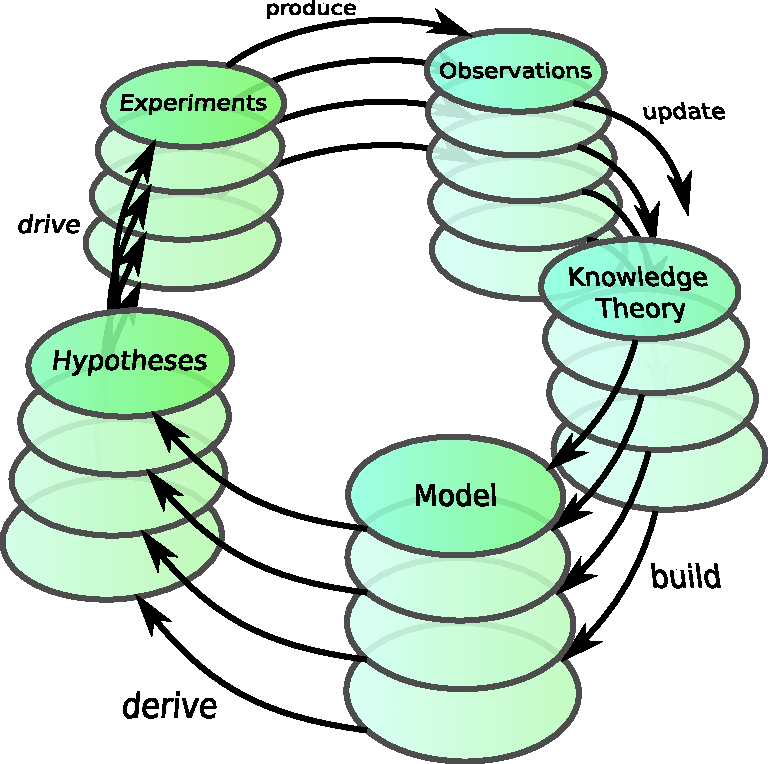
\includegraphics[width=0.35\textwidth]{images/empirical_spiral4}
%  \caption{The empirical spiral: applying the empirical cycle in successive
% rounds leads to a gradual build-up of knowledge.}\label{fig:empirical-spiral}
% \end{figure}


\begin{figure*}[htbp]
\begin{center}
   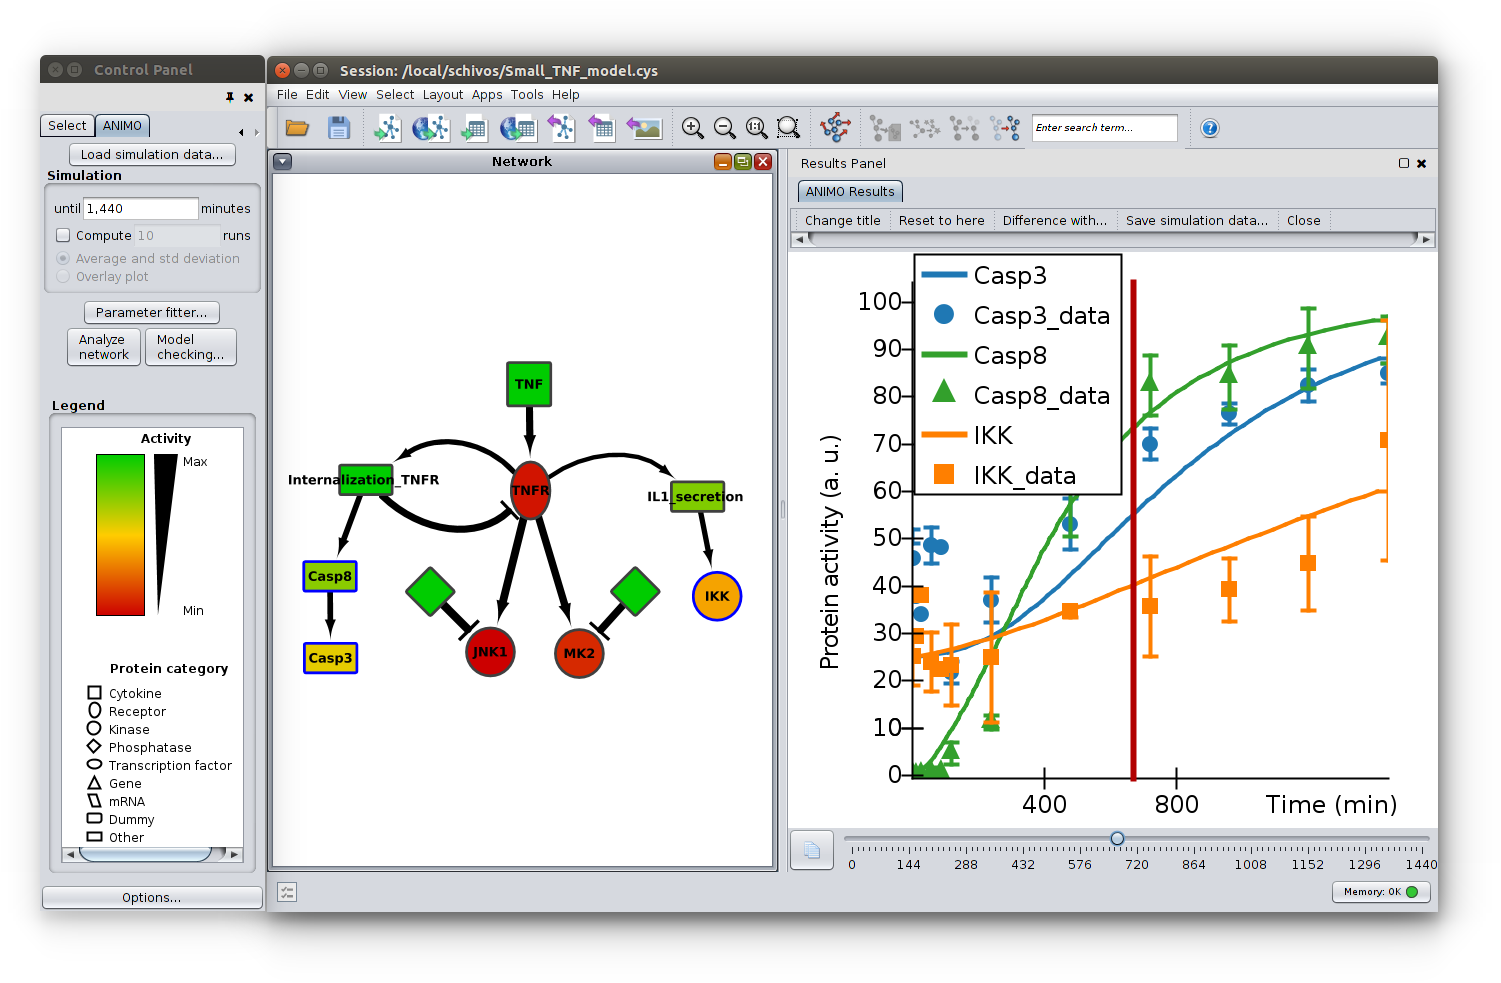
\includegraphics[width=.9\textwidth]{images/screenshotTNFmodelSmall}
\end{center}
\caption{\csentence{The Cytoscape user interface running the ANIMO plug-in.}
The \emph{Network} panel in the center contains the nodes-edges
model of the example TNF$\alpha$ patwhay (see Methods Section~\ref{subsec:case-study}), with
colors indicating node activity levels and shapes representing different protein categories (see the \emph{Legend} on the left).
The \emph{Results Panel} on the right contains a graph plotting activity levels of selected nodes
during the first 24 hours of evolution of the model. The slider under the graph
allows the user to select the time instant (marked as a vertical red line in the graph) on which
the colors nodes in the \emph{Network} are based.
The series with the {\sf \_data} suffix is experimental
data from~\cite{pathway-compendium}, considering a treatment with 100~ng/ml TNF$\alpha$.
\label{fig:cytoscape}}
\end{figure*}


\begin{figure*}[htbp]
 \begin{center}
  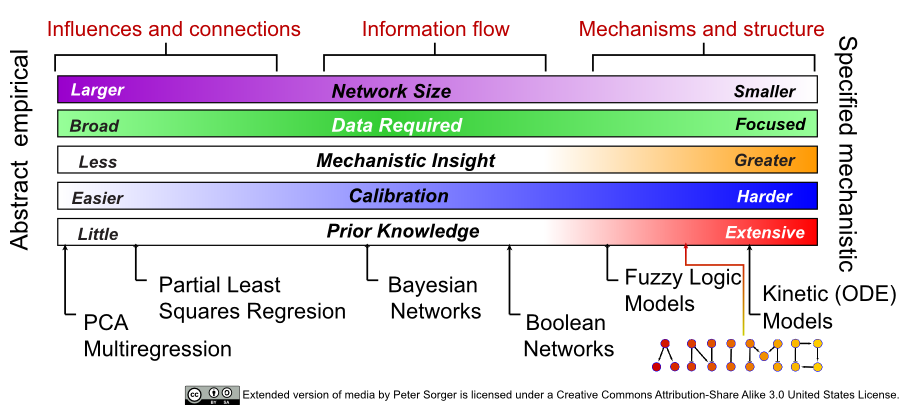
\includegraphics[width=0.9\textwidth]{images/modeling_methods_spectrum_animo}
 \end{center}
\caption{\csentence{The spectrum of modeling methods, with the addition of ANIMO.}
The precision of ANIMO models is halfway between fuzzy logic and ODE. In addition, ANIMO
allows for an easier modeling experience thanks to a user-friendly interface based on
the widely used network modeling software Cytoscape.}
\end{figure*}




\def\drosophilaGraphScale{0.069}%0.123}
\begin{figure*}[!htpb]
\begin{center}
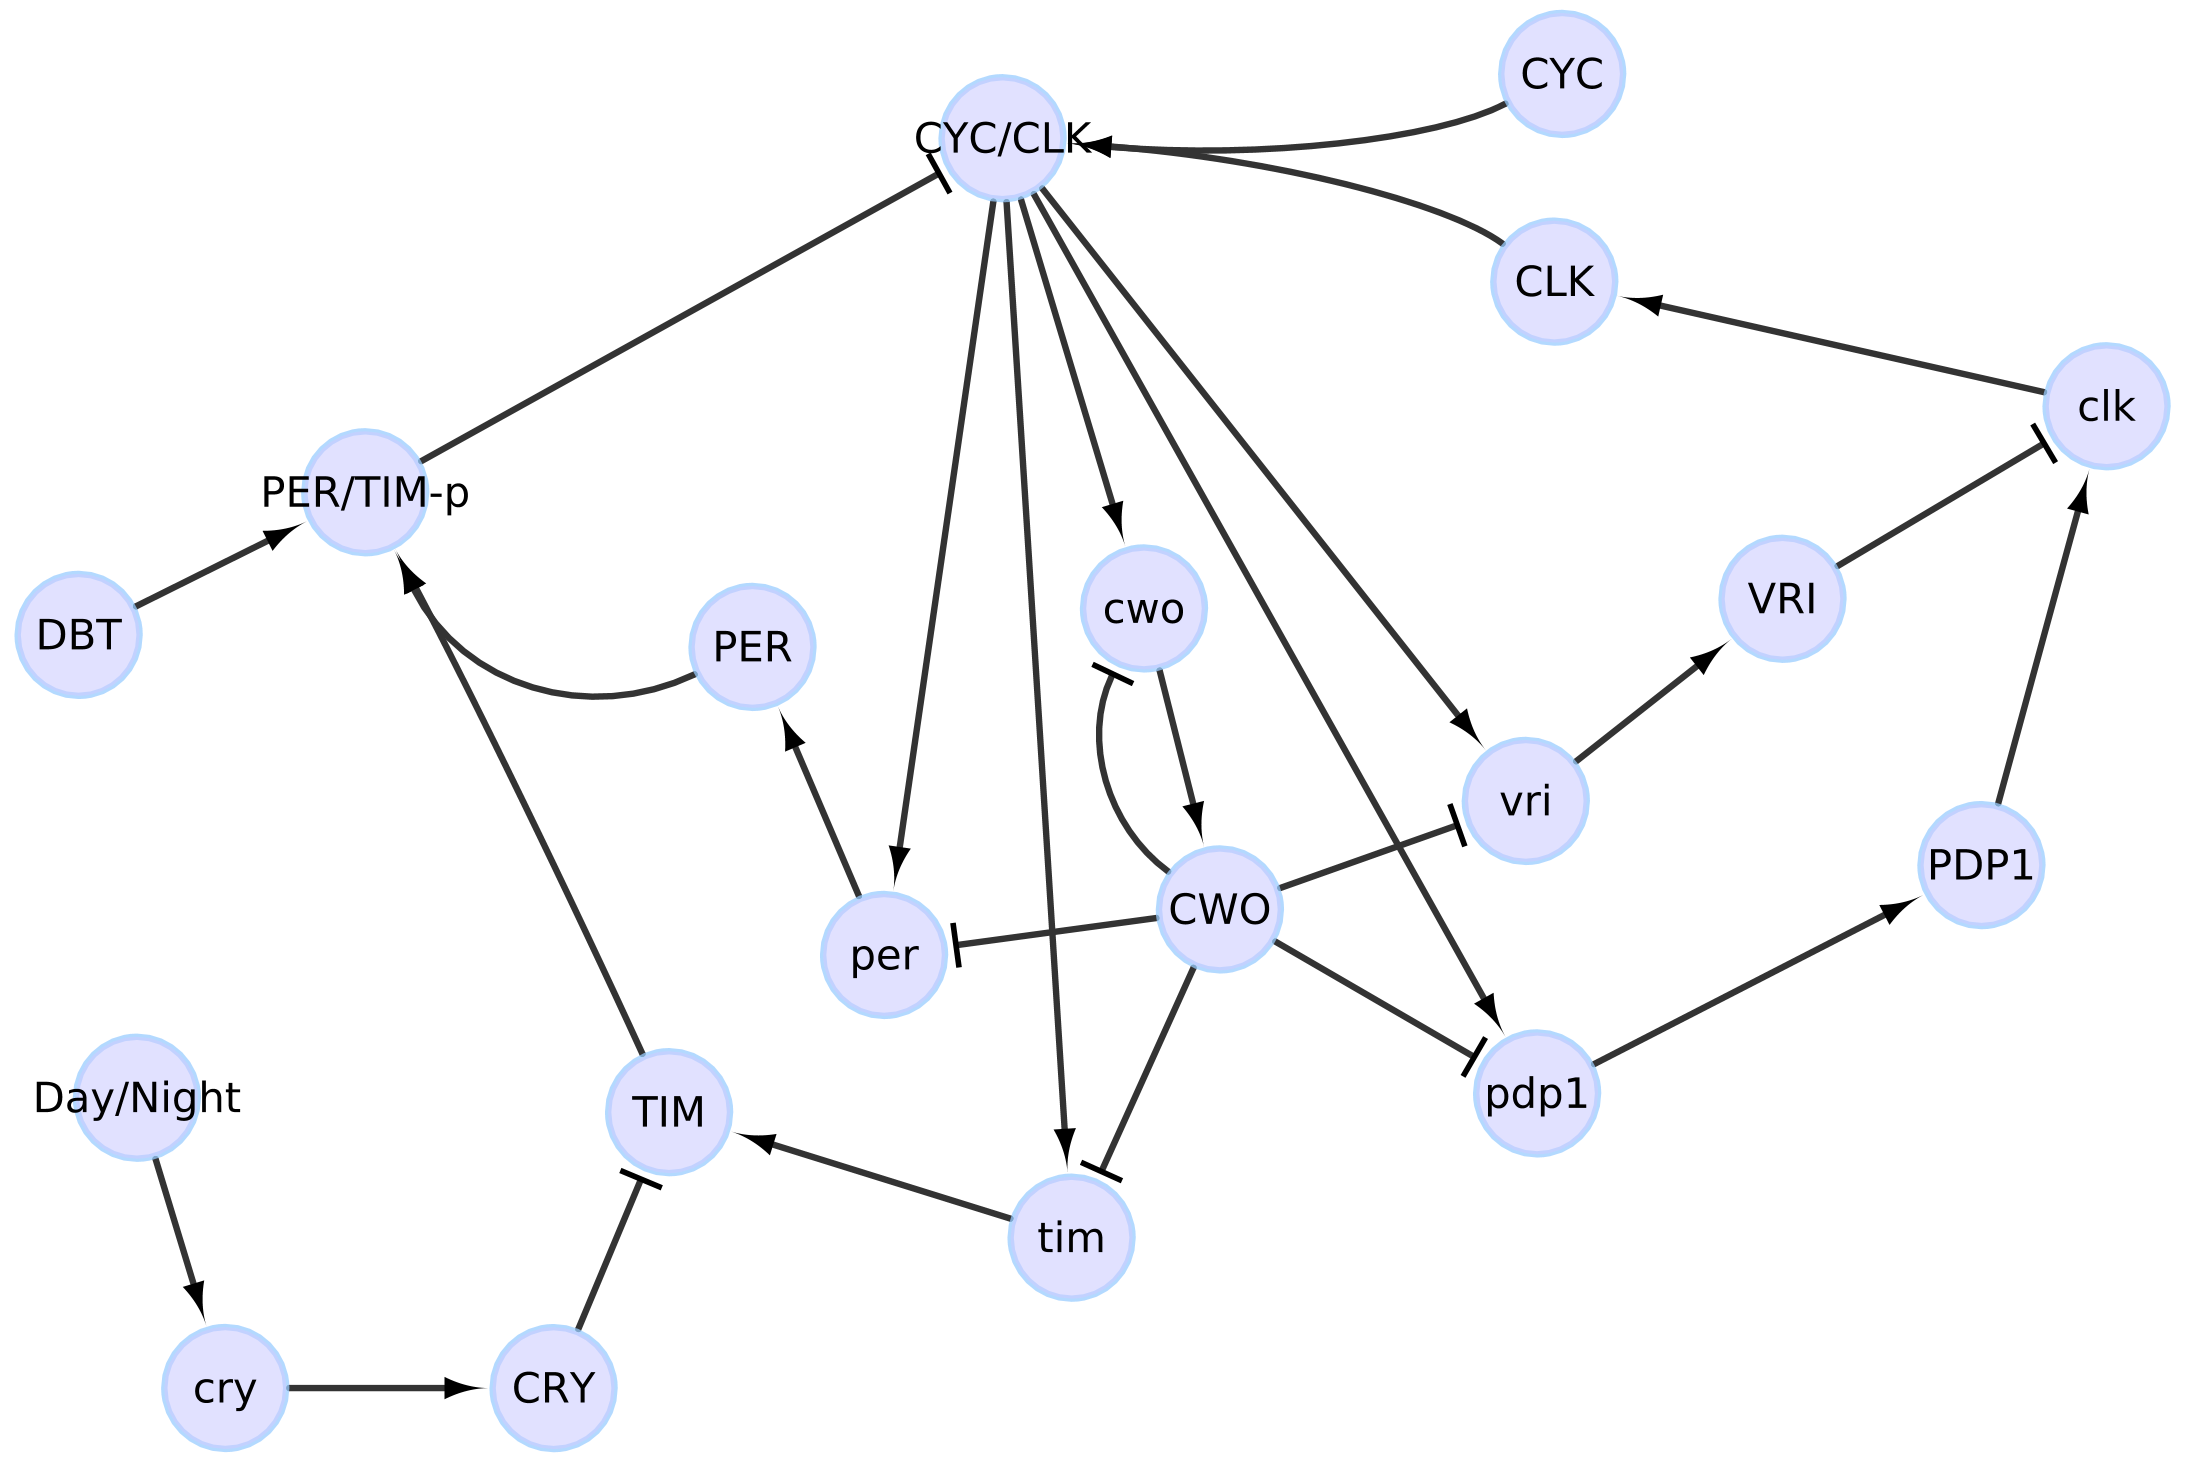
\includegraphics[width=0.49\textwidth]{images/drosophila_model5}%0.85\textwidth
% \subfloat[\label{subfig:drosophila-mrna}]{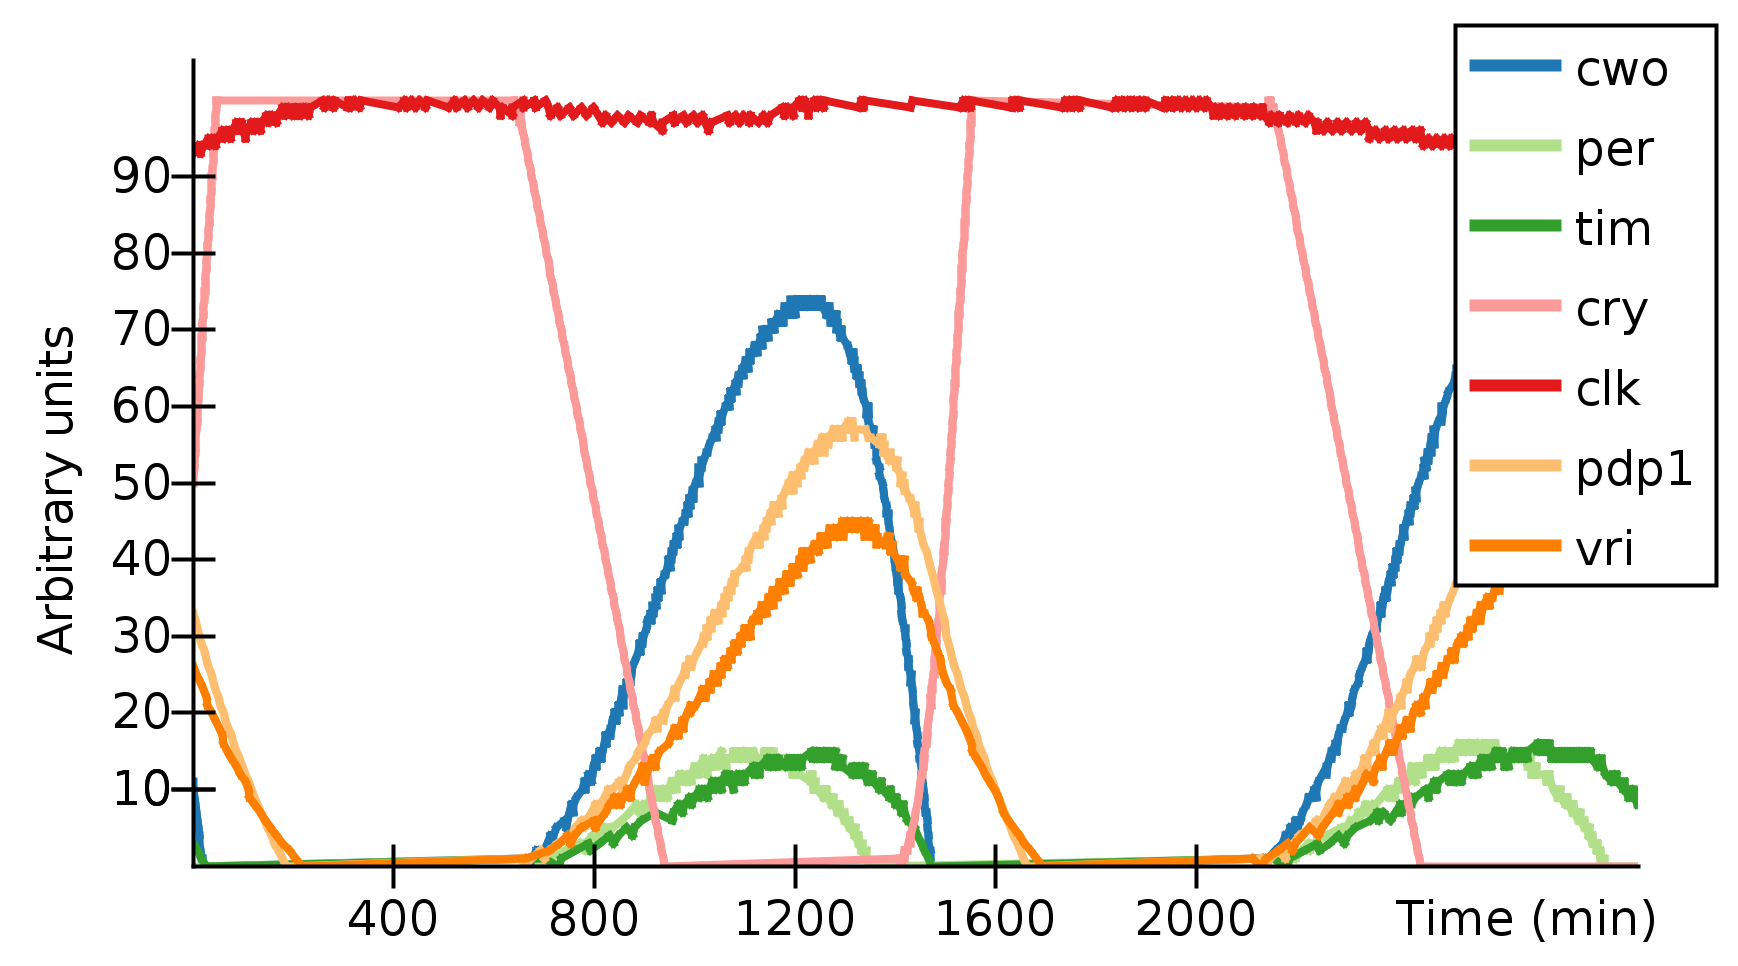
\includegraphics[scale=\drosophilaGraphScale]{images/drosophila_graph2}}\
% \subfloat[\label{subfig:drosophila-proteins}]{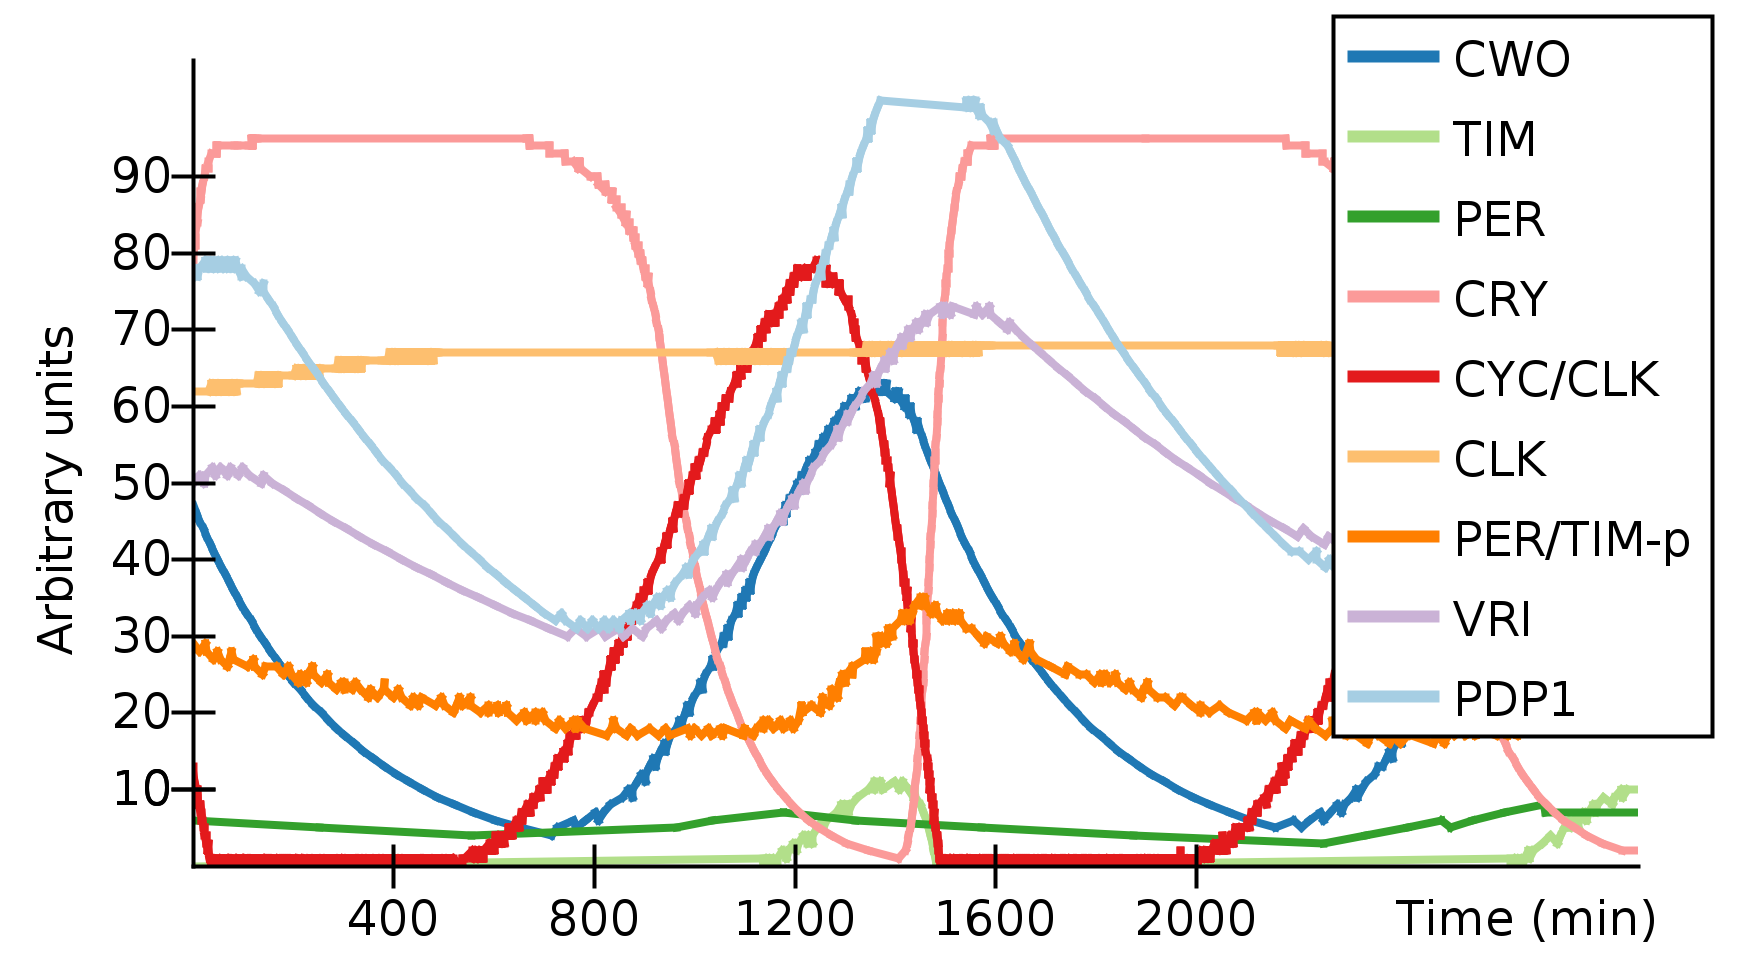
\includegraphics[scale=\drosophilaGraphScale]{images/drosophila_graph1}}
\end{center}
\caption{\csentence{ANIMO model of the circadian clock in \emph{Drosophila Melanogaster}.}
Auto-regulatory negative feedback loops are present on each of the nodes of
the network, following the original model in~\cite{drosophila-ode-model}. These feedback loops ensure that
protein levels decrease over time when activating inputs are absent. The feedback loops are not represented here
for cosmetic reasons only.
% \\ ANIMO plots of the concentration of
% mRNA~{\bfseries \protect\subref{subfig:drosophila-mrna}}
% and proteins~{\bfseries \protect\subref{subfig:drosophila-proteins}} over a period of 48~hours.\\
Naming conventions follow the same rules
as in the original model, with lower-case names representing mRNA, and upper-case names indicating proteins.
}\label{fig:drosophila-model}
\end{figure*}


\def\largeModelScale{0.18}%0.15}%0.155}%0.27}
\def\legendScalaColori{0.21}%0.18}%0.21}
\def\legendScalaForme{0.21}%0.18}%0.21}
\def\scalaGrafici{0.0709}%0.13}
\begin{figure*}[!htpb]
\centering
%  \subfloat[\label{fig:large-model-no-hypotheses}]{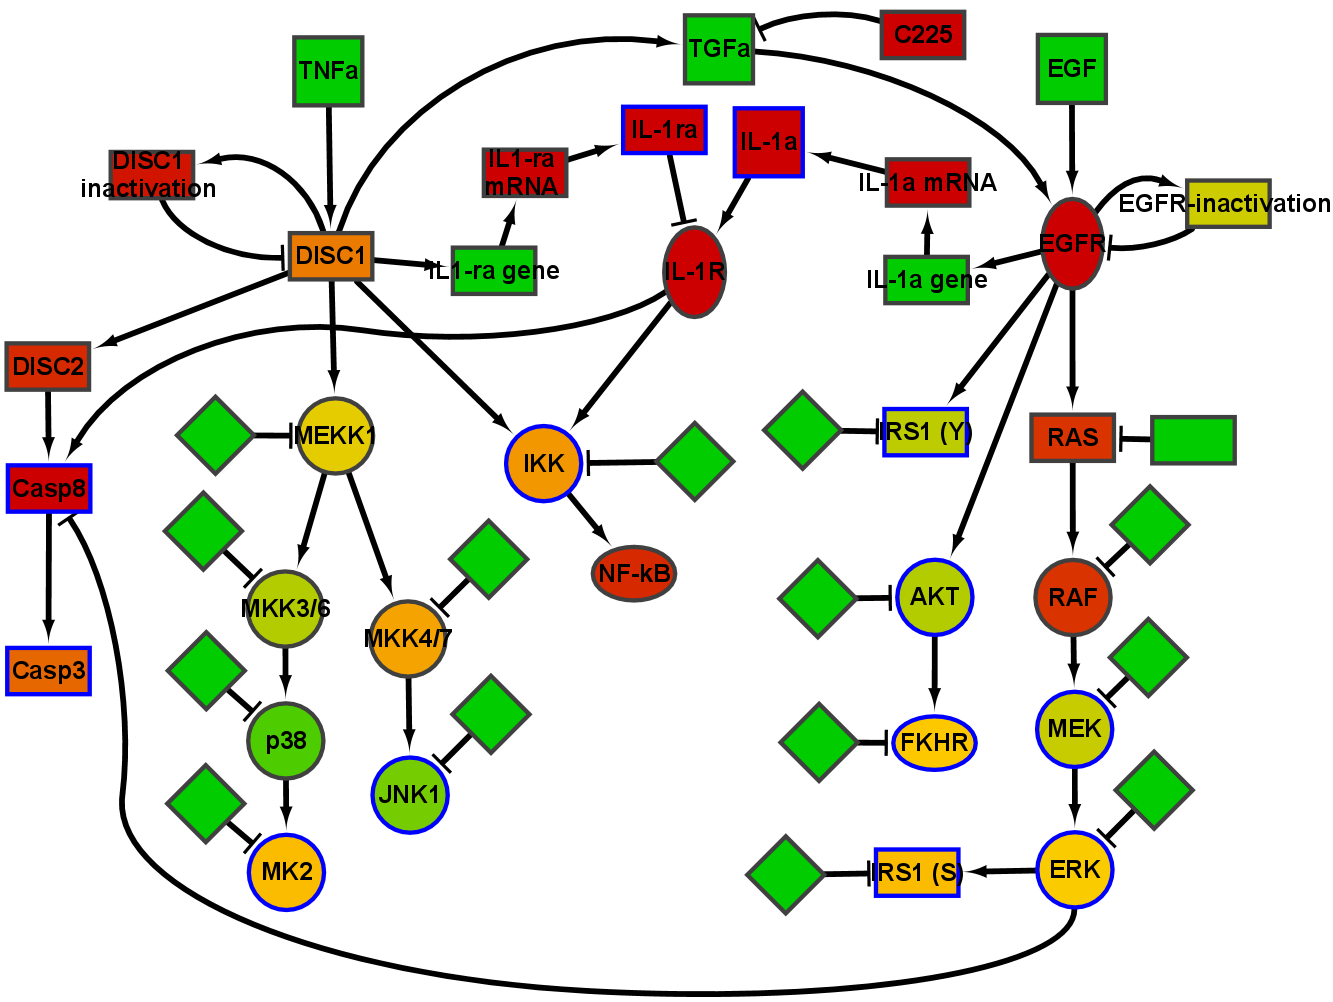
\includegraphics[scale=\largeModelScale]{images/large_network_merged_no_hypotheses}}\\
% %\subfloat{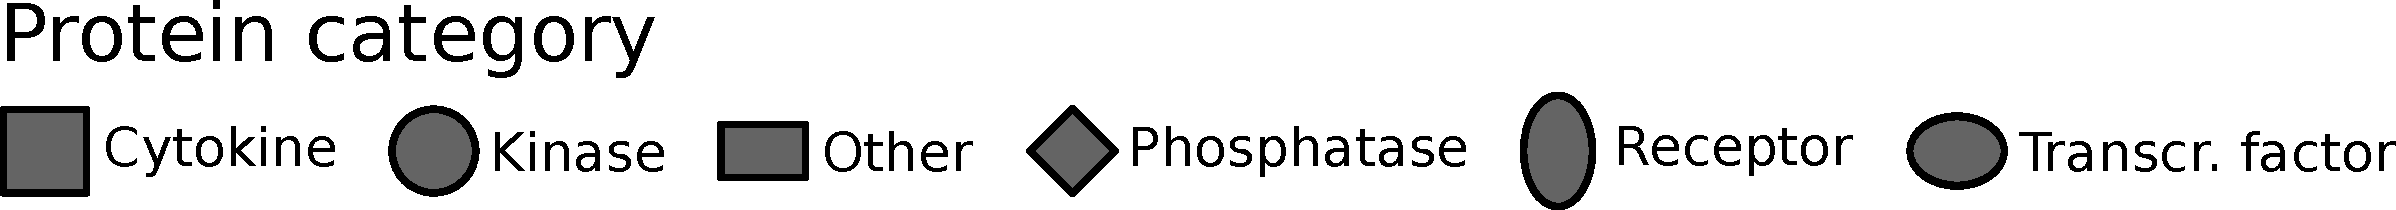
\includegraphics[scale=\legendScalaColori]{images/legenda_forme}}\\ \subfloat{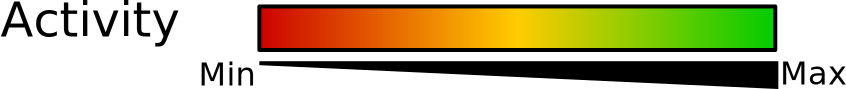
\includegraphics[scale=\legendScalaForme]{images/legenda_colori}}\\
% \subfloat{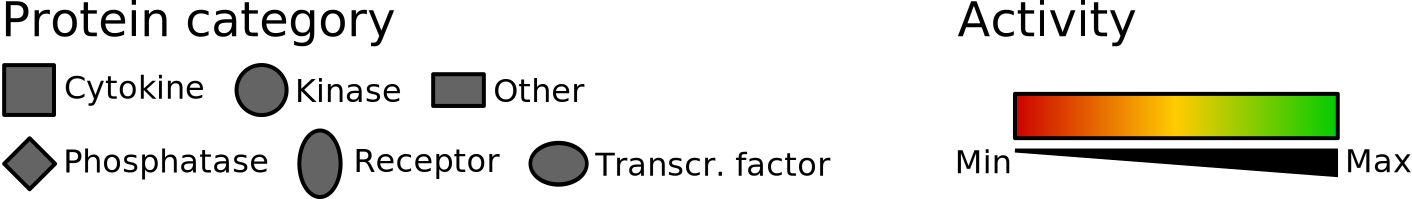
\includegraphics[scale=\legendScalaColori]{images/legenda_forme_e_colori}}\\
% \addtocounter{subfigure}{-1}
% \subfloat[\label{fig:large-model-graph1}]{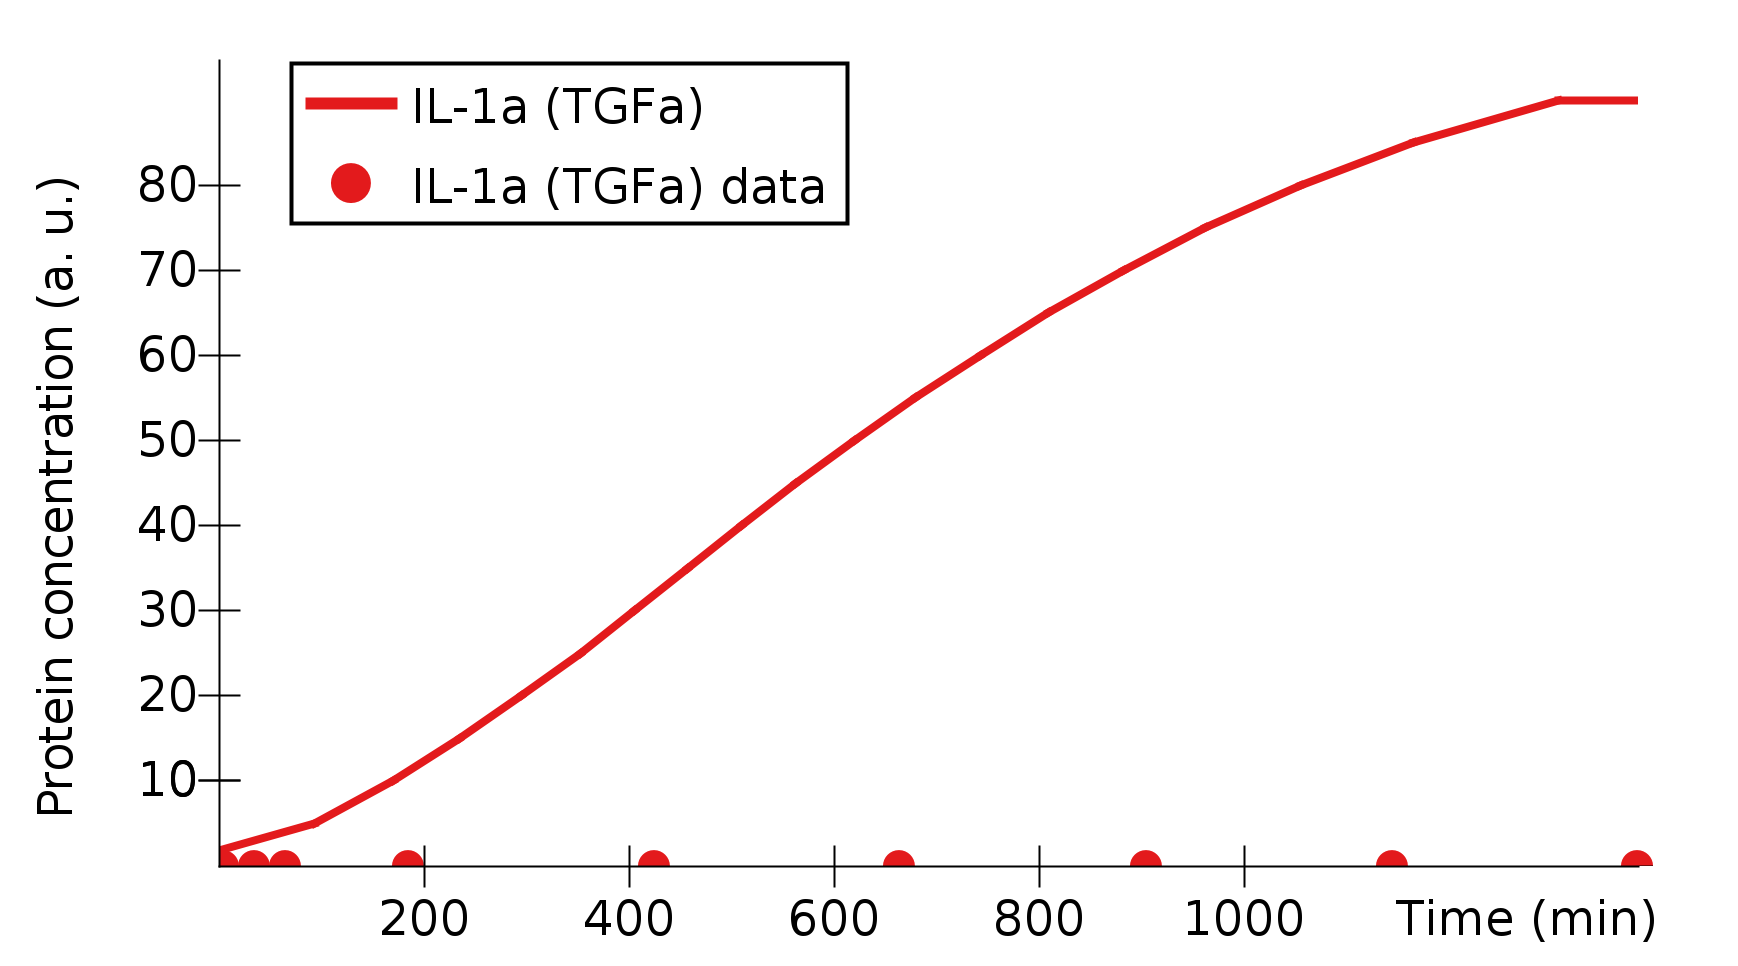
\includegraphics[scale=\scalaGrafici]{images/TGF100_TNF0_ho_hyp_IL-1a3}}
% \subfloat[\label{fig:large-model-graph3}]{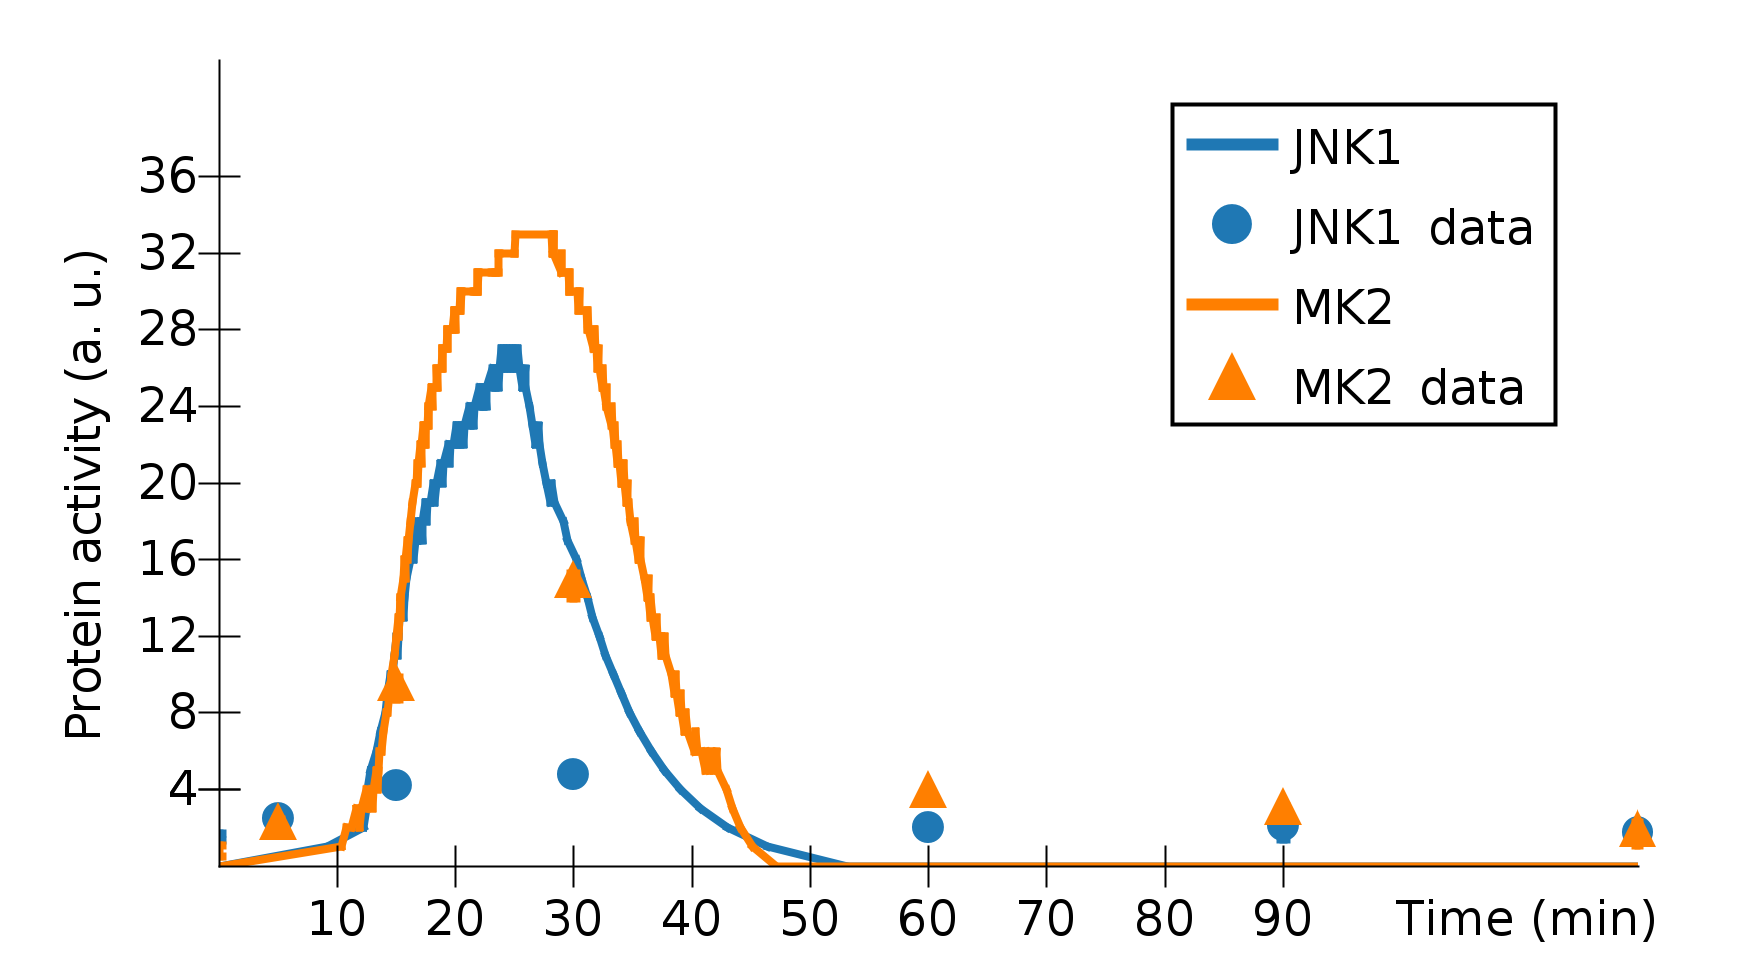
\includegraphics[scale=\scalaGrafici]{images/TNF5_C225_no_hyp_JNK1_MK2}}
  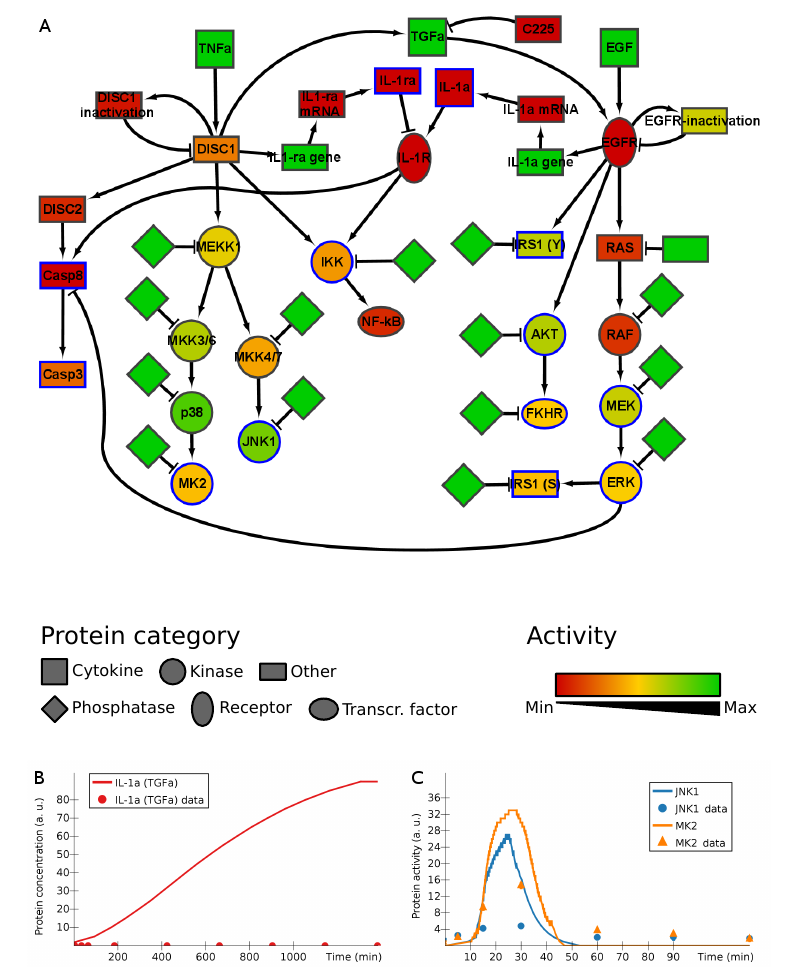
\includegraphics[width=0.9\textwidth]{images/large_network_merged_no_hypotheses_oneImage}
\caption{\csentence{Signaling network downstream of TNF$\alpha$ and EGF in human colon carcinoma cells.}
{\bf(A)} %{\bf \protect\subref{fig:large-model-no-hypotheses}}
The model for the merged TNF$\alpha$ and EGF pathways. Node colors represent the
activity level of the corresponding modeled reactants at time $t = 15$ minutes after
a stimulation of 100 ng/ml TNF$\alpha$ + 100 ng/ml EGF.
{\bf(B)} %{\bf \protect\subref{fig:large-model-graph1}}~
Modeled production of IL-1$\alpha$ after stimulation with 100 ng/ml TGF$\alpha$ (24 hours).
{\bf(C)} %{\bf \protect\subref{fig:large-model-graph3}}~
Modeled activation of JNK1 and MK2 after stimulation with 5 ng/ml TNF$\alpha$ + 10 $\mu$g/ml C225 (2 hours).
\\
The {\sf \_{}data} suffix identifies experimental data; all other series are computed by ANIMO.}\label{fig:large-model-all}
\end{figure*}


\begin{figure*}[!tpb]
\begin{center}
% \subfloat[\label{fig:large-model-complete}]{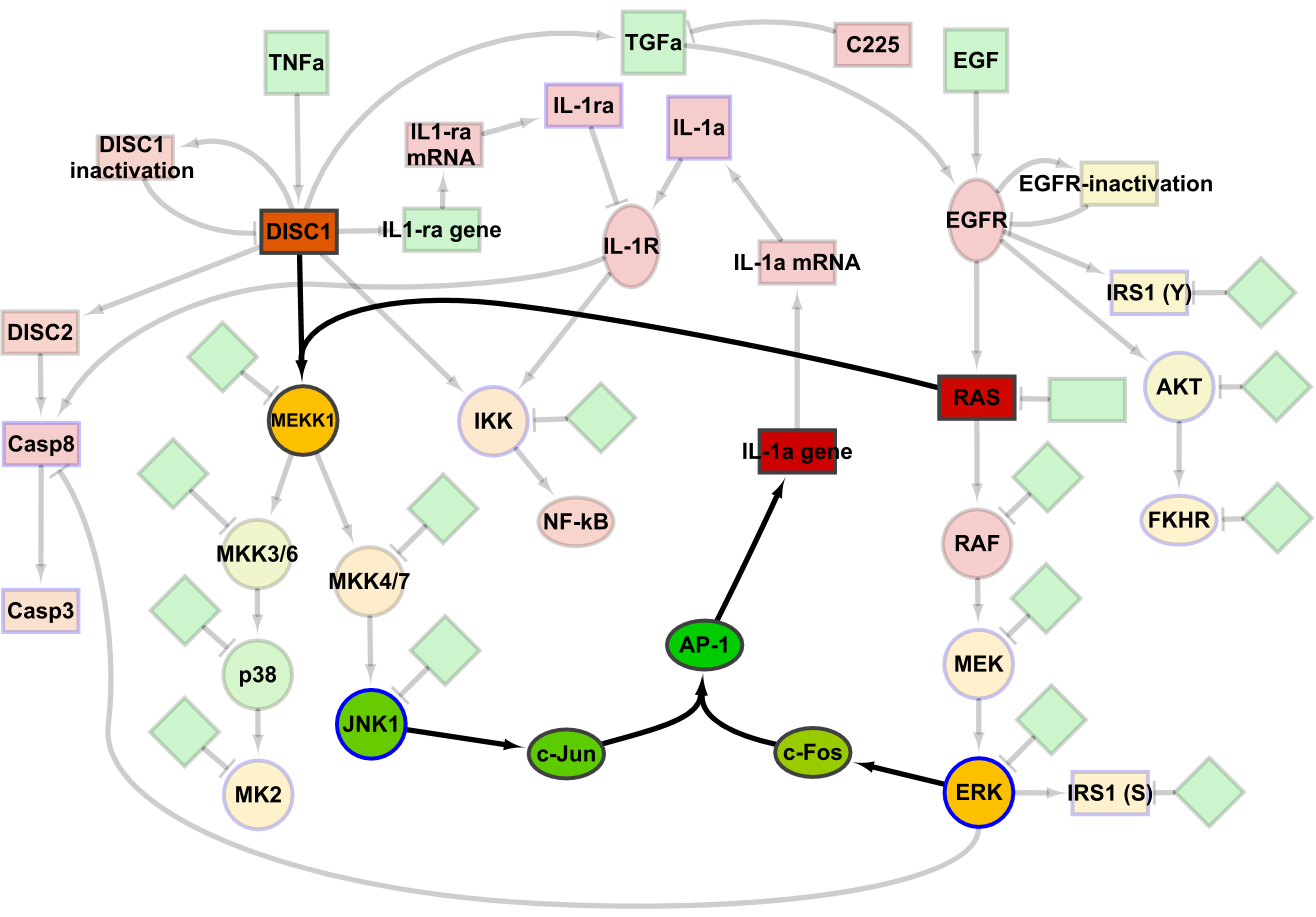
\includegraphics[scale=\largeModelScale]{images/large_network_legendg}}\\
%  \subfloat[\label{fig:large-model-graph2}]{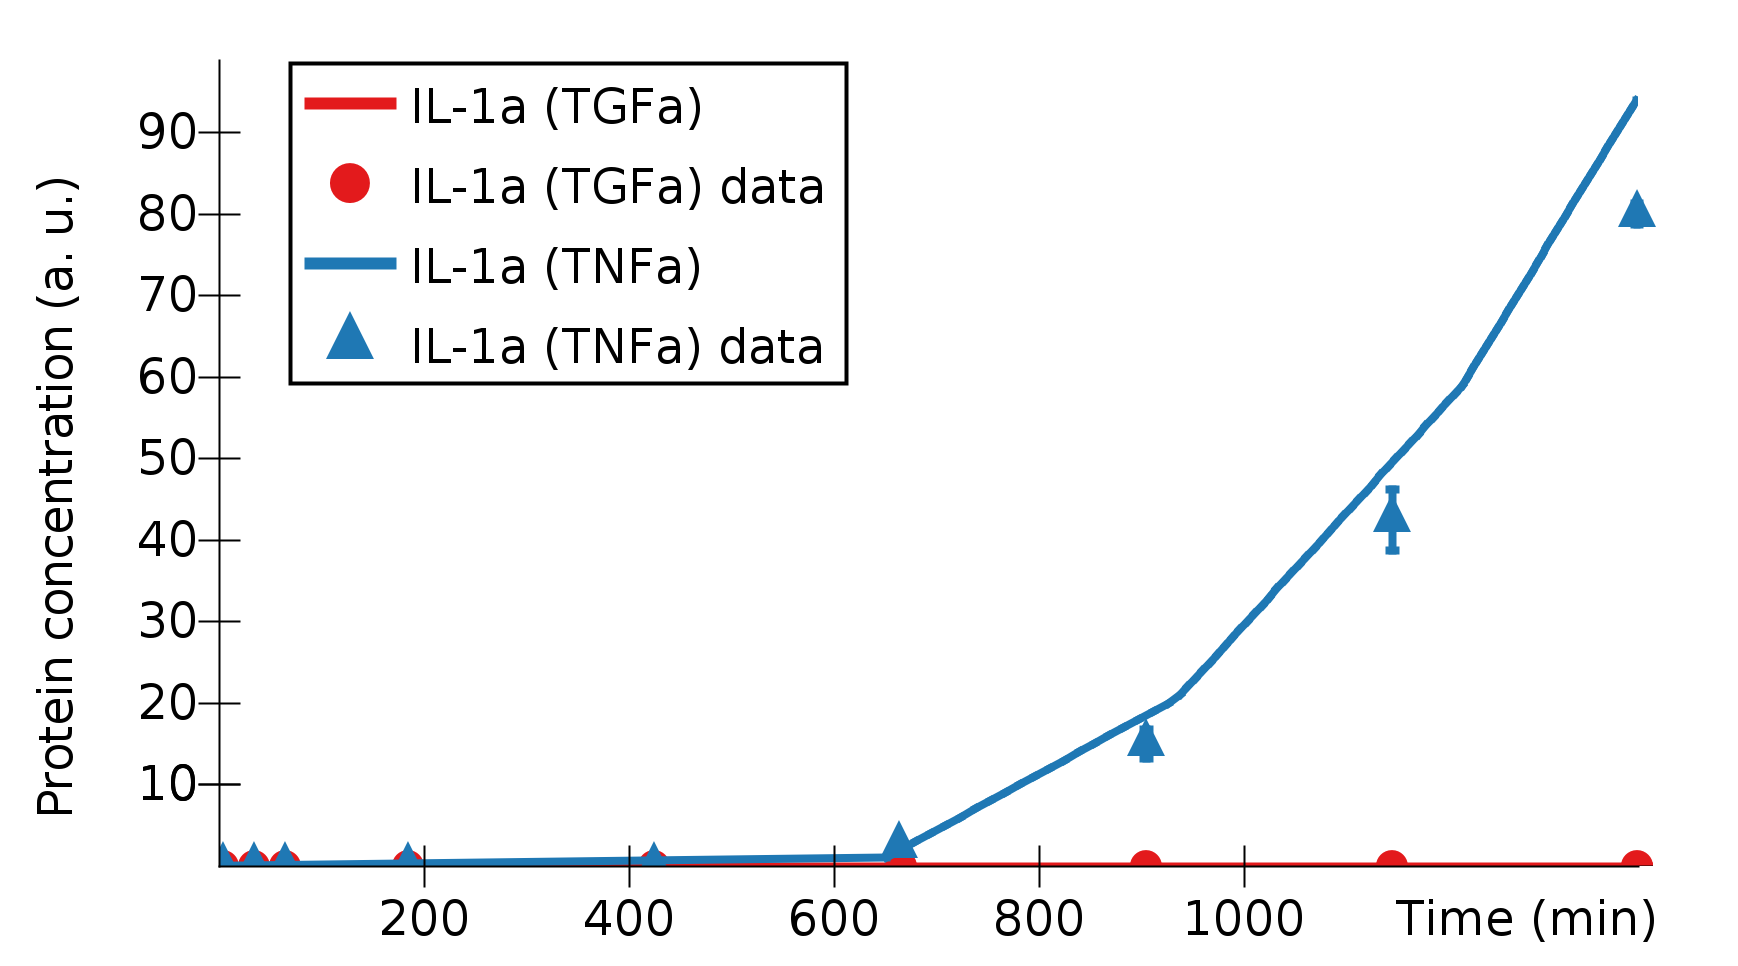
\includegraphics[scale=\scalaGrafici]{images/TGF100_vs_TNF100_hyp1_IL-1a4}}
%  \subfloat[\label{fig:large-model-graph4}]{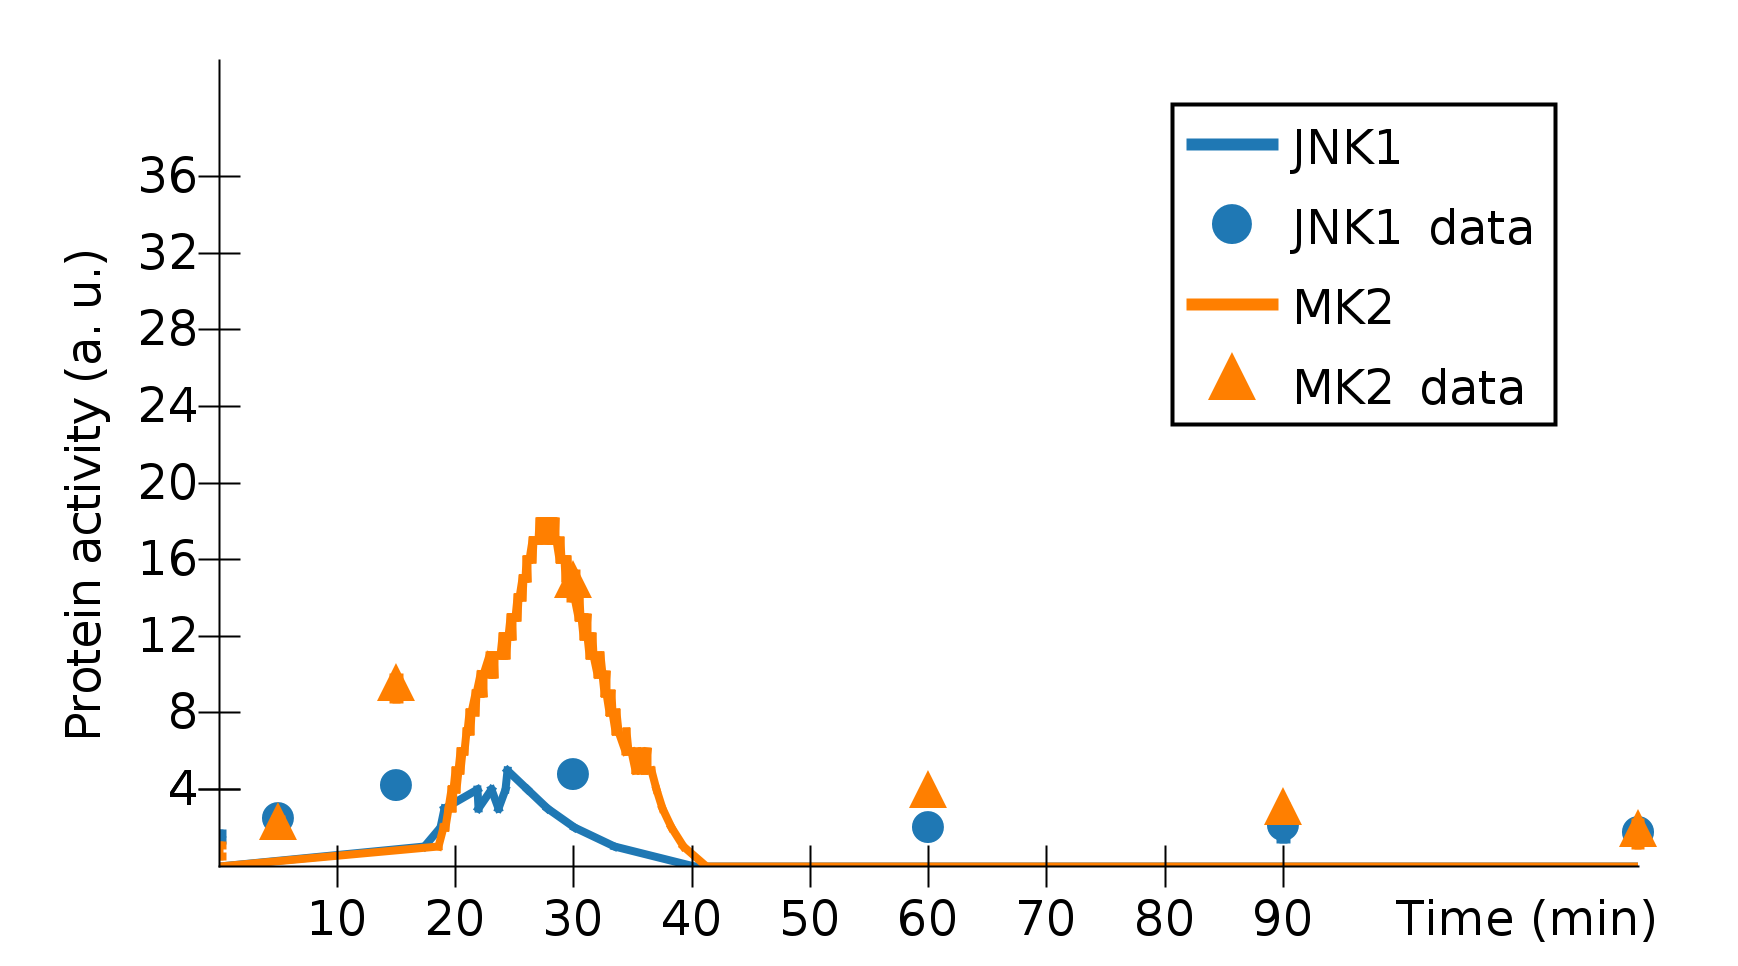
\includegraphics[scale=\scalaGrafici]{images/TNF5_C225_hyp2_JNK1_MK2}}
  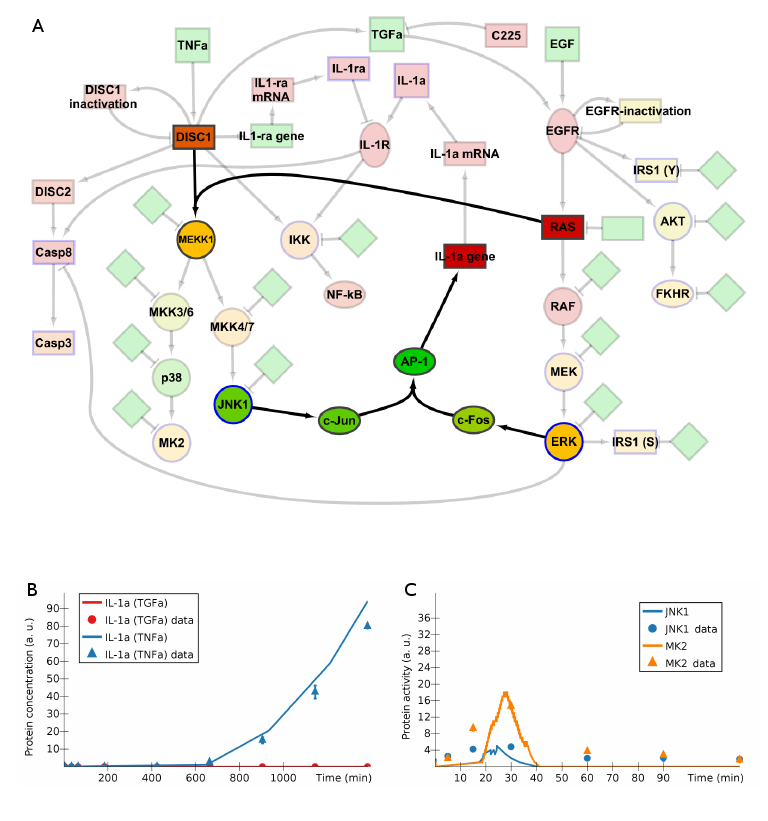
\includegraphics[width=0.9\textwidth]{images/large_network_legendg_oneImage}
\end{center}
\caption{\csentence{Signaling network downstream of TNF$\alpha$ and EGF in human colon carcinoma cells: updated version.}
{\bf(A)} %{\bf \protect\subref{fig:large-model-complete}}
The model for the merged TNF$\alpha$ and EGF pathways
after addition of the two hypotheses (highlighted).
Hypothesis 1 assumes IL-1$\alpha$ expression to depend on AP-1 activity, which in turn requires
both c-Jun en c-Fos to be activated by JNK1 and ERK, respectively. Hypothesis 2 assumes RAS as an activator
of MEKK1. Node colors represent the activity levels $15$ minutes
after stimulation of 100 ng/ml TNF$\alpha$ + 100 ng/ml EGF.
{\bf(B)} %{\bf \protect\subref{fig:large-model-graph2}}~
After the addition of the first hypothesis (activation of IL-1$\alpha$ production depending both
on JNK1 and ERK): production of IL-1$\alpha$ after stimulation with 100 ng/ml TNF$\alpha$ (series {\sf IL-1a~(TNFa)})
compared with stimulation with 100 ng/ml TGF$\alpha$ (series {\sf IL-1a~(TGFa)}) (24 hours).
{\bf(C)} %{\bf \protect\subref{fig:large-model-graph4}}~
After the addition of the second hypothesis (activation of MEKK1 downstream of EGFR):
stimulation with 5 ng/ml TNF$\alpha$ + 10 $\mu$g/ml C225 (2 hours).
Suppl. Sect.~\ref{suppl:parameters-tnf-egf} explains how the dosage of 5 ng/ml TNF$\alpha$ was represented in the model.\\
The {\sf \_{}data} suffix identifies experimental data; all other series are computed by ANIMO.}\label{fig:large-model-graph}\label{fig:large-model-complete}
\end{figure*}





\def\modelGraphScale{0.148}%0.215}
\def\legendGraphScale{0.16}
\def\halfGraphScale{0.067}%0.1075}
\begin{figure*}[!h]
%\begin{floatingfigure}[l]{.45\textwidth}
\begin{center}
% \subfloat[\label{subfig:mek-erk}]{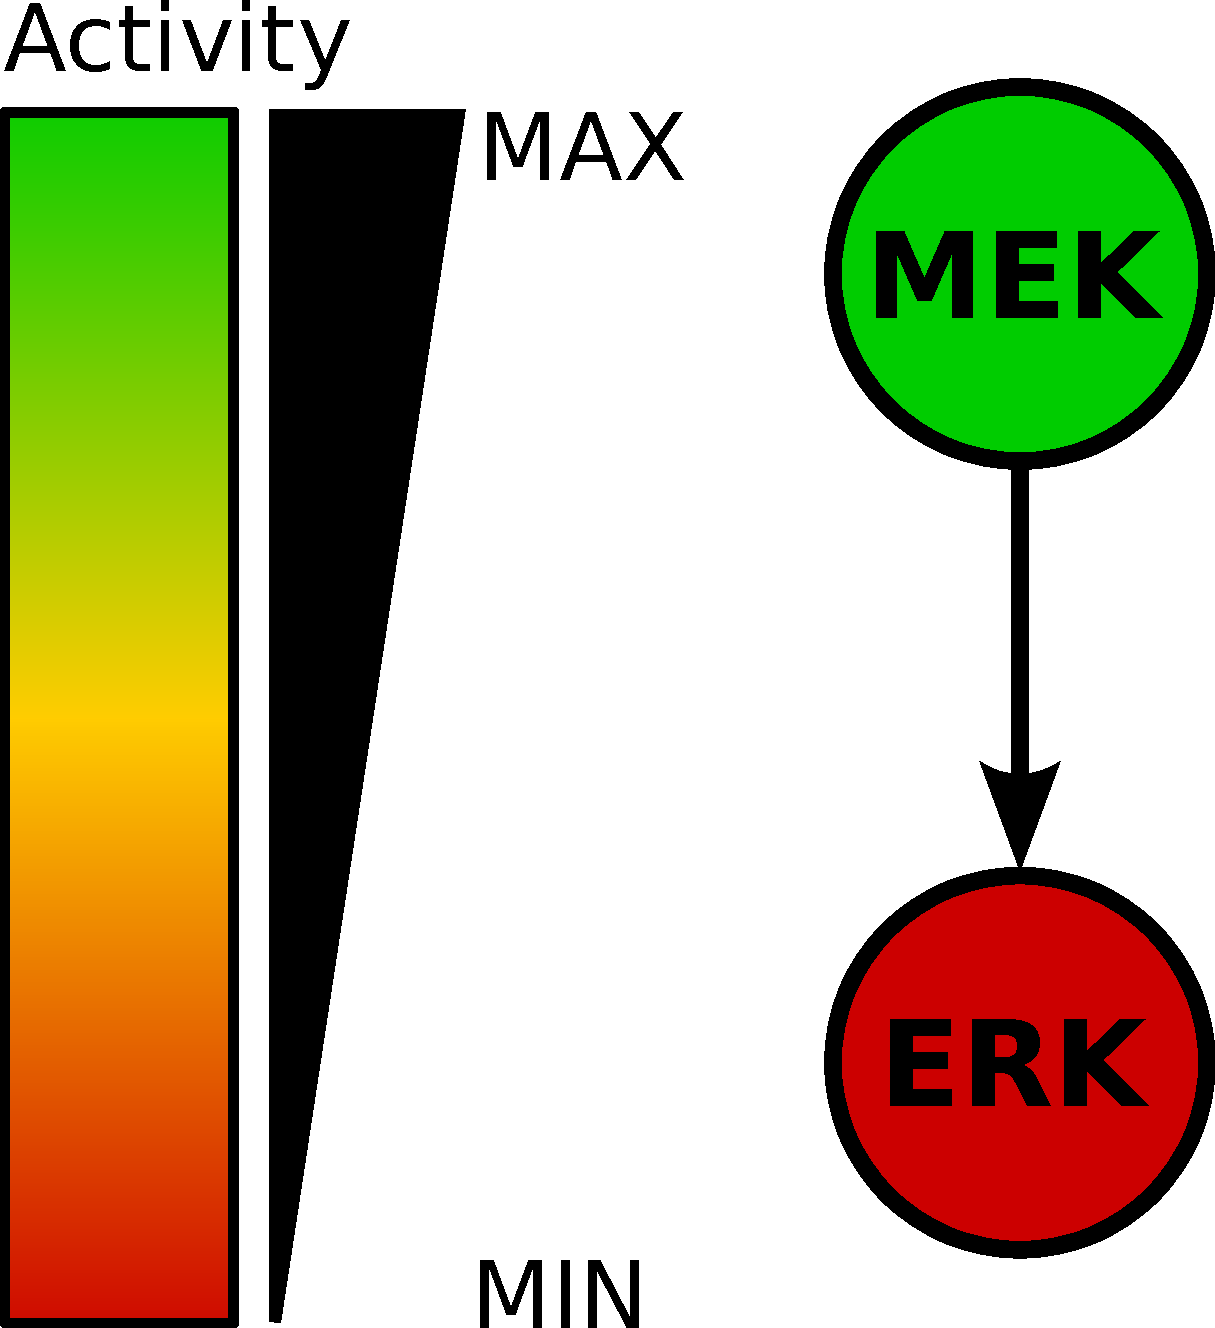
\includegraphics[scale=.098]{images/abstraction_ta_mek-erk3}}
%   \quad%\qquad\qquad
% \subfloat[\label{subfig:erk}]{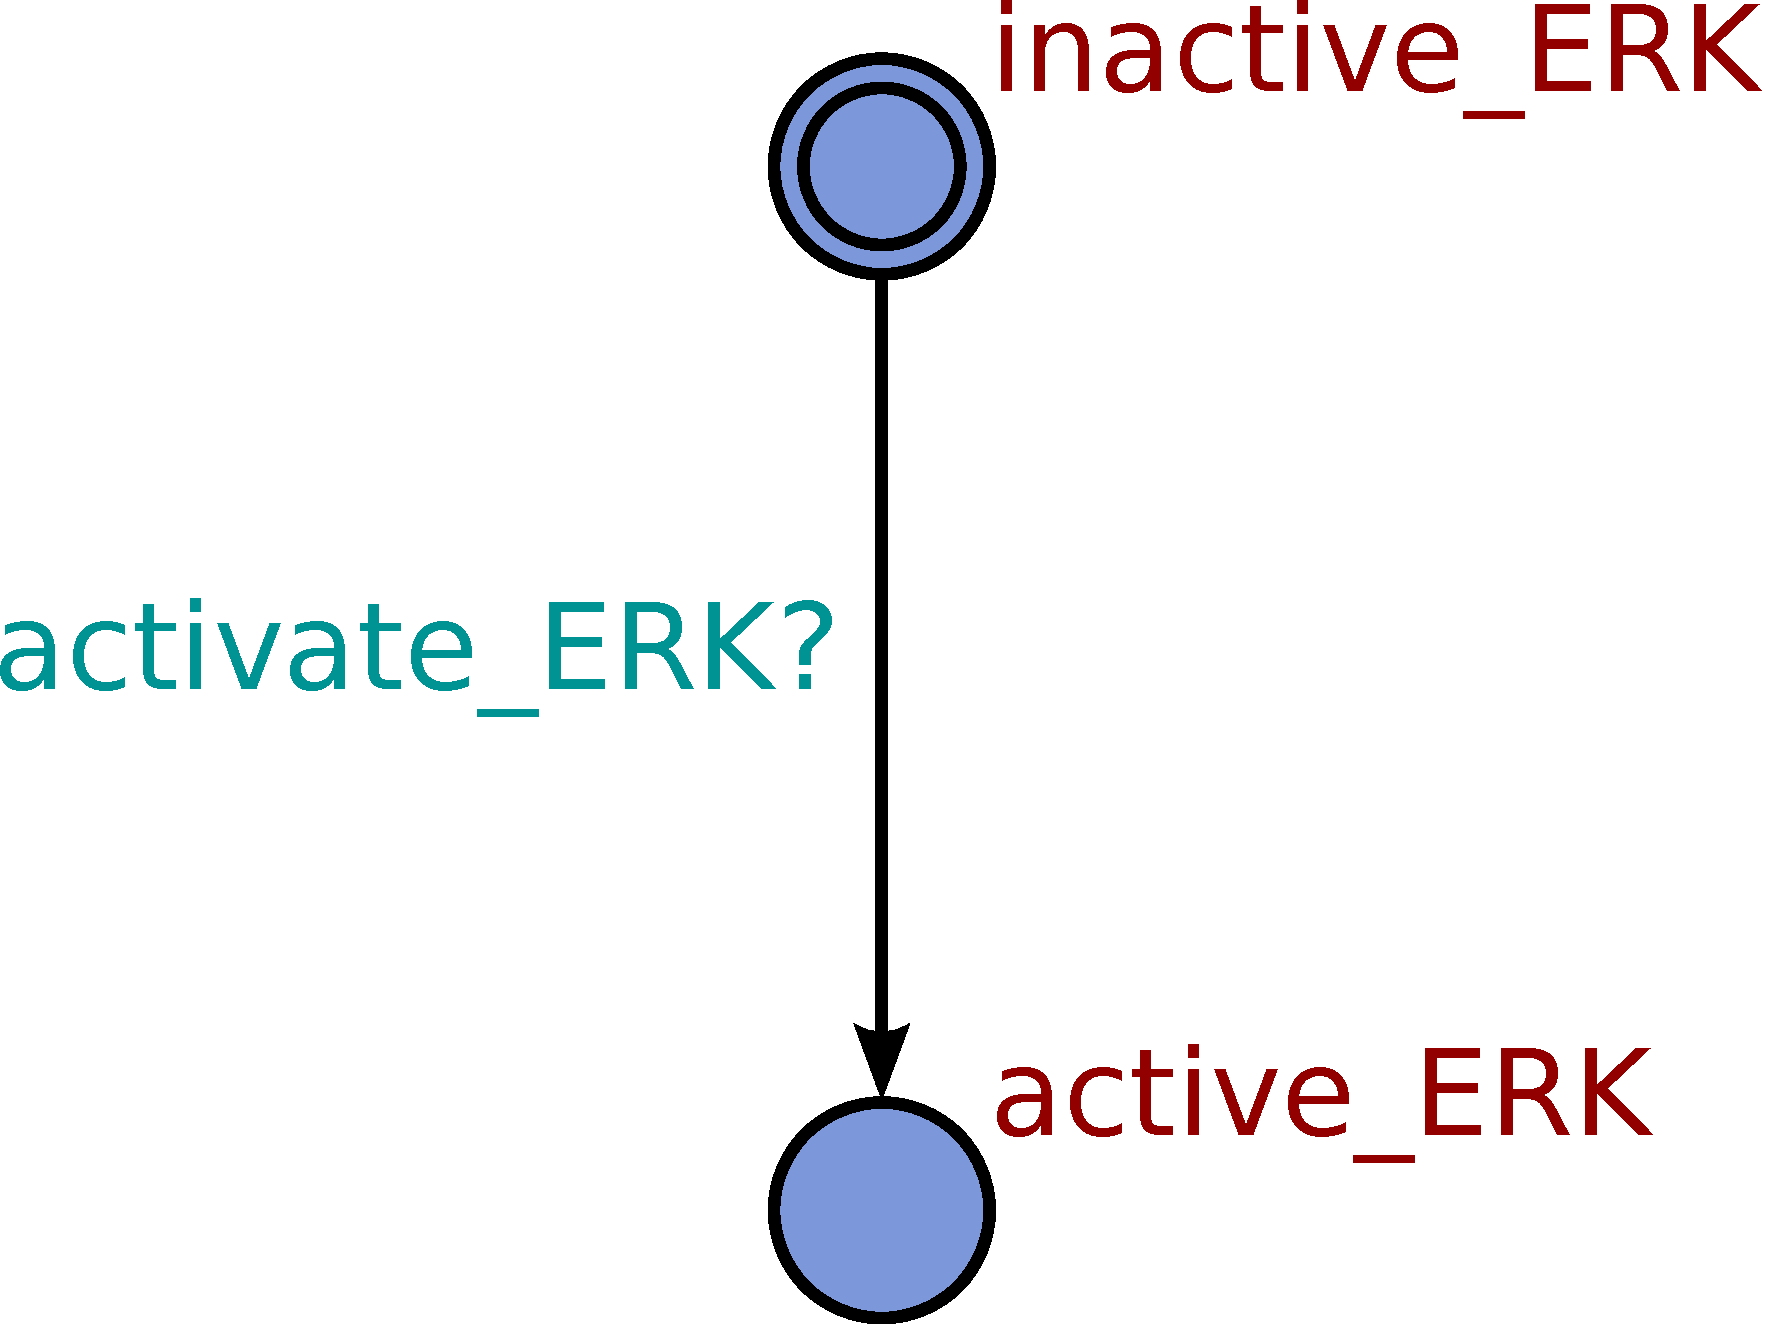
\includegraphics[scale=.098]{images/abstraction_ta_erk}}
%   \quad%\qquad\qquad
% \subfloat[\label{subfig:mek}]{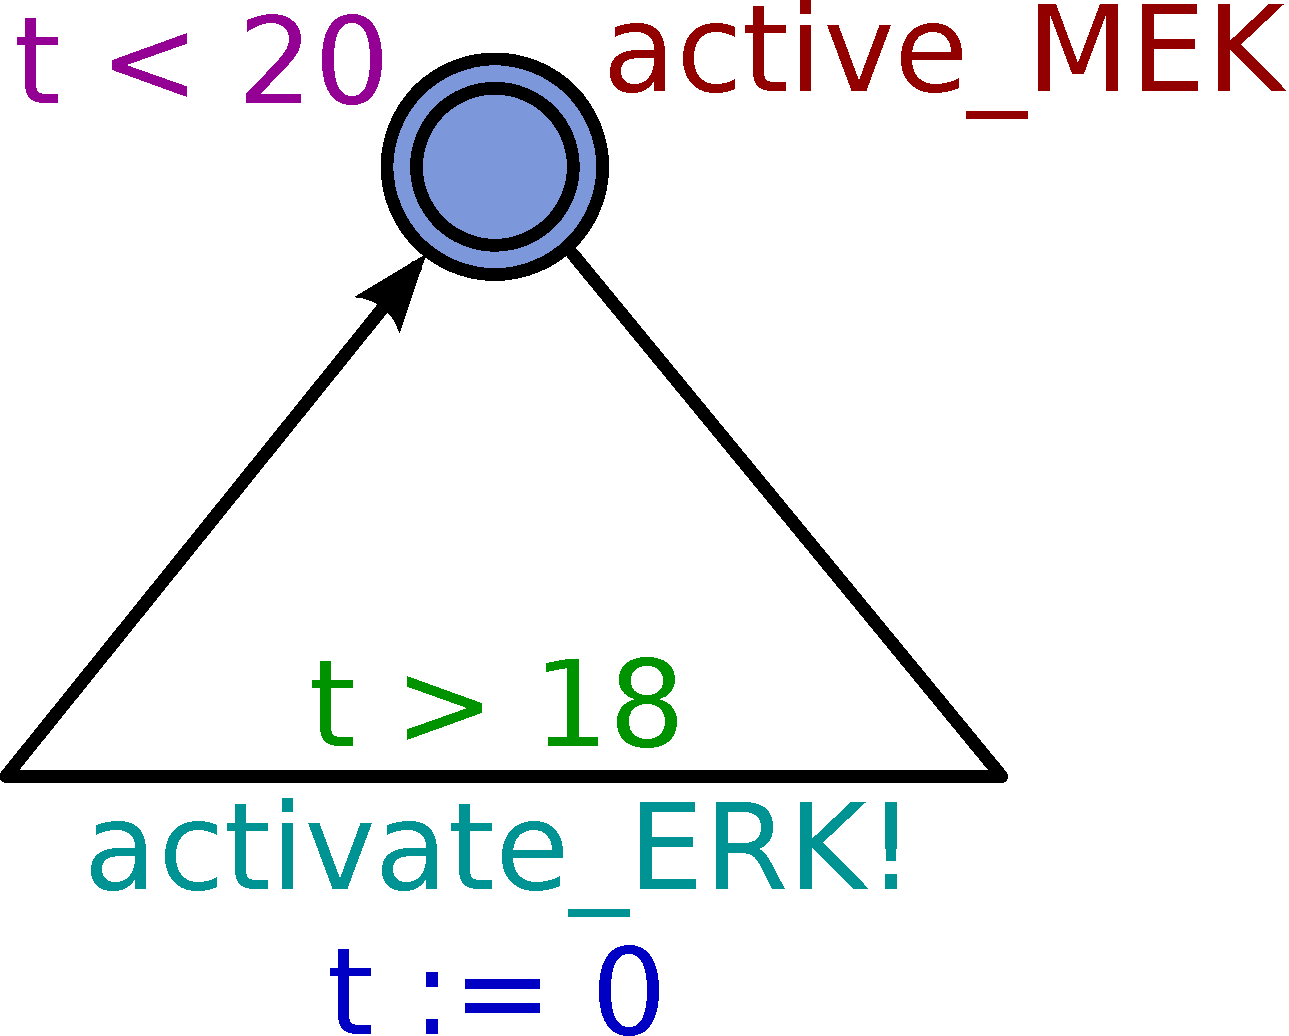
\includegraphics[scale=.098]{images/abstraction_ta_mek}}
  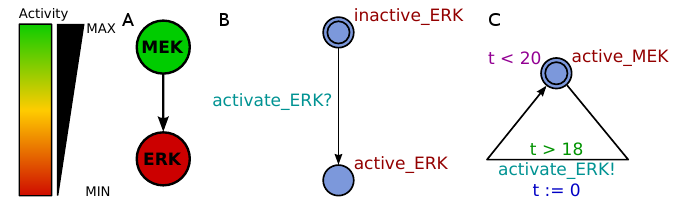
\includegraphics[width=0.7\textwidth]{images/abstraction_ta_mek-erk3_oneImage}
\end{center}
\caption{\csentence{Abstraction of a biochemical reaction to a \tas\ model.}
{\bf(A)} %{\bf \protect\subref{subfig:mek-erk}}~
Classical depiction of a well-studied intracellular signal transduction reaction: protein
MAPK-ERK kinase (MEK) activates downstream protein extracellular-regulated kinase (ERK).
{\bf(B)} %{\bf \protect\subref{subfig:erk}}~
A \ta\ model of ERK, consisting of two states (circles), {\sf inactive\_ERK} and {\sf active\_ERK},
and one transition (arrow) between the states. This transition will take place when it is possible to synchronize with
the corresponding action {\sf activate\_ERK!} in the MEK automaton.
{\bf(C)} %{\bf \protect\subref{subfig:mek}}~
A \ta\ model of active MEK, consisting of one state and one
transition. ${\sf t} < 20$ is termed an invariant on the state, allowing residence in this state as long as local
clock time {\sf t} is smaller than $20$ units. ${\sf t} > 18$ is termed a guard on the transition, allowing the
transition to take place when local clock {\sf t} is greater than $18$ units. Together, the invariant and guard in this
example ensure that the transition must take place in the (continuous) time interval $18 < {\sf t} < 20$. When the
transition takes place, the action {\sf activate\_Erk!} is performed (thus allowing the ERK automaton to reach the {\sf
active\_ERK} state) and the local clock coupled to this automaton is reset, ${\sf t} := 0$.\label{fig:abstraction-mek-erk}}
\end{figure*}


\begin{figure*}[h!]
\centering
%  \\
% \subfloat{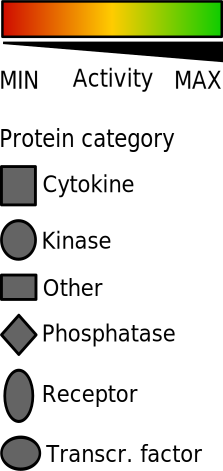
\includegraphics[scale=\legendGraphScale]{images/small-model-1g_legenda}}\addtocounter{subfigure}{-1}\subfloat[\label{fig:small-model-first}]{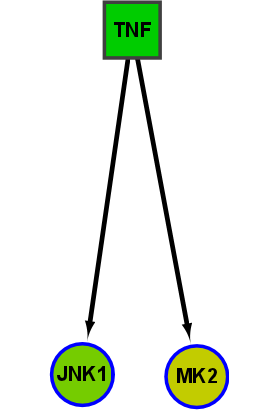
\includegraphics[scale=\modelGraphScale]{images/00-paper-model1f}}
% %\subfloat[\label{fig:small-model-second}]{\includegraphics[scale=\modelGraphScale]{images/00-paper-model2f}}
% \subfloat[\label{fig:small-model-third}]{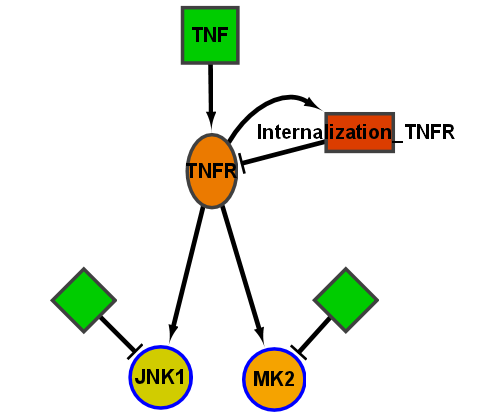
\includegraphics[scale=\modelGraphScale]{images/00-paper-model3f}}
% \subfloat[\label{fig:small-model-fourth}]{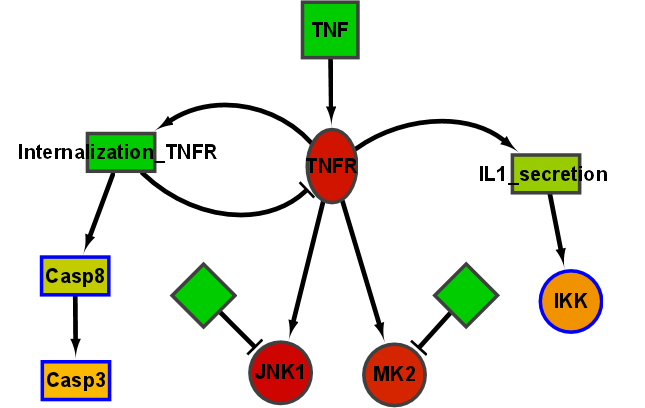
\includegraphics[scale=\modelGraphScale]{images/00-paper-model4g}}
%    \\
% \subfloat[\label{fig:small-model-first-graph}]{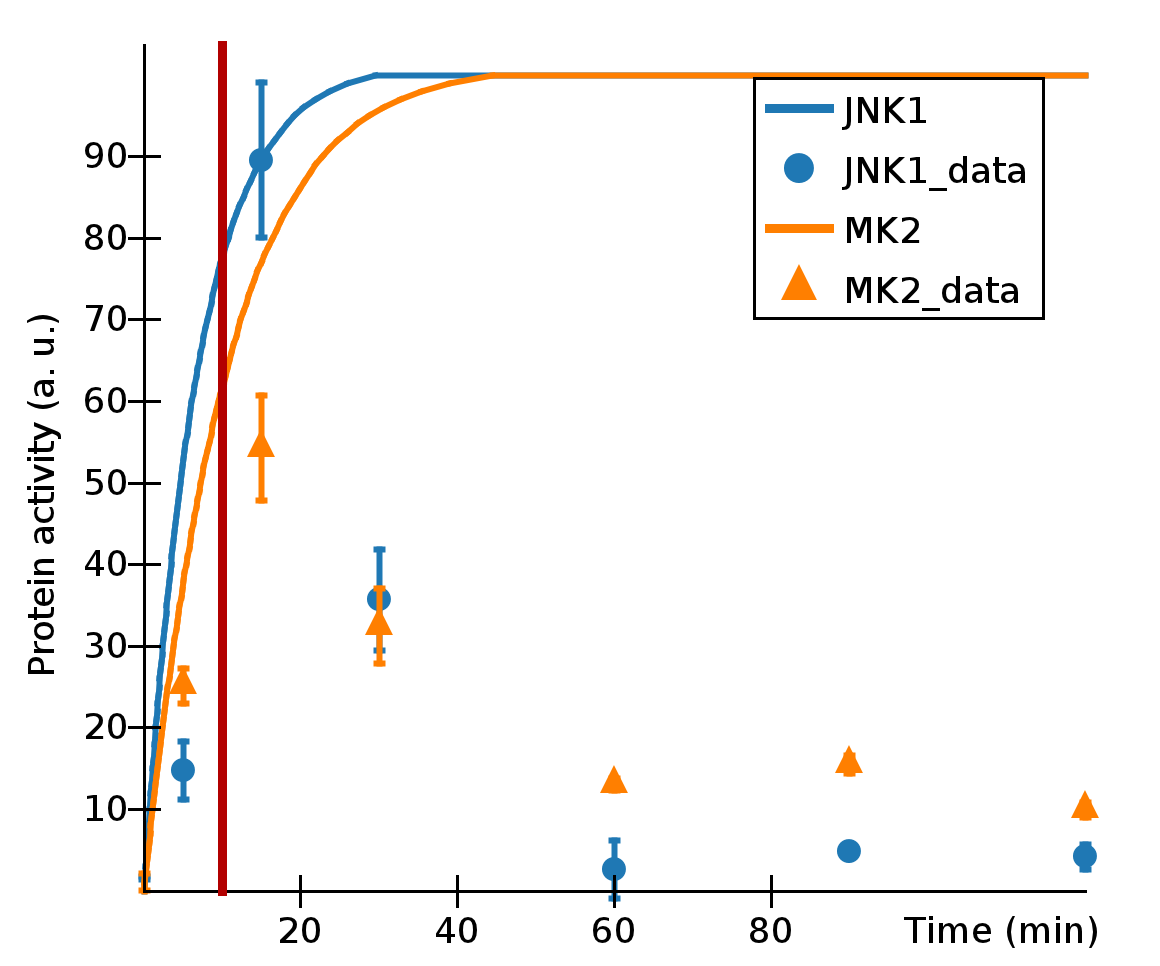
\includegraphics[scale=\halfGraphScale]{images/00-paper-graph1m_riga}}
% %\subfloat[\label{fig:small-model-second-graph}]{\includegraphics[scale=\halfGraphScale]{images/00-paper-graph2m_riga}}
% \subfloat[\label{fig:small-model-third-graph}]{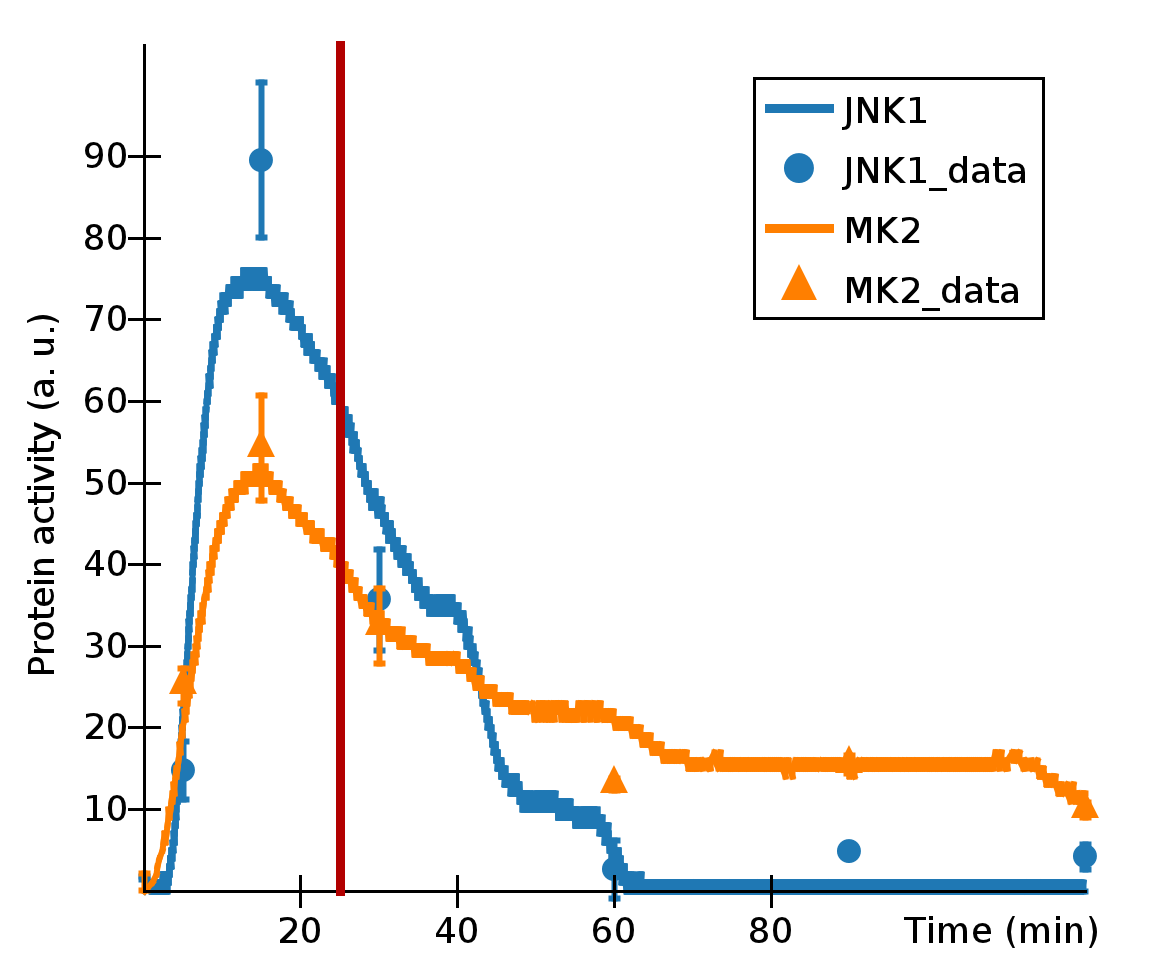
\includegraphics[scale=\halfGraphScale]{images/00-paper-graph3n_riga}}
% \subfloat[\label{fig:small-model-fourth-graph}]{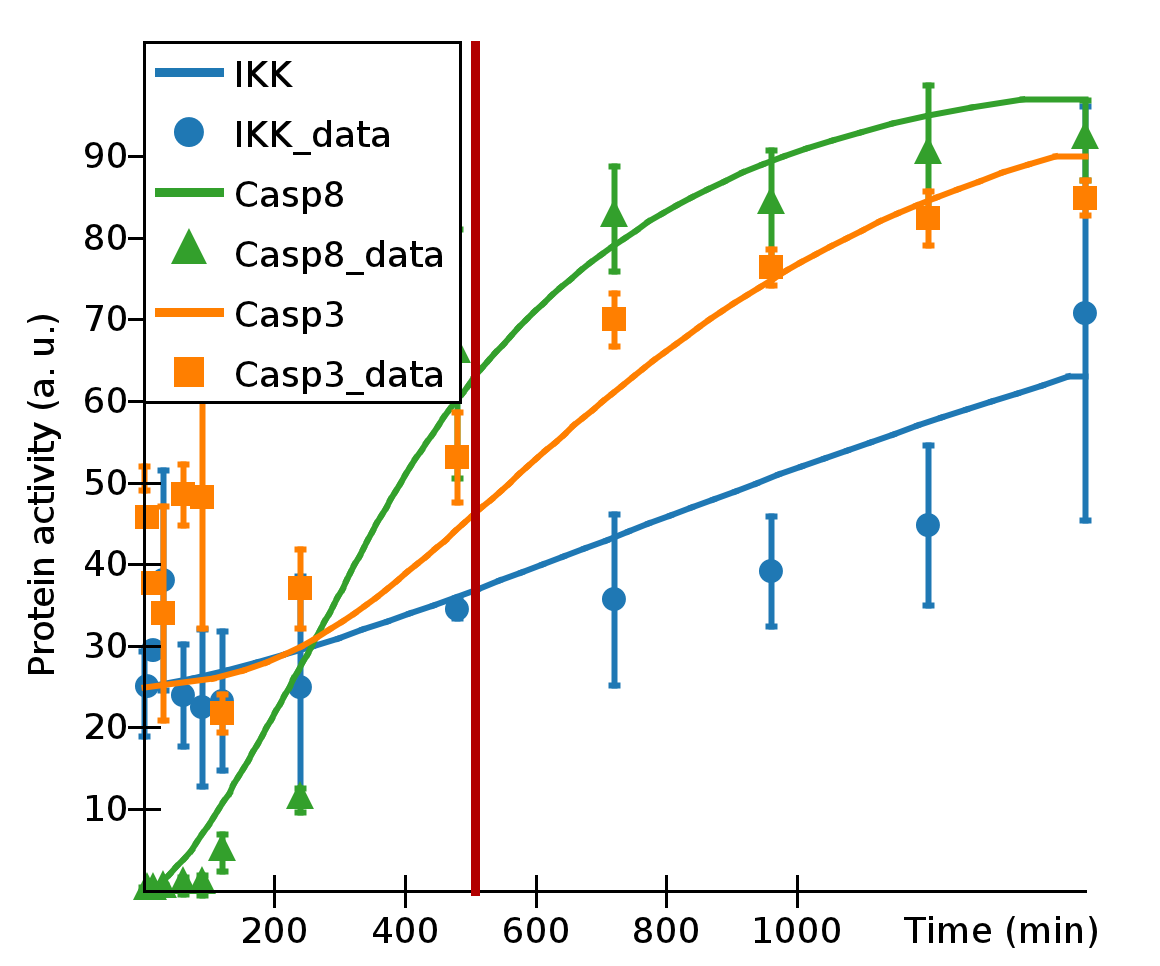
\includegraphics[scale=\halfGraphScale]{images/00-paper-graph4o_riga}}
  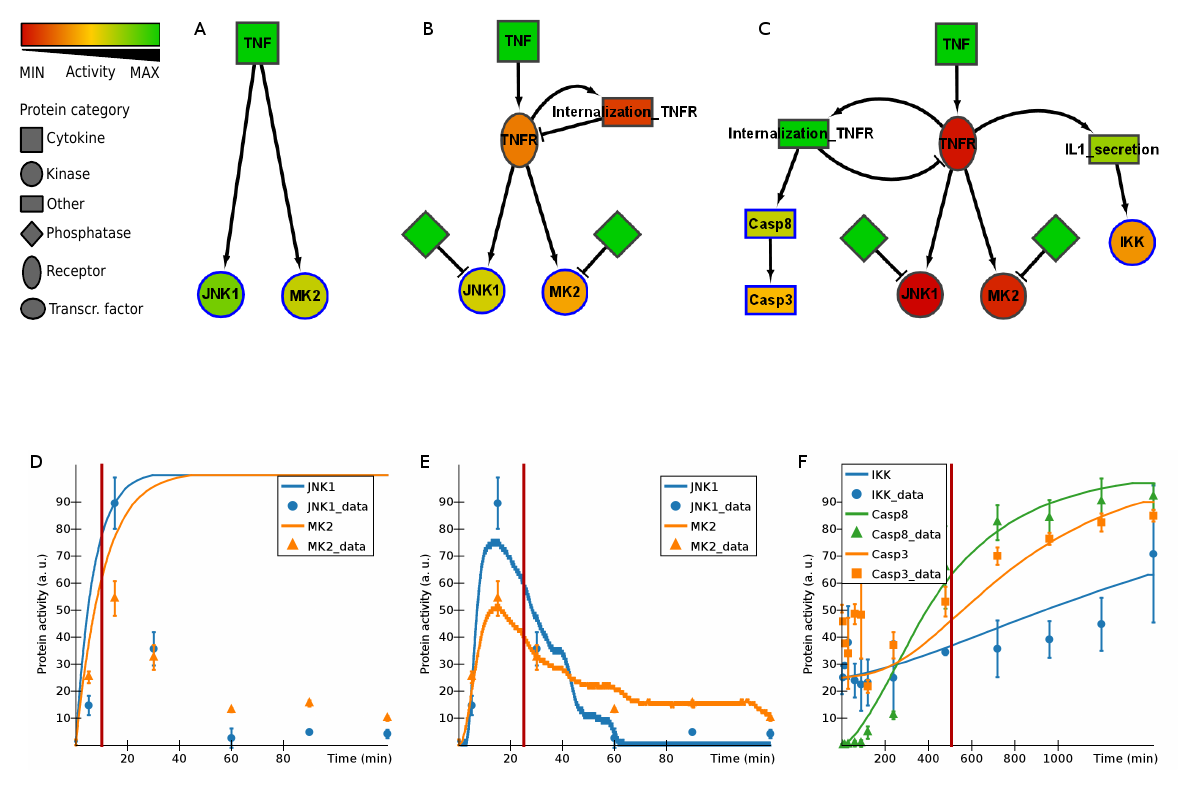
\includegraphics[width=0.9\textwidth]{images/small_model_oneImage}
  \caption{
%{\bf (\protect\subref*{subfig:mek-erk} - \protect\subref*{subfig:mek})}
%\\
%{\bf (\protect\subref*{fig:small-model-first} - \protect\subref*{fig:small-model-fourth-graph})}
\csentence{Construction of an ANIMO model of signal transduction
events in human colon carcinoma cells upon stimulation with 100 ng/ml TNF$\alpha$.}
Graphs below show the dynamic behavior of the corresponding models above, comparing it to the measured
activity values from~\cite{pathway-compendium} (error bars represent the standard deviation).
On the vertical axis, ``100'' represents the maximum protein activity in the complete experiment.
A red vertical line in each graph highlights an arbitrary time point in the time course:
nodes in the corresponding model are colored according to their activity at that time point.
{\bf(A,~D)} %{\bf (\protect\subref*{fig:small-model-first}, \protect\subref*{fig:small-model-first-graph})}~
Basic model showing direct activation of JNK1 and MK2 by TNF$\alpha$.
No peak dynamics are observed because no inactivating processes are present.
%{\bf (\protect\subref*{fig:small-model-second}, \protect\subref*{fig:small-model-second-graph})}~The model with added phosphatases.
{\bf(B,~E)} %{\bf (\protect\subref*{fig:small-model-third}, \protect\subref*{fig:small-model-third-graph})}~
The model after addition of inactivating phosphatases and a negative feedback loop that downregulates TNFR. Note that adding TNFR internalization or phosphatases alone would not be enough to reproduce activity peaks.
{\bf(C,~F)} %{\bf (\protect\subref*{fig:small-model-fourth}, \protect\subref*{fig:small-model-fourth-graph})}~
The model after addition of IKK, IL1-secretion (abstracting
the autocrine IL-1 signaling described in~\cite{pathway-autocrine}), Casp8 and Casp3, showing the late response to TNF$\alpha$ signaling.
As the data set did not contain values for cleaved caspase-3, but only for its non-cleaved precursor pro-caspase-3,
we computed the {\sf Casp3\_{}data} series as $100\% - [\mbox{\sf pro-Casp3}]$.\label{fig:small-model}}
\end{figure*}
%\end{floatingfigure}






%%%%%%%%%%%%%%%%%%%%%%%%%%%%%%%%%%%
%%                               %%
%% Tables                        %%
%%                               %%
%%%%%%%%%%%%%%%%%%%%%%%%%%%%%%%%%%%

%% Use of \listoftables is discouraged.
%%
\clearpage
\section*{Tables}
% \begin{table}[h!]
% \caption{Sample table title. This is where the description of the table should go.}
%       \begin{tabular}{cccc}
%         \hline
%            & B1  &B2   & B3\\ \hline
%         A1 & 0.1 & 0.2 & 0.3\\
%         A2 & ... & ..  & .\\
%         A3 & ..  & .   & .\\ \hline
%       \end{tabular}
% \end{table}





\newcolumntype{x}[1]{%
>{\centering\hspace{0pt}}p{#1}}%
% \savenotes
\begin{table*}[!hbt]
\begin{minipage}{\textwidth}
\begin{center}
{\scriptsize \begin{tabular}{p{3cm}p{1.2cm}p{1.1cm}p{1.2cm}p{1cm}p{1cm}p{1cm}}
\hline \ \\
{\bfseries Tool} & {\bfseries Formalism} & {\bfseries Hidden formalism} & {\bfseries Visual modeling} & {\bfseries Qualitative parameters} & {\bfseries Tight coupling with topology} & {\bfseries User-chosen granularity}  \\[5mm]
\hline \ \\
% \noalign{\vskip 2mm} 
ANIMO~\cite{animo-bibe} & Timed \ \ \ Automata & Yes & Yes & Yes & Yes & Yes
      \\[5mm]
% \noalign{\vskip 2mm}
Bio-PEPA Workbench~\cite{biopepa-interface} & Bio-PEPA & No & No & No & No & Yes
      \\[5mm]
% \noalign{\vskip 2mm}
Cell Illustrator~\cite{cell-illustrator} & Petri Nets & Yes & Yes & No & Yes & No
     \\[5mm]
% \noalign{\vskip 2mm}
COPASI~\cite{copasi} & ODE, stochastic models & No & No & No & No & No
      \\[5mm]
% \noalign{\vskip 2mm} 
COSBI LAB~$^1$
 & BlenX & Yes & Yes & No & Yes & No
      \\[5mm]
% \noalign{\vskip 2mm} 
GINsim~\cite{ginsim} & Boolean Networks & No & Yes & Yes & Yes & Yes~$^2$
      \\[5mm]
% \noalign{\vskip 2mm} 
GNA~\cite{gna}    & PLDE & No & Yes & Yes & Yes & Yes~$^2$
      \\
% \noalign{\vskip 2mm} 
Rhapsody~$^3$
 & Statecharts & No & Yes & Yes & No~$^4$ & No
      \\[5mm]
\hline \ \\
\end{tabular}}
\end{center}
\end{minipage}
\caption{Comparison between ANIMO and some existing approaches to modeling biological systems.
A ``Yes'' under a column indicates that the modeling tool (mostly) fulfills the parameter, ``No'' indicates very limited or no fulfillment.\\
$^1$ {COSBILab} web page \protect\url{http://www.cosbi.eu/index.php/research/cosbi-lab}\\
$^2$ The user can choose the number of levels for each reactant, allowing to define
multi-level models based on Boolean reaction dynamics.\\
% $^3$ When discretizing an ODE model, the granularity depends on the mathematical
% features of the model, and not directly on the user's choice.\\
$^3$ {IBM Rational Rhapsody} web page \protect\url{http://www-01.ibm.com/software/rational/products/rhapsody/designer}\\
$^4$ Statecharts represent more closely the so-called \protect\emph{transition system} of the model as opposed to the components and interactions occurring among them.
\label{tab:tool-comparison}}
\end{table*}


%%%%%%%%%%%%%%%%%%%%%%%%%%%%%%%%%%%
%%                               %%
%% Additional Files              %%
%%                               %%
%%%%%%%%%%%%%%%%%%%%%%%%%%%%%%%%%%%

\clearpage

\section*{Additional Files}
  \subsection*{Additional file 1 --- ANIMO models and data for the case studies}
      The provided .zip file contains the Cytoscape .cys network files which can be analyzed
      with ANIMO. In addition, the reference values in .csv format are provided, to compare
      ANIMO's results with the previously existing models.


\end{backmatter}


%\end{document}

\appendix
\clearpage
\setcounter{figure}{0}
\setcounter{table}{0}
\setcounter{page}{1}
\onecolumn


% \setlength{\oddsidemargin}{1.875in}
% \setlength{\evensidemargin}{1.875in}
% \addtolength{\textwidth}{-3.75in}

% \newlength\addedmarginsingle
% \setlength\addedmarginsingle{0.875in}
% \newlength\addedmargintotal
% \setlength\addedmargintotal{2\addedmarginsingle}
% 
% \addtolength{\oddsidemargin}{\addedmarginsingle}
% \addtolength{\evensidemargin}{\addedmarginsingle}
% \addtolength{\textwidth}{-\addedmargintotal}
% \addtolength{\linewidth}{-\addedmargintotal}
% \addtolength{\hsize}{-\addedmargintotal}
% \addtolength{\topmargin}{\addedmarginsingle}
% \addtolength{\textheight}{-\addedmargintotal}
% \addtolength{\vsize}{-\addedmargintotal}

\pagestyle{plain}

\clearpage
% \thispagestyle{empty}\ \

\thispagestyle{empty}
\ \\ \ \\ \ \\ \ \\ \ \\
\begin{center}
 %{\Huge Bringing biological networks}\\ \ \\ {\Huge to life with ANIMO}\\ \ \\ \ \\
 {\huge Additional Materials}
\end{center}
\clearpage






\makeatletter

% Copied from the LaTeX sources
\def\addcontentsline#1#2#3{%
  \addtocontents{#1}{\protect\contentsline{#2}{#3}{\thepage}}}
\long\def\addtocontents#1#2{%
  \protected@write\@auxout
    {\let\label\@gobble \let\index\@gobble \let\glossary\@gobble}%
    {\string\@writefile{#1}{#2}}}
\titlecontents{section} % set formatting for \section -
                        % \subsection must be formatted separately
[2.em]                 % adjust left margin
{\bf}             % font formatting
{\contentslabel{2.em}} % section label and offset
{\hspace*{-2.em}}
{\titlerule*[1pc]{}\contentspage}
\titlecontents{subsection} % set formatting for \section -
                        % \subsection must be formatted separately
[4.5em]                 % adjust left margin
{\rmfamily}             % font formatting
{\contentslabel{2.5em}} % section label and offset
{\hspace*{2.5em}}
{\titlerule*[1pc]{.}\contentspage}
% Copied from article.cls
%\setcounter{tocdepth}{5}
\renewcommand\tableofcontents{%
\begin{spacing}{1.3}
    \section*{\contentsname
        \@mkboth{%
           \MakeUppercase\contentsname}{\MakeUppercase\contentsname}}%
    \@starttoc{toc}%
\end{spacing}
}
% \newcommand*\l@paragraph{\@dottedtocline{4}{7.0em}{4.1em}}
% \newcommand*\l@subparagraph{\@dottedtocline{5}{10em}{5em}}
% \newcommand\listoffigures{%
%     \section*{\listfigurename}%
%       \@mkboth{\MakeUppercase\listfigurename}%
%               {\MakeUppercase\listfigurename}%
%     \@starttoc{lof}%
%     }
% \newcommand*\l@figure{\@dottedtocline{1}{1.5em}{2.3em}}
% \newcommand\listoftables{%
%     \section*{\listtablename}%
%       \@mkboth{%
%           \MakeUppercase\listtablename}%
%          {\MakeUppercase\listtablename}%
%     \@starttoc{lot}%
%     }
% \let\l@table\l@figure

\makeatother




\addtocontents{toc}{\protect\setcounter{tocdepth}{5}}
\thispagestyle{empty}
\tableofcontents
\clearpage

\setcounter{page}{1}
\setcounter{section}{0}

\renewcommand\figurename{Figure}
\renewcommand*\thefigure{S\arabic{figure}}
\renewcommand*\thetable{S\arabic{table}}

\def\ta{TA}
\def\tas{TA}




\clearpage
\section{Naming conventions}\label{suppl-sec:names}
Table~\ref{suppl-tab:names} explains the abbreviations used in the paper.

\begin{center}
\begin{longtable}{lll}
\caption{Explanation of the abbreviated names referring to molecular species
in the main text.}\label{suppl-tab:names} \\
%\begin{tabular}{lll}
\hline
\noalign{\vskip 2mm} {\bfseries Abbreviation} & {\bfseries Full name} \\[2mm]
\hline
\endfirsthead

\multicolumn{3}{c}%
{\scriptsize{\bfseries \tablename\ \thetable{}} \--\ continued from previous page} \\
\hline
\noalign{\vskip 2mm} {\bfseries Abbreviation} & {\bfseries Full name} \\[2mm]
\hline
\endhead

\hline \multicolumn{3}{r}{{Continued on next page}} \\ %\hline
\endfoot

\hline
\endlastfoot

\noalign{\vskip 2mm}  Akt & protein kinase B & P31749\\
\noalign{\vskip 2mm}  AP-1 & activator protein 1 & heterodimer \\
                            & & of c-Jun and c-Fos\\
\noalign{\vskip 2mm}  Casp3 & caspase 3 & P42574\\
\noalign{\vskip 2mm}  Casp8 & caspase 8 & Q14790\\
\noalign{\vskip 2mm}  c-Fos & proto-oncogene-protein c-fos & P01100\\
\noalign{\vskip 2mm}  c-Jun & Jun activation domain binding protein & P05412\\
\noalign{\vskip 2mm}  CLK & clock & O61735\\
\noalign{\vskip 2mm}  CRY & cryptochrome & O77059\\
\noalign{\vskip 2mm}  CWO & clockwork orange & Q9VGZ5\\
\noalign{\vskip 2mm}  CYC & cycle & O61734\\
\noalign{\vskip 2mm}  CYC/CLK & cycle-clock complex & \\
\noalign{\vskip 2mm}  DBT & double-time kinase & O76324\\
\noalign{\vskip 2mm}  DISC1 & death-inducing signaling complex 1 & \\
\noalign{\vskip 2mm}  DISC2 & death-inducing signaling complex 2 & \\
\noalign{\vskip 2mm}  EGF & epidermal growth factor & P01133\\
\noalign{\vskip 2mm}  EGFR & EGF receptor & P00533\\
\noalign{\vskip 2mm}  ERK & extracellular regulated kinase & P27361\\
\noalign{\vskip 2mm}  FKHR & forkhead box protein O1 & Q12778\\
\noalign{\vskip 2mm}  IKK & inhibitor of nuclear factor kappa-B kinase & O14920\\
\noalign{\vskip 2mm}  IL-1a & interleukin 1 $\alpha$ & P01583\\
\noalign{\vskip 2mm}  IL-1R & interleukin 1 receptor & P14778\\
\noalign{\vskip 2mm}  IL-1ra & interleukin 1 receptor antagonist & P18510\\
\noalign{\vskip 2mm}  IRS1 (S) & insulin receptor substrate 1 (Serine 636) & P35568\\
\noalign{\vskip 2mm}  IRS1 (Y) & insulin receptor substrate 1 (Tyrosine 896) & P35568\\
\noalign{\vskip 2mm}  JNK1 & c-Jun N-terminal kinase 1 & P45983\\
\noalign{\vskip 2mm}  MEK & MAPK ERK kinase & Q02750\\
\noalign{\vskip 2mm}  MEKK1 & MAPK/ERK kinase kinase 1 & Q13233\\
\noalign{\vskip 2mm}  MK2 & mitogen-activated protein kinase-activated protein kinase 2 & P49137\\
\noalign{\vskip 2mm}  MKK3/6 & dual specificity mitogen-activated protein kinase kinase 3/6 & P46734 / P52564\\
\noalign{\vskip 2mm}  MKK4/7 & dual specificity mitogen-activated protein kinase kinase 4/7 & P45985 / O14733\\
\noalign{\vskip 2mm}  NF-kB & nuclear factor kappa-B & P19838\\
\noalign{\vskip 2mm}  p38 & mitogen-activated protein kinase p38 & Q16539\\
\noalign{\vskip 2mm}  PDP1 & par-domain protein 1 & Q9TVY0\\
\noalign{\vskip 2mm}  PER & period & P07663\\
\noalign{\vskip 2mm}  PER/TIM-p & phosphorylated period-timeless complex & \\
\noalign{\vskip 2mm}  RAF & Raf & P04049\\
\noalign{\vskip 2mm}  RAS & Ras GTPase-activating protein & P01112\\
\noalign{\vskip 2mm}  TGF$\alpha$ & transforming growth factor $\alpha$ & P01135\\
\noalign{\vskip 2mm}  TNF$\alpha$ & tumor necrosis factor-$\alpha$ & P01375\\
\noalign{\vskip 2mm}  TNFR & TNF receptor & P19438\\
\noalign{\vskip 2mm}  TIM & timeless & P49021\\
\noalign{\vskip 2mm}  VRI & vrille & O18660\\[2mm]
\hline
%\end{tabular}
\end{longtable}
\end{center}




\clearpage
\section{Normalizing experimental data for use with ANIMO}\label{suppl-sec:normalization}
Document S1 in the Supplemental Data of~\cite{pathway-autocrine} contains
three tables, named {\sf Replicates}, {\sf Averages} and {\sf DPLSR dataset}.
The data we use to compare the results computed with ANIMO are based on the
values from the {\sf Averages} table.
In particular, we compute activity data by performing a normalization on a $0\dots 100$ scale using this formula
$$
v_{\mbox{\scriptsize norm}} = \frac{v}{v_{\mbox{\scriptsize max}}} \times 100
$$
where $v$ is the datum to be normalized taken from the column $v$ in the {\sf Averages} table,
$v_{\mbox{\scriptsize norm}}$ is the normalized value and
$v_{\mbox{\scriptsize max}}$ is the maximum value over the whole column $v$ in the {\sf Replicates} table.
For each series, we compute also the standard deviation using the triplicate measurements
present in table {\sf Replicates}. The standard deviation is also normalized using the formula presented for the average.
Each table produced with this process contains a subset of the columns from the {\sf Averages} table,
and refers to one treatment condition only. A column with time references is added to the table in first position.
Finally, a column named \emph{Number\_of\_levels} containing only the value $100$ (see the instructions
on page~\pageref{csv-import-format}) is added at the rightmost position.
The tables are all exported in .csv format to be used with ANIMO, and are included in the \emph{Model\_and\_data.zip}
file in the additional materials of the present work.


\clearpage
\section{ANIMO and Timed Automata}\label{suppl-sec:animo-ta}
\subsection{Modeling abstractions}\label{subsec:abstractions}

In living cells, cascades of chemical and physical interactions enable propagation of signals through molecular networks.
In this process, the activity of upstream molecules induces a change in the 
concentration or activity of downstream molecules. For many reactions, the values of the kinetic parameters 
are unknown or difficult to collect. This lack of knowledge hampers the feasibility 
of computational models that describe molecular networks in fine mechanistic detail, especially for larger networks.
As a solution to this problem, we propose the construction of models at a higher level of abstraction, 
thereby reducing the number of parameters involved. In choosing a suitable abstraction level, it is important to 
retain enough descriptive power to give a meaningful formal description of the topology and the 
associated dynamic behavior of biological networks.

As a first abstraction in ANIMO models, the active and inactive forms of each network component 
are represented together by a single node in the network.
Each of these nodes is characterized by its \emph{activity level}, which
represents the fraction of active molecules of that molecular species. When a molecule is known to be 
constitutively active, changes in concentrations of that molecule are treated as changes in its activity level.
Activity levels are discretized into integer variables with a user-defined granularity, ranging from 
Boolean (2 levels) to near-continuous (100 levels).

Detailed biochemical reaction mechanisms are abstracted to \emph{interactions}, which can 
represent either activations ($\rightarrow$) or inhibitions ($\dashv$\hspace{0.1em}). 
This aggregation of elementary reactions into single interaction steps reduces the number of kinetic 
parameters involved, while preserving cause-and-effect relationships.
For example, consider a reaction in which enzyme $E$ phosphorylates and activates substrate $S$, 
transferring a phosphate group from a molecule of ATP to a molecule of $S$. Biochemically, this reaction 
can be represented as
$$
\mbox{\it E} + \mbox{\it S} + \mbox{\it ATP} \rightleftarrows \mbox{\it ES} + \mbox{\it ATP} \rightarrow \mbox{\it ES}^{\mbox{\scriptsize \it P}} + \mbox{\it ADP} \rightleftarrows \mbox{\it E} + \mbox{\it S}^{\mbox{\scriptsize\it P}} + \mbox{\it ADP},
$$
with conservation condition $\mbox{\it S} + \mbox{\it S}^{\mbox{\scriptsize\it P}} = \mbox{constant}$ and $\mbox{\it ATP} + \mbox{\it ADP} = \mbox{constant}$.\\
Under the assumption of ATP constantly being replenished by the cell, this reaction is abstracted in ANIMO to the corresponding interaction
$$
\mbox{\it E} \rightarrow \mbox{\it S}.
$$
Each occurrence of the interaction $E \rightarrow S$ will increase the activity level of $S$ by one discrete step. 
Since the activity level is defined as the active fraction of a molecular species, an increase in the active fraction
implies a decrease in the inactive fraction. Hence, the original conservation condition is automatically  
satisfied.
The interaction rate, $R$, depends on the activity levels of the reactants involved and on a single kinetic
parameter $k$ that is set by the user. 
The three available interaction scenarios can be interpreted as abstracted kinetic rate laws:
\begin{enumerate}
  \item $R = k \times [E]$: the interaction rate depends only on the activity level of the upstream node.
  \item $R = k \times [E] \times [1 - S]$ (activations) or $R = k \times [E] \times [S]$ (inhibitions): the rate 
  depends on the activity levels of both the upstream and downstream participants. Activations depend on the 
  presence of inactive substrate, \emph{[1 - S]}, whereas inhibitions depend on the level of active substrate,
  \emph{[S]}.
  \item $R = k \times [E_1] \times [E_2]$: this scenario can be used when the activation or inhibition
  of a downstream node depends on the simultaneous activity of two upstream nodes. This scenario is comparable to an
  \emph{AND-gate} in Boolean logic.
\end{enumerate}
We will show in Section~\ref{sec:results} that the abstraction proposed here preserves ample
expressivity to capture the dynamic behavior of a biological network. 









\subsection{ANIMO}
The modeling approach described in Section~\ref{subsec:abstractions} and Section~\ref{subsec:timed-automata}
is implemented in the
software tool ANIMO (Analysis of Networks with Interactive MOdeling, \cite{animo-ieee}) as
a plug-in to the network visualization tool Cytoscape~\cite{cytoscape}. The visual interface of Cytoscape
makes the construction, expansion and rewiring of a network topology a fast and user-friendly process. 

When a new node is added to the network, it has to be initialized with the number of activity levels and 
its initial activity. 
For each interaction, a scenario needs to be selected, together with the corresponding kinetic parameter and 
the interaction type: activation or inhibition. All settings can be readily adapted by double clicking, or via a 
table of nodes or interactions. 

ANIMO automatically translates the user input to a \tas\ model, which is then simulated with the model 
checking tool UPPAAL~\cite{uppaal}. The results are subsequently parsed and translated to a graph that shows
the dynamic behavior of nodes in the network. 
A schematic overview of this process is given in Supplementary Section~\ref{suppl-sec:animo-ta}.
No training or prior knowledge on the use of \tas\ or UPPAAL is needed in order to benefit from ANIMO.
Nevertheless, the \tas\ model and the model checking process in UPPAAL can be accessed when desired by the user.

The dynamic behavior of a model can be interactively explored by
moving a time slider underneath the graph to highlight time points in a simulation. In the network view,
each node will be colored according to its activity level at the selected time point. 
Experimental data can be compared to the model by importing and superposing these data 
upon an output graph from the model (Figure~\ref{fig:small-model} B,D,F). The ANIMO user workflow and the 
features described above are illustrated in Suppl. Video 1.


% 
% \subsection*{Using ANIMO to build a model based on data}\label{subsec:case-study}
% To illustrate the process of modelling with ANIMO, we show the construction of a small model based on a 
% literature compendium of signal transduction events in HT-29 human colon carcinoma cells~\cite{pathway-compendium}. 
% This data set comprises triplicate
% measurements of 11 different protein activities or post-translational modification states at 13 time points after
% treatment with different combinations of TNF$\alpha$, EGF and insulin.
% The data set contains relative protein levels and activities, which is a typical situation in biochemistry.
% 
% As a first step, we normalized measurements for each protein to the
% maximum value in the complete experiment. This normalization results in a nondimensionalized data set that 
% is suitable for use with ANIMO.
% 
% In Figure~\ref{fig:small-model}, we show the stepwise construction of a model of a small part of the network that is
% able to account for measured variations in activity of IKK, JNK1, MK2, Casp8 and Casp3 upon stimulation with 100~ng/ml TNF$\alpha$.
% In this example we aimed for inclusion of a minimum number of nodes in the network, 
% while preserving biological relationships.
% Multi-step cascades were aggregated into a single step when possible. Parameters for all interactions were 
% set manually, and a close match was obtained between the model and the patterns that are present in the dataset.
% 
% A more comprehensive model based on the same dataset is presented in Section~\ref{subsec:case-study-larger}.




\subsection{Timed Automata model}
The Timed Automata (\tas) model underlying an ANIMO network is generated whenever an analysis is requested by the user.
Starting from the network represented in the Cytoscape-based user interface, ANIMO automatically generates a \tas\ model
to be used with UPPAAL. The analysis result is then parsed and properly presented to the user, for example
as a graph of reactant activity levels. This workflow is described in Figure~\ref{fig:animo-sim-workflow}.

\begin{figure}[htb]
\begin{minipage}{\textwidth}
  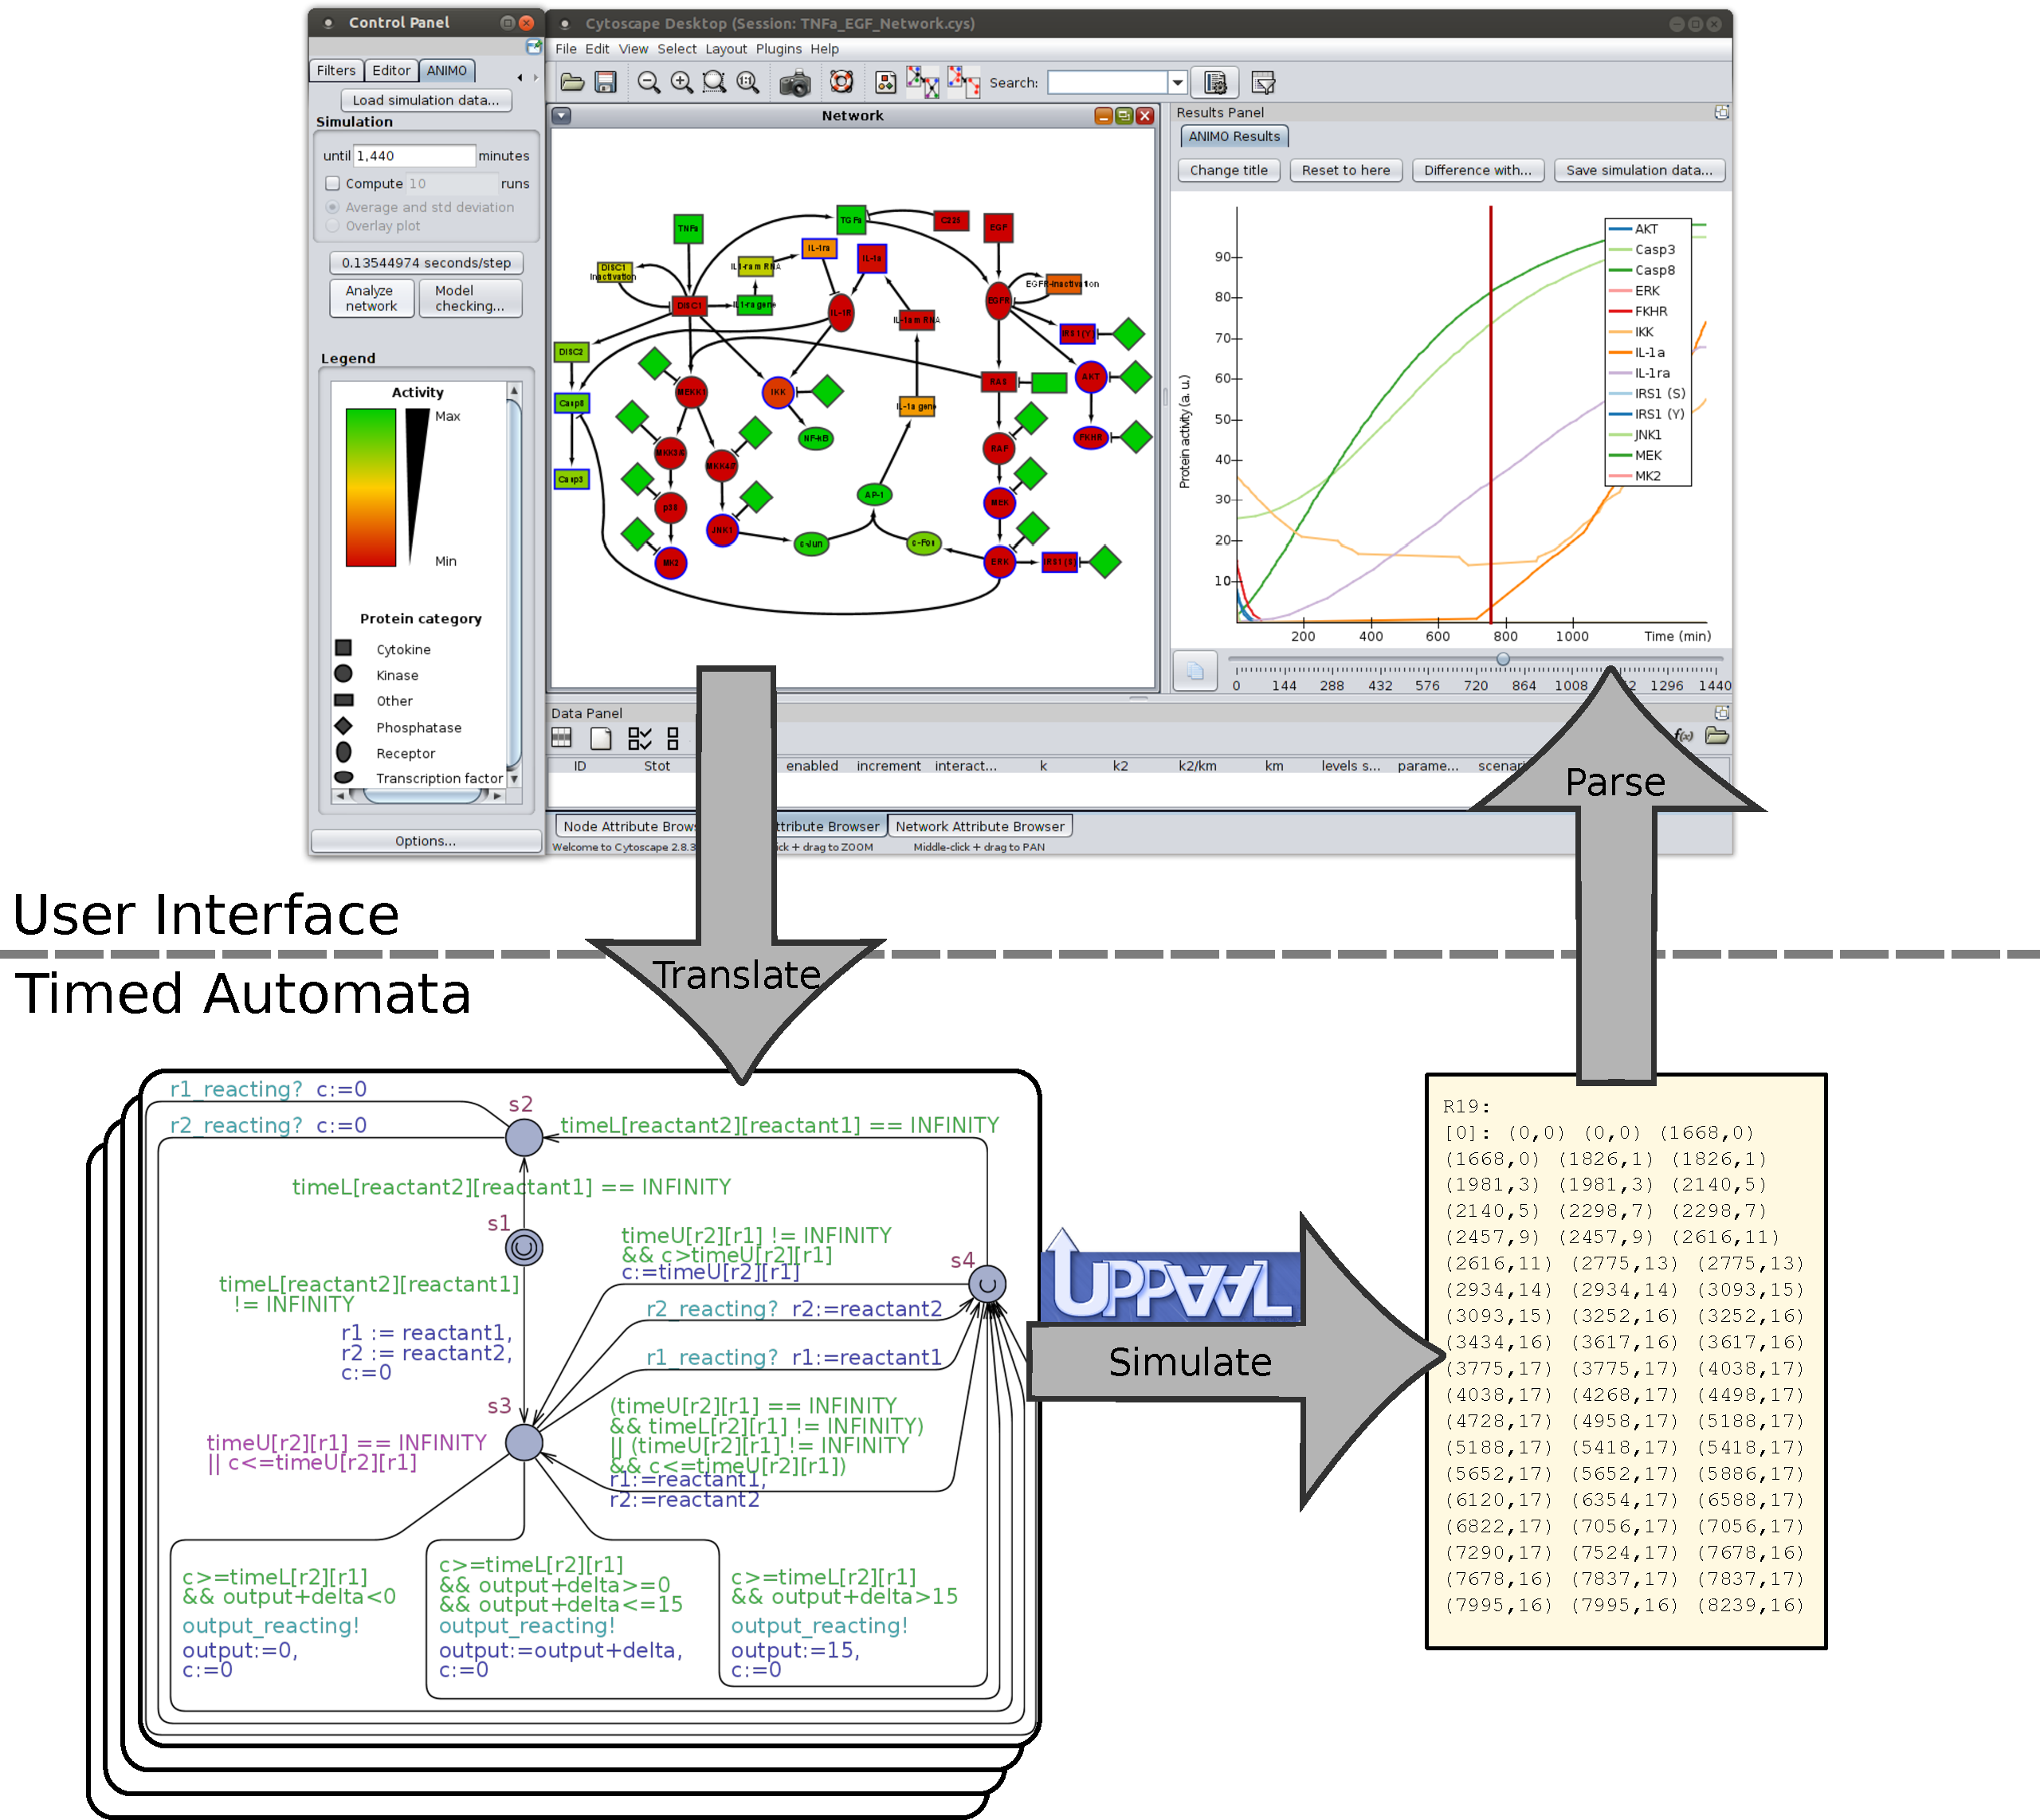
\includegraphics[width=\textwidth]{images/animo_simulation_workflow}
\caption{The passages intercurring between the press of the \emph{Analyze network} button
and the generation of an activity level graph.
A simulation produces, for each selected node, a series of pairs {\sf ($t$, $a$)},
with $t$ a time instant along the simulation and $a$ an activity level. These data are
then parsed and translated into a graph.}\label{fig:animo-sim-workflow}
\end{minipage}
\end{figure}

Each \tas\ model generated by ANIMO contains one automaton for each interaction (activation or inhibition) in the network.
A \ta\ representing an interaction performs a cyclic series of steps, continuously updating
the target of the interaction it represents, and adapting the timing of the next update according to
the user-defined dynamics. Synchronizations between different automata occur when the activity level of a network component (e.g. ERK)
changes: this allows the automata depending on that component to update their time settings.

The abstract behavior of the interaction $\mbox{MEK} \rightarrow \mbox{ERK}$ in the \tas\ model used in ANIMO is described in Figure~\ref{fig:ta-diagram}.
There, the activity levels of MEK and ERK are represented by variables called, respectively, $\mbox{MEK}_{\mbox{\scriptsize activity}}$
and $\mbox{ERK}_{\mbox{\scriptsize activity}}$. A more detailed description of the \tas\ model underlying ANIMO was
presented in the IEEE Journal of Biomedical and Health Informatics~\cite{animo-ieee}.

\tikzstyle{decision} = [rectangle, draw, fill=yellow!20, text width=.45\textwidth, text badly centered]
\tikzstyle{block} = [rectangle, draw, fill=blue!20,
    text width=.45\textwidth, text centered, rounded corners, minimum height=4em]
\tikzstyle{line} = [draw, thick, -latex']
\tikzstyle{cloud} = [draw, ellipse,fill=blue!20, minimum height=2em]
\def\svgwidth{.8\textwidth}
\definecolor{lowActivity}{rgb}{0.8,0,0}
\definecolor{highActivity}{rgb}{0,0.8,0}%{1,0.8,0}
\newsavebox{\mysquareLow}
\savebox{\mysquareLow}{%
  \raisebox{-0.08em}{%
    \textcolor{black}{%
      \rule{.7em}{.7em}%
    }%
    \hspace{-.65em}%
    \raisebox{.05em}{%
      \textcolor{lowActivity}{%
	\rule{.6em}{.6em}%
      }%
    }%
  }%
}
\newsavebox{\mysquareHigh}
\savebox{\mysquareHigh}{%
  \raisebox{-0.08em}{%
    \textcolor{black}{%
      \rule{.7em}{.7em}%
    }%
    \hspace{-.65em}%
    \raisebox{.05em}{%
      \textcolor{highActivity}{%
	\rule{.6em}{.6em}%
      }%
    }%
  }%
}

\begin{figure}[!ht]
\begin{minipage}{\textwidth}
\centering

\begin{tikzpicture}[node distance = 2cm, auto, scale=0.8, every node/.style={scale=0.8}]
    % Place nodes
    \node [block] (init) {
\begingroup
  \makeatletter
  \providecommand\color[2][]{%
    \errmessage{(Inkscape) Color is used for the text in Inkscape, but the package 'color.sty' is not loaded}
    \renewcommand\color[2][]{}%
  }
  \providecommand\transparent[1]{%
    \errmessage{(Inkscape) Transparency is used (non-zero) for the text in Inkscape, but the package 'transparent.sty'
is not loaded}
    \renewcommand\transparent[1]{}%
  }
  \providecommand\rotatebox[2]{#2}
  \ifx\svgwidth\undefined
    \setlength{\unitlength}{1974.66679688pt}
  \else
    \setlength{\unitlength}{\svgwidth}
  \fi
  \global\let\svgwidth\undefined
  \makeatother
  \begin{picture}(1,0.37)%26031697)%
    \put(0,0){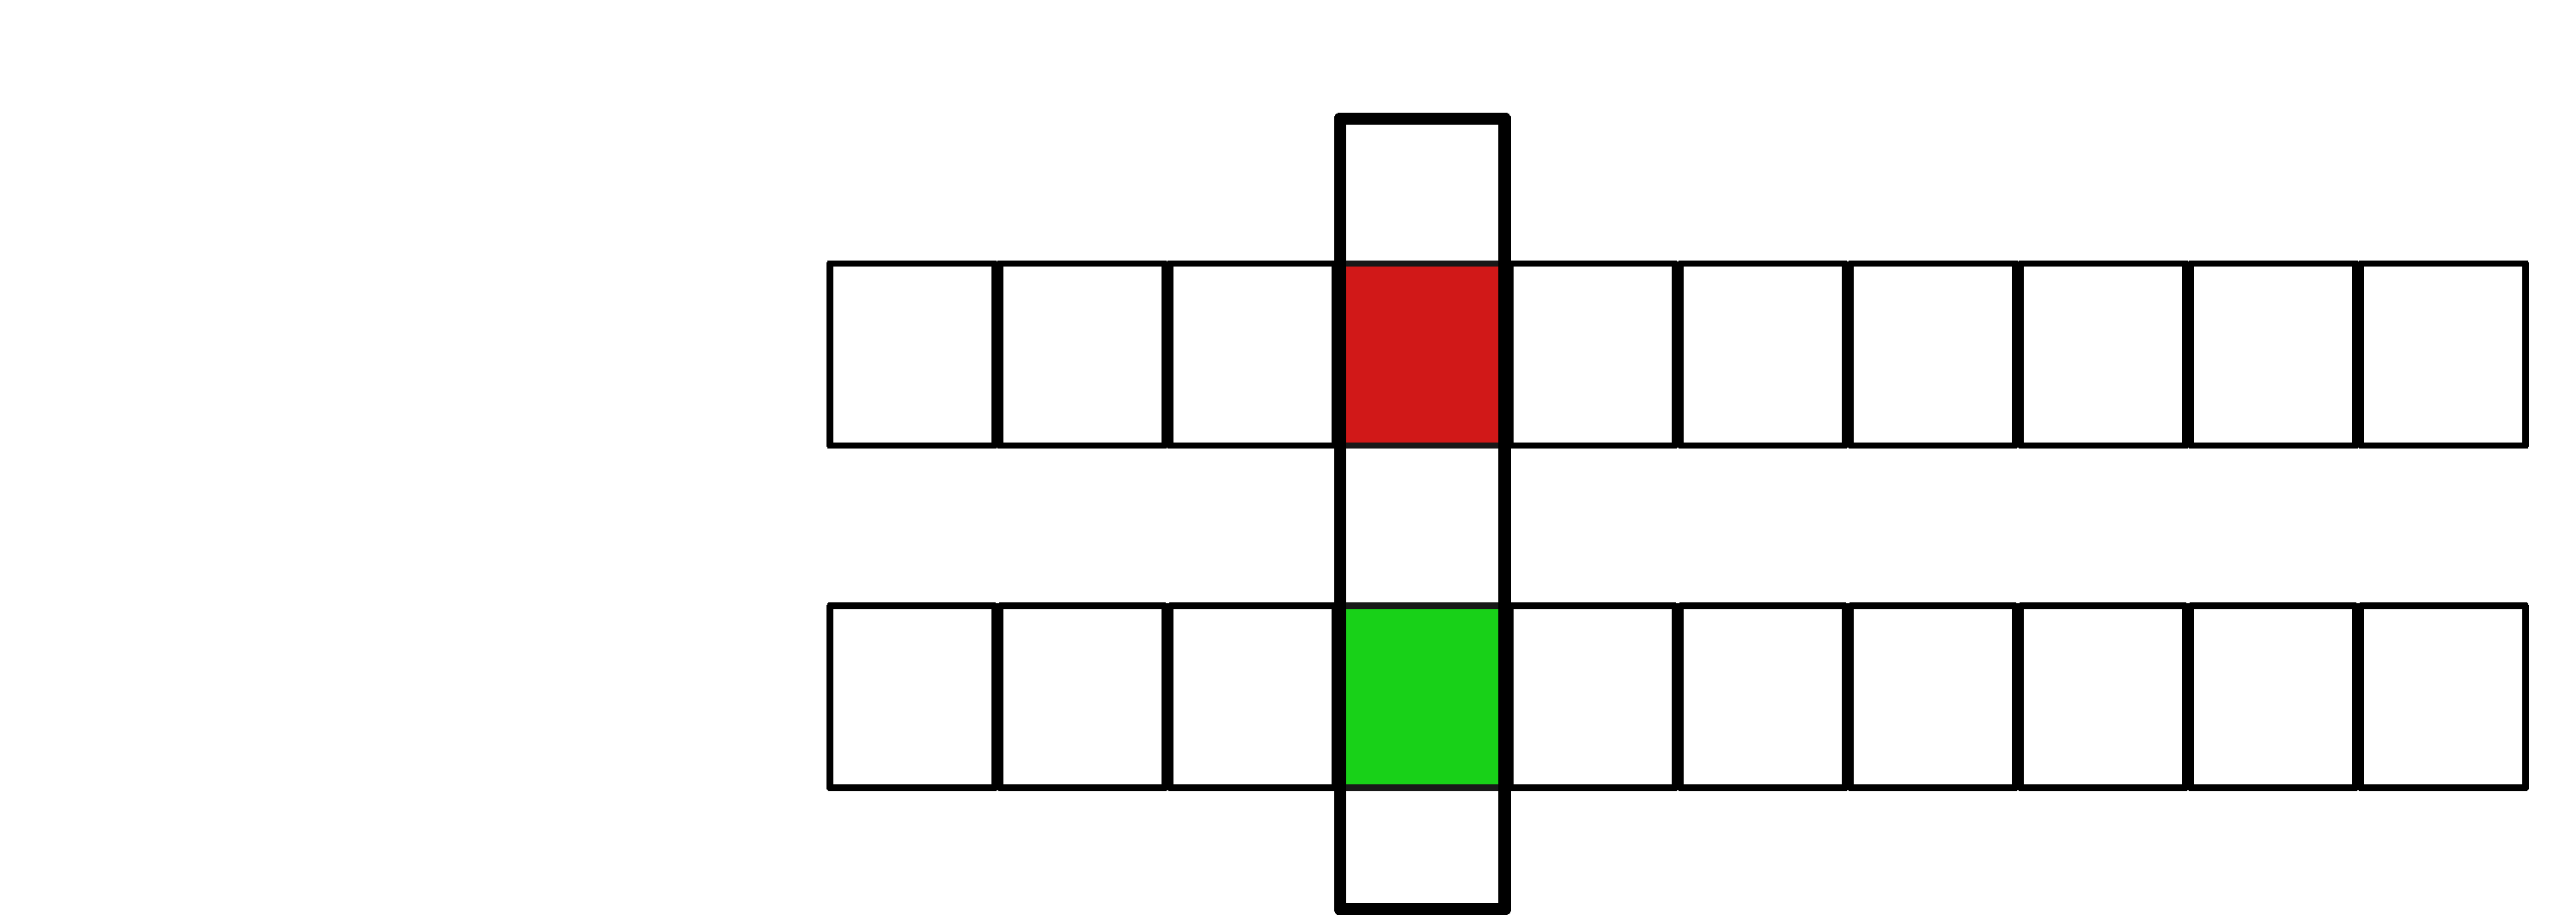
\includegraphics[width=\unitlength]{images/mek_activity_time_tables2.pdf}}%
    \put(0.005,0.20182345){\color[rgb]{0,0,0}\makebox(0,0)[lb]{\smash{$R_{\mbox{\scriptsize lowerBound}}$}}}%
    \put(0.005,0.07442319){\color[rgb]{0,0,0}\makebox(0,0)[lb]{\smash{$R_{\mbox{\scriptsize upperBound}}$}}}%
    \put(0.45,0.325)%23815501)
	{\color[rgb]{0,0,0}\makebox(0,0)[lb]{\smash{$\mbox{MEK}_{\mbox{\scriptsize
activity}}$}}}%
  \end{picture}%
\endgroup
};
    \node [block, above of=init, node distance=2.5cm] (reset) {Reset the internal clock: ${\sf t} \!\!:= \!\!0$};
    \node [cloud, above of=reset, node distance=1.5cm] (start) {Start};
\node [block, below of=init, node distance=2.5cm] (choose) {$R$ will occur when
\raisebox{-0.3ex}{\pgfuseimage{lower-bound}} $\leq\!\!\! {\sf t}\!\!\! \leq$
\raisebox{-0.3ex}{\pgfuseimage{upper-bound}}
    };
    \node [block, below of=choose] (increase) {Increase $\mbox{ERK}_{\mbox{\scriptsize activity}}$
by $+1$ level};
    \node [block, below of=increase] (inform) {Inform interactions depending on $\mbox{ERK}_{\mbox{\scriptsize
activity}}$\\
    of the change};
    % Draw edges
    \path [line] (start) -- (reset);
    \path [line] (reset) -- (init);
    \path [line] (init) -- (choose);
    \path [line] (choose.west) -| +(-0.5, 2) node [pos=0.78, sloped, above, align=left] {$\mbox{MEK}_{\mbox{\scriptsize activity}}$ was changed} |- (init.west);
    \path [line] (choose) -- (increase);
    \path [line] (increase) -- (inform);
    \path [line] (inform.east) -| +(1, 4) |- (reset.east);
\end{tikzpicture}
\caption{Schematic overview of the steps taken during a simulation run by a Timed Automaton modeling an interaction $R$ that
increases $\mbox{ERK}_{\mbox{\scriptsize activity}}$ and depends only on $\mbox{MEK}_{\mbox{\scriptsize activity}}$.
In this example, MEK has 10 activity levels.\\
After resetting the internal clock {\sf t}, the automaton sets the time constraints for the interaction.
$\mbox{MEK}_{\mbox{\scriptsize activity}}$ is used as the index inside the time
tables $R_{\mbox{\scriptsize lowerBound}}$ and $R_{\mbox{\scriptsize upperBound}}$, which contain pre-computed lower- and upper-bounds
for the interaction timing.
Once the bounds have been identified, %the internal clock {\sf t} begins counting.
$R$ can occur when {\sf t} reaches a value
inside the continuous time interval~$[\,\usebox{\mysquareLow}, \usebox{\mysquareHigh}\,]$. When it occurs, $R$ increases the value of
$\mbox{ERK}_{\mbox{\scriptsize activity}}$ by $1$. All interactions that depend on
$\mbox{ERK}_{\mbox{\scriptsize activity}}$ are notified of the change (via a synchronization on a specific channel),
so that the associated time bounds are updated accordingly.
After resetting the clock {\sf t}, the process can restart.
If $\mbox{MEK}_{\mbox{\scriptsize activity}}$ was changed by another automaton before the occurrence of $R$,
the time bounds are updated according to the new activity level of MEK.}\label{fig:ta-diagram}
\end{minipage}
\end{figure}



\subsection{Granularity of an ANIMO network node}
Figure~\ref{fig:levels} shows the differences between different choices for the
number of levels of a node. This allows to adapt a model to the quality of experimental data.

\begin{figure}[htpb]
\begin{minipage}{\textwidth}
\centering
\subfloat[\label{suppl:fig1-1level}]{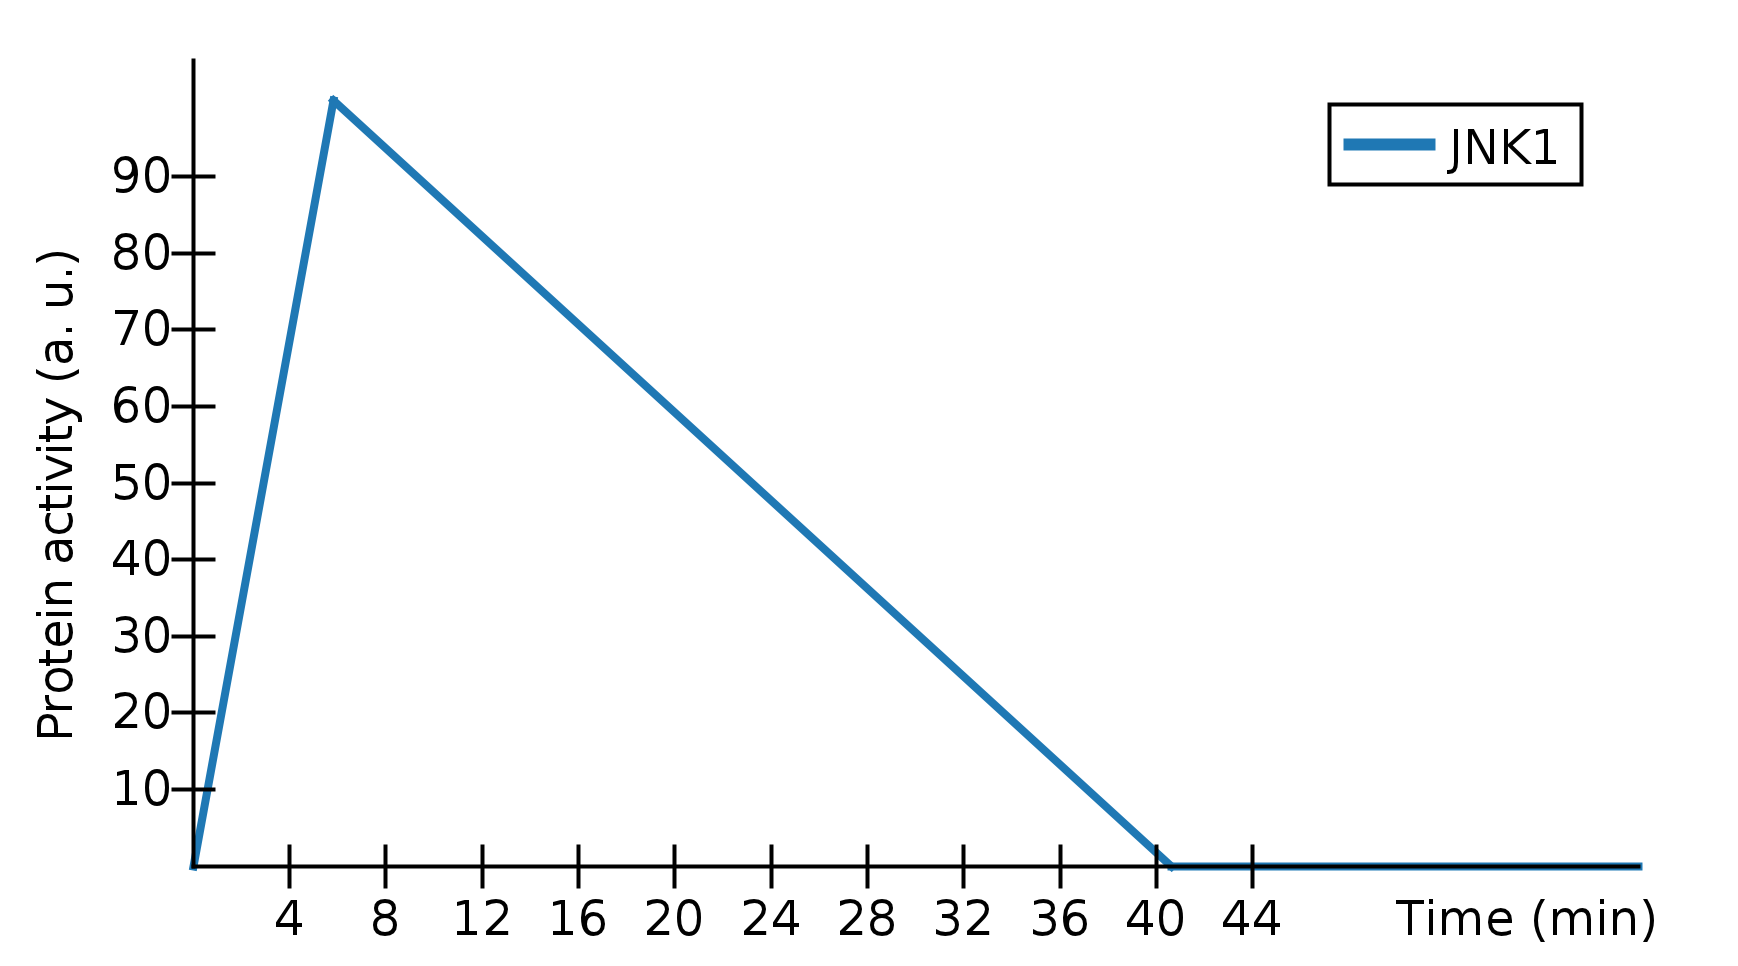
\includegraphics[width=.45\textwidth]{images/JNK1_1level2}} \qquad
\subfloat[\label{suppl:fig1-10levels}]{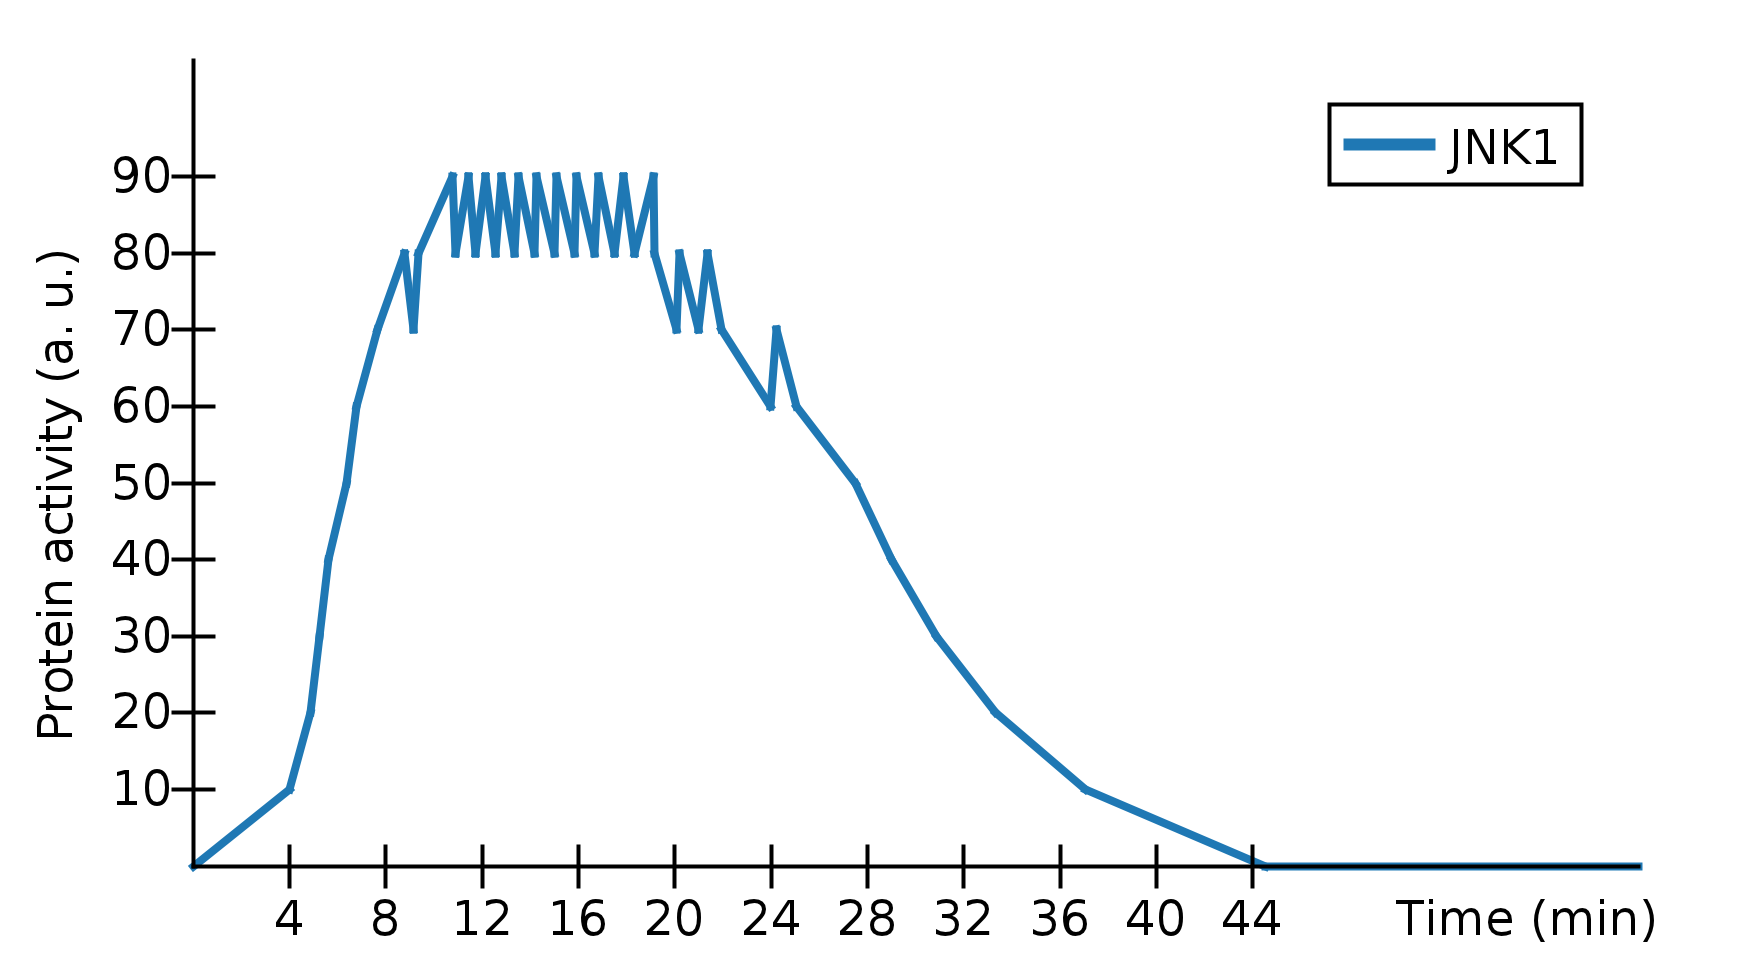
\includegraphics[width=.45\textwidth]{images/JNK1_10levels2}} \\
\subfloat[\label{suppl:fig1-50levels}]{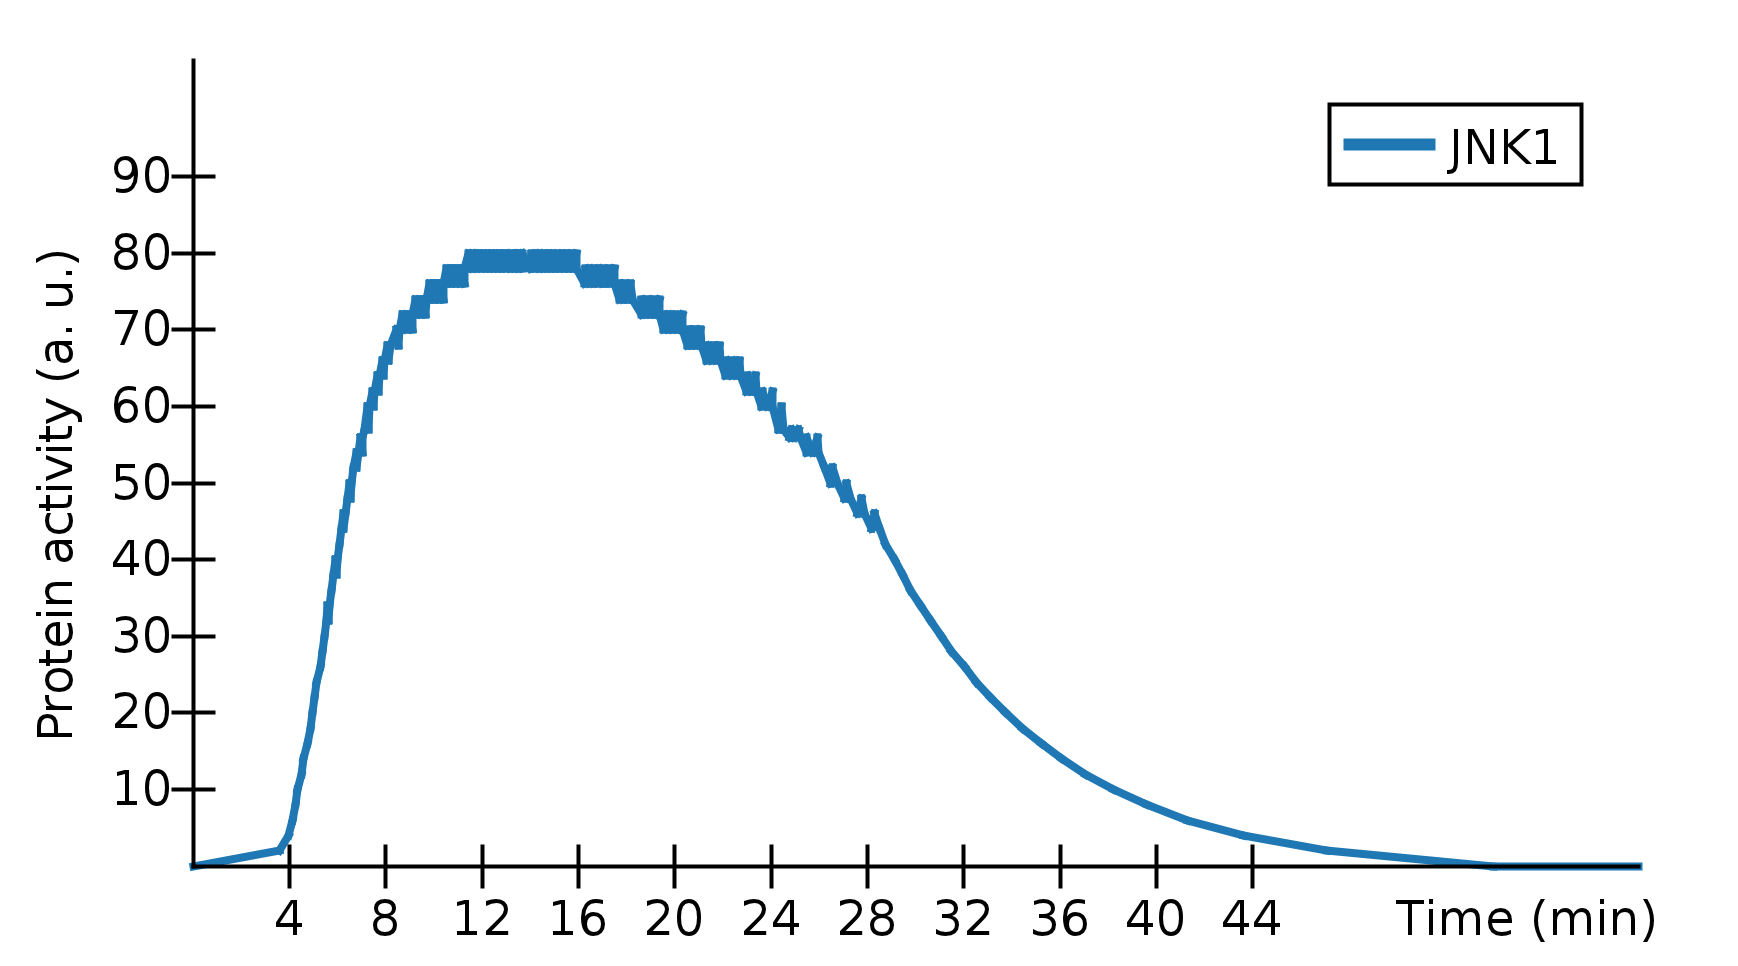
\includegraphics[width=.45\textwidth]{images/JNK1_50levels2}} \qquad
\subfloat[\label{suppl:fig1-100levels}]{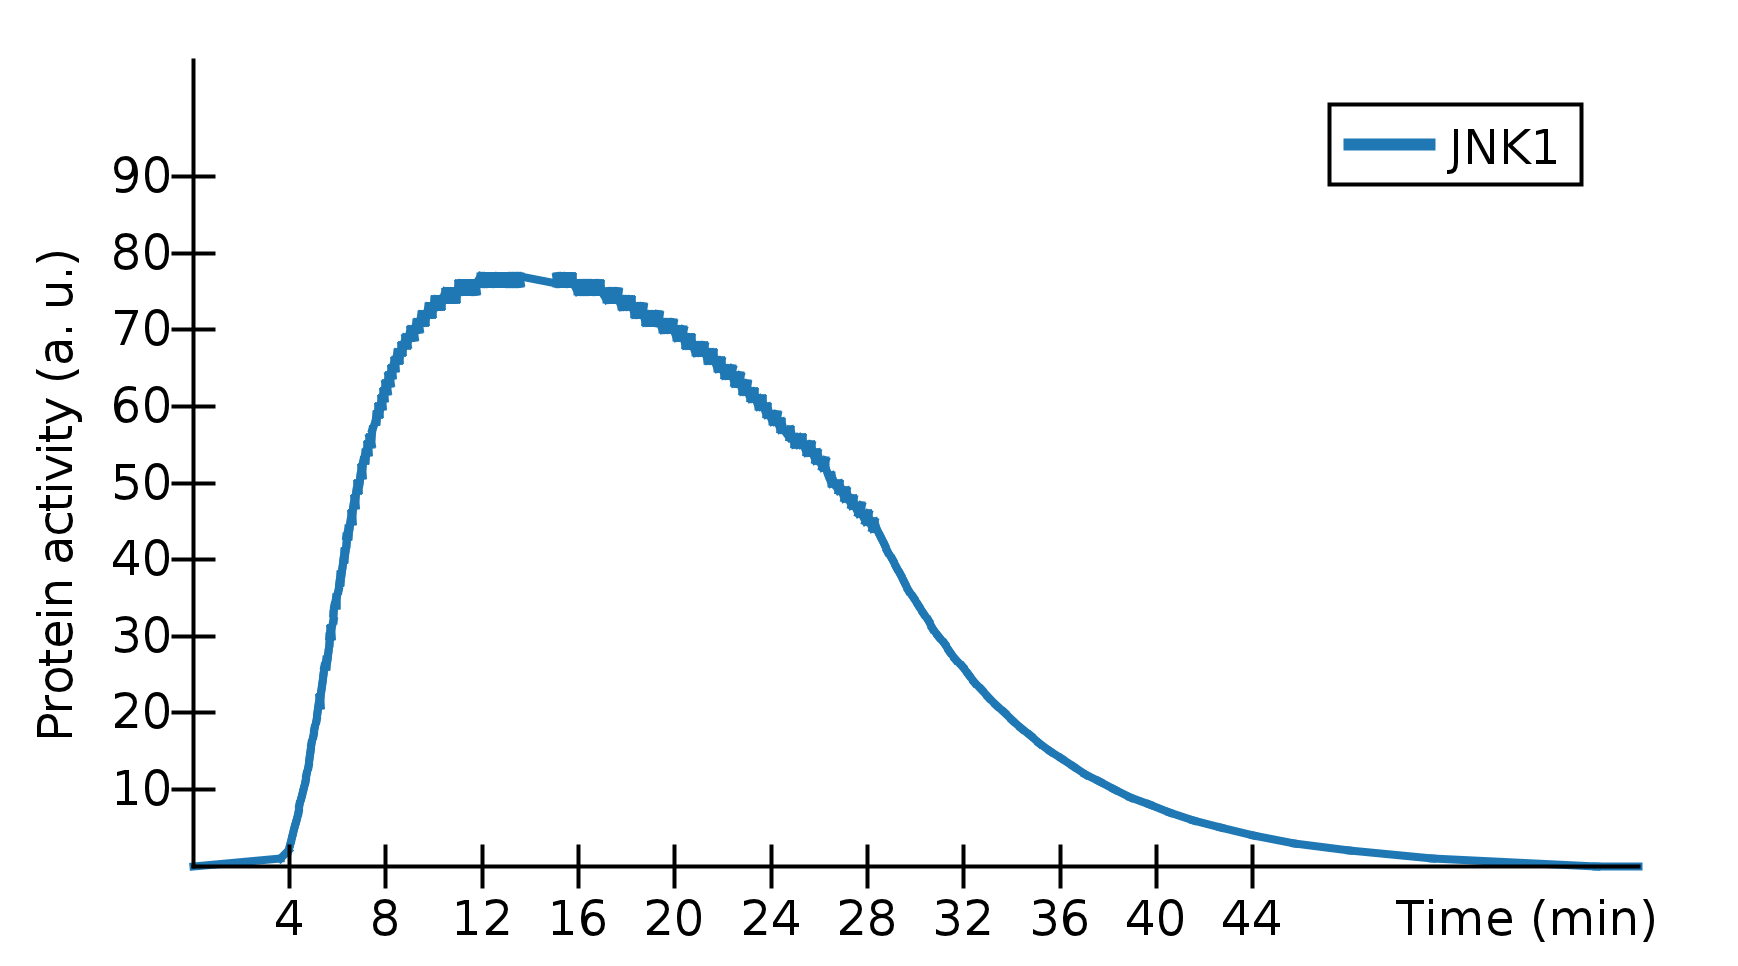
\includegraphics[width=.45\textwidth]{images/JNK1_100levels2}}
\caption{Comparing different reactant granularity settings. {\bfseries (\protect\subref*{suppl:fig1-1level})} 2 levels, {\bfseries (\protect\subref*{suppl:fig1-10levels})} 10 levels,  {\bfseries (\protect\subref*{suppl:fig1-50levels})} 50 levels, {\bfseries (\protect\subref*{suppl:fig1-100levels})} 100 levels. The {\sf JNK1} series is computed from the model presented in Figure~\ref{fig:large-model-complete}, considering 100 ng/ml TNF$\alpha$ as treatment condition over a period of 60 minutes.}\label{fig:levels}
\end{minipage}
\end{figure}



\clearpage
\section{Additional notes}

\subsection{Simulating the day-night cycle}\label{suppl:repressilator}
The model presented in Figure~\ref{fig:drosophila-model} contains a node
labeled {\sf Day/Night}. That node abstracts our representation
of the cyclic alternation of day and night, which causes the variations
in cryptochrome ({\sf cry}): these oscillations allow the network
to synchronize to a time zone. Note that the network oscillates
also when the node {\sf cry} is not included in the model.

The alternation between day and night is represented in our model with a
repressilator-like~\cite{repressilator} subnetwork, as can be seen in Figure~\ref{fig:repressilator}.
In the model in~\cite{drosophila-ode-model} a specific function
was introduced in the equations to approximate the experimental data from~\cite{drosophila-cry-data}.

\def\reprGraph{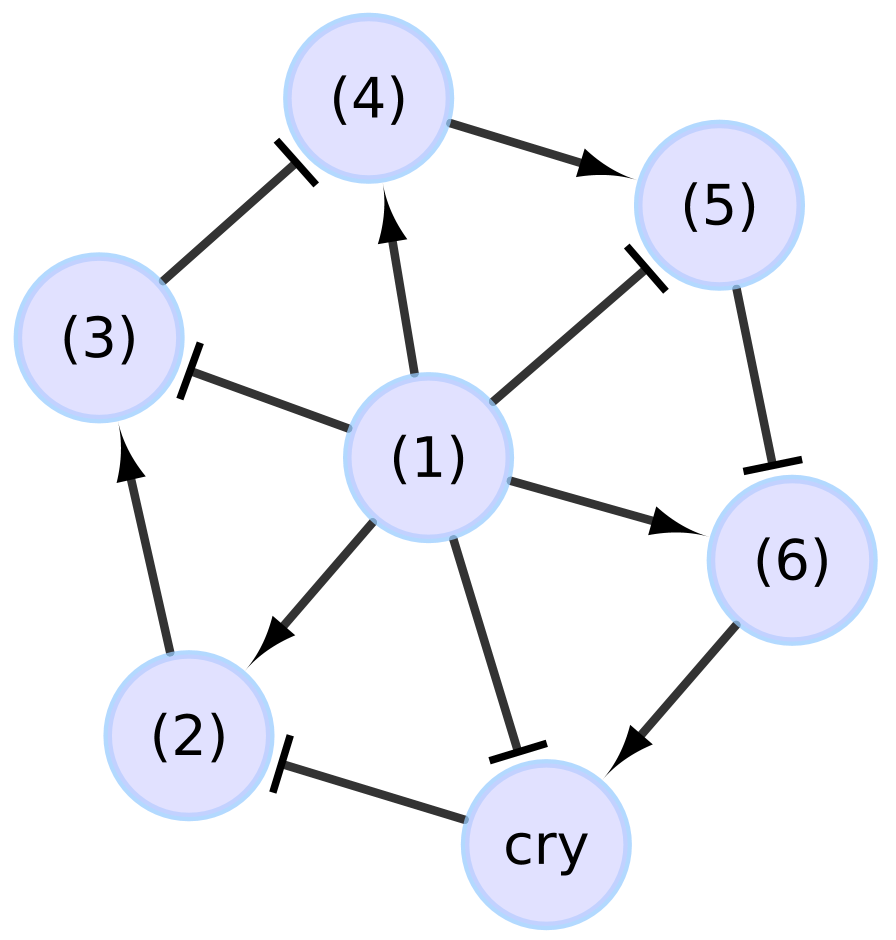
\includegraphics[scale=0.15]{images/drosophila_model_repressilator}}
\newlength\reprGraphHeight
\setlength\reprGraphHeight{\heightof{\reprGraph}}
\begin{figure}[!htb]
\begin{minipage}{\textwidth}
  \centering
  \subfloat[\label{subfig:repressilator-model}]{\begin{minipage}[c][\reprGraphHeight]{0.35\textwidth}\begin{center}\reprGraph\end{center}\end{minipage}}\qquad
  \subfloat[\label{subfig:repressilator-graph}]{\begin{minipage}[c][\reprGraphHeight]{0.6\textwidth}\begin{center}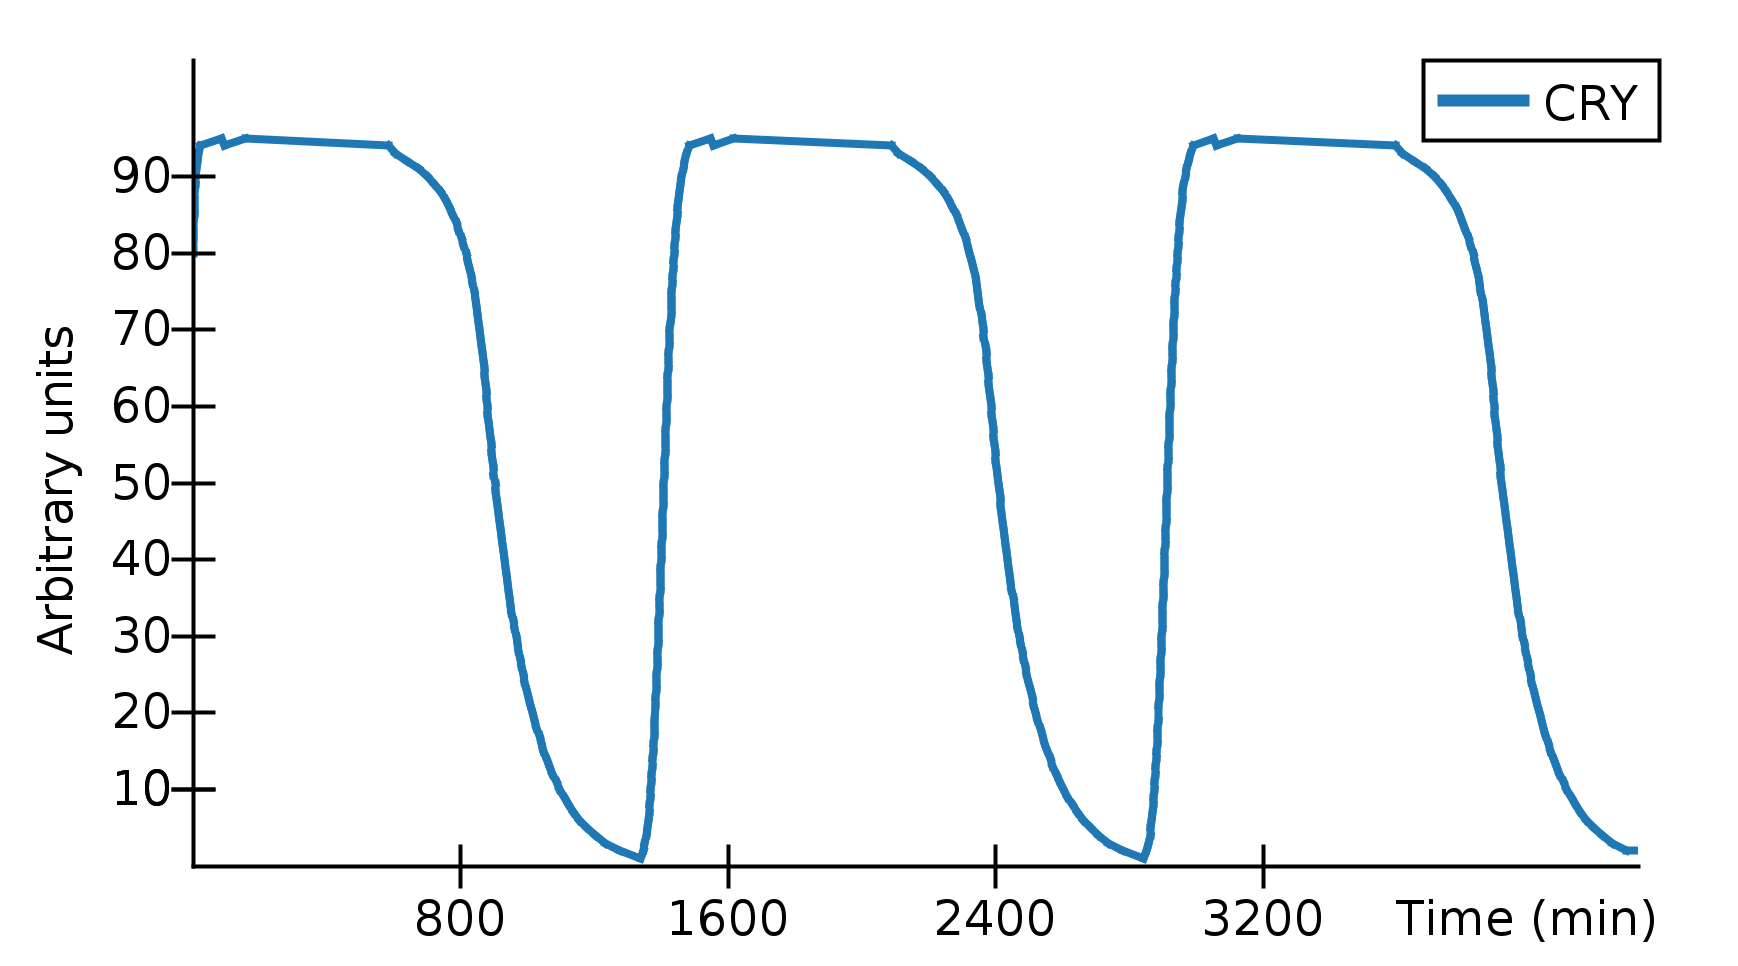
\includegraphics[width=\textwidth]{images/CRY_oscillations}\end{center}\end{minipage}}
\caption{{\bf \protect\subref{subfig:repressilator-model}} The repressilator-like subnetwork used to represent the alternation
between day and night that cause the oscillations in {\sf CRY} concentrations in the
network modeled in Section~\ref{sec:animo-drosophila}.
{\bf \protect\subref{subfig:repressilator-graph}} A graph plotting the oscillations in {\sf CRY} along
a period of three days.}\label{fig:repressilator}
\end{minipage}
\end{figure}


\subsection{ANIMO model of the Drosophila circadian clock}\label{suppl-sec:animo-drosophila}
We compared the simulation results from the ANIMO model presented in Figure~\ref{fig:drosophila-model}
with the ODE model described in~\cite{drosophila-ode-model}. The raw data coming from the
two models were aligned to have a roughly close initial point, and all amplitudes were normalized
following the procedure described in Suppl. Sect.~\ref{suppl-sec:normalization}. The results
of this comparison can be seen in Figure~\ref{suppl-fig:grafici-drosophila}.

\def\drosophilaGraphScale{0.0685}
\renewcommand*\thesubfigure{}
\begin{figure}[!htb]
\begin{minipage}{\textwidth}
  \centering
\begin{tabular}{ccc}
\subfloat[clk]{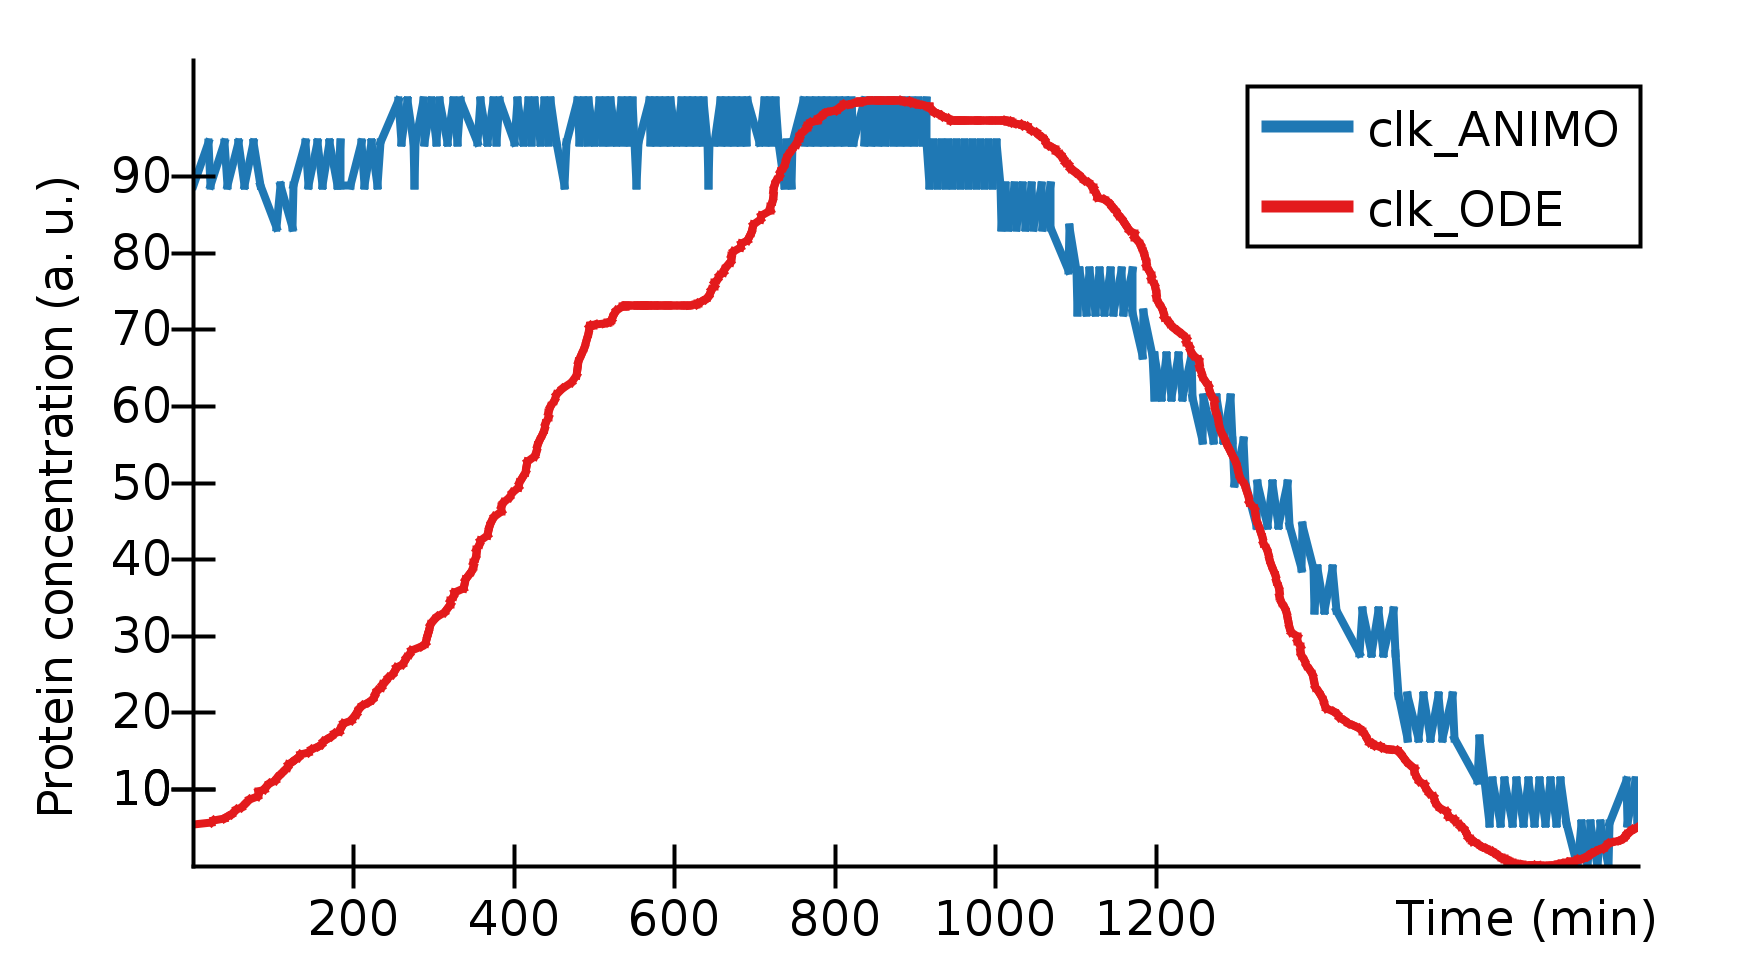
\includegraphics[scale=\drosophilaGraphScale]{images/Circadian/clk}} &
\subfloat[CLK]{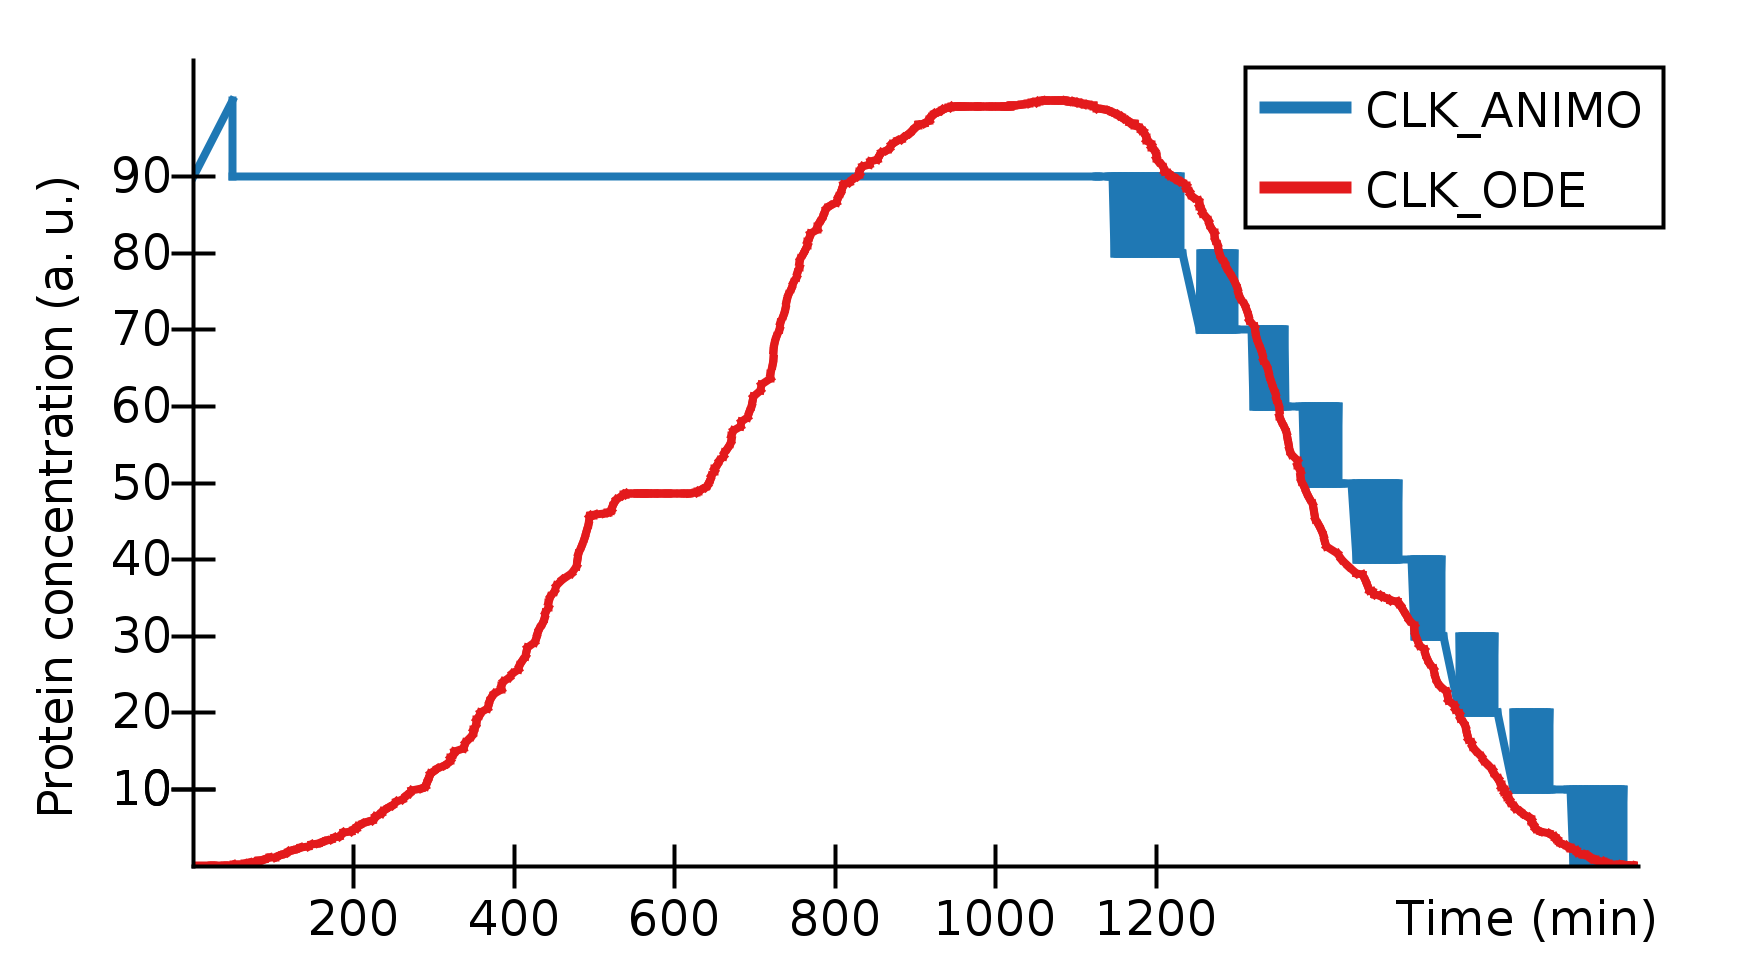
\includegraphics[scale=\drosophilaGraphScale]{images/Circadian/CLK}} &
\subfloat[CRY]{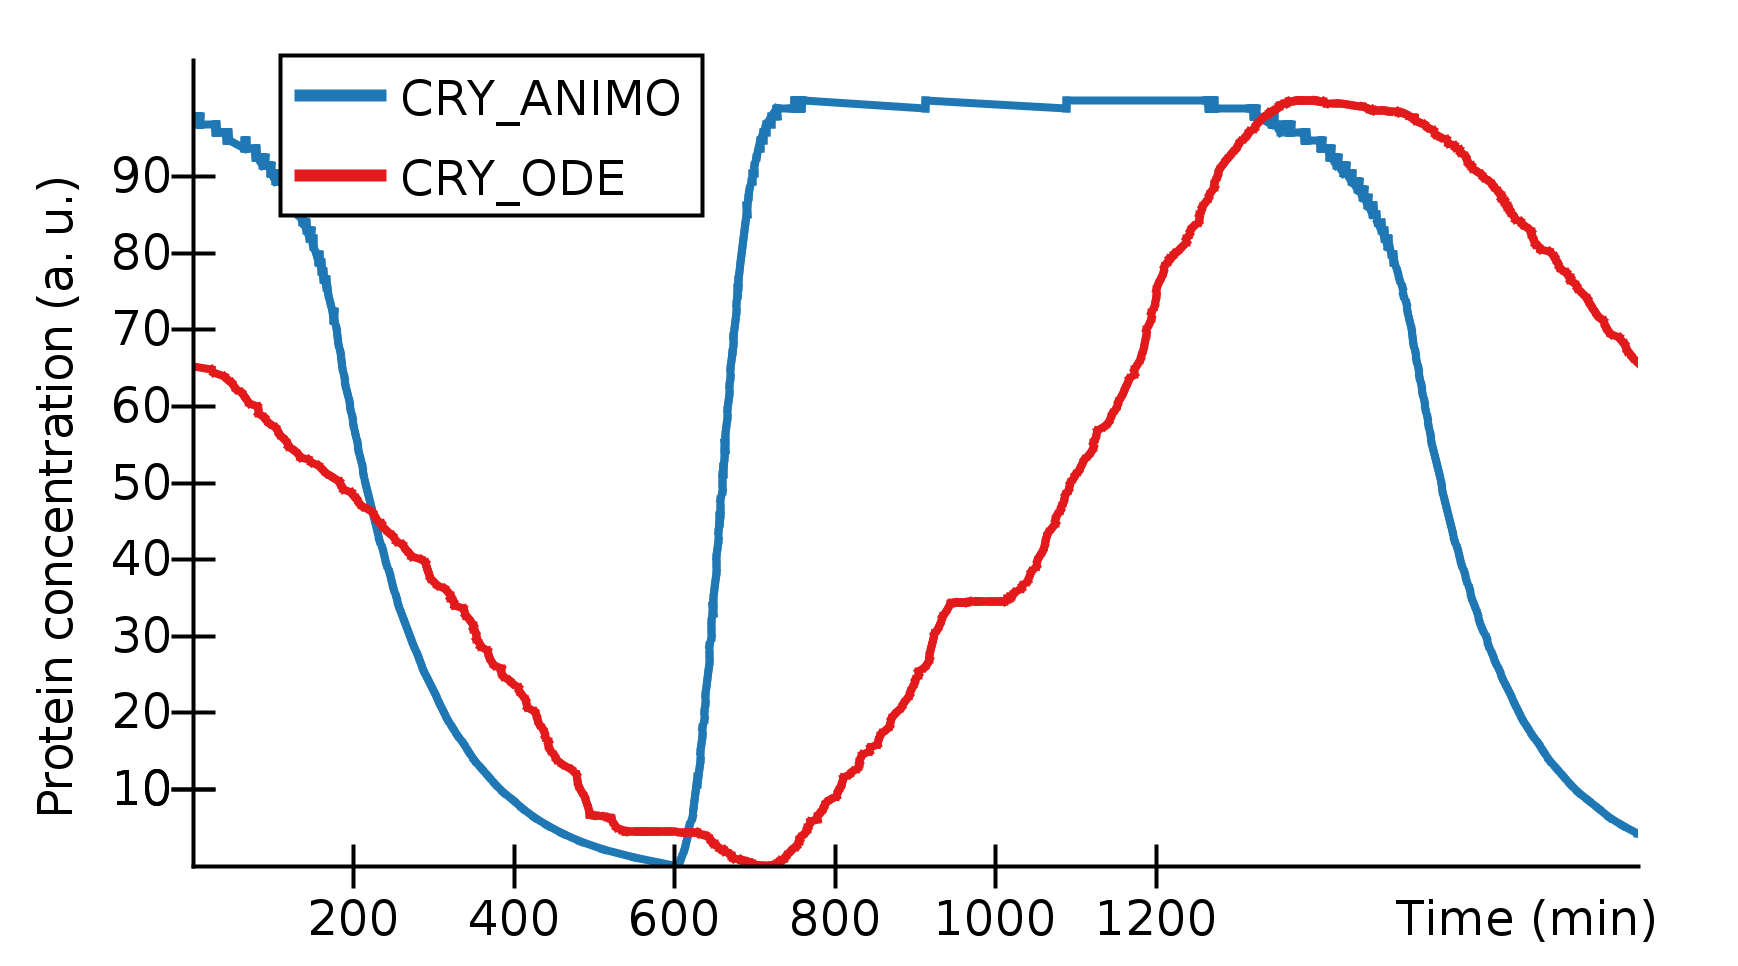
\includegraphics[scale=\drosophilaGraphScale]{images/Circadian/CRY}} \\
\subfloat[cwo]{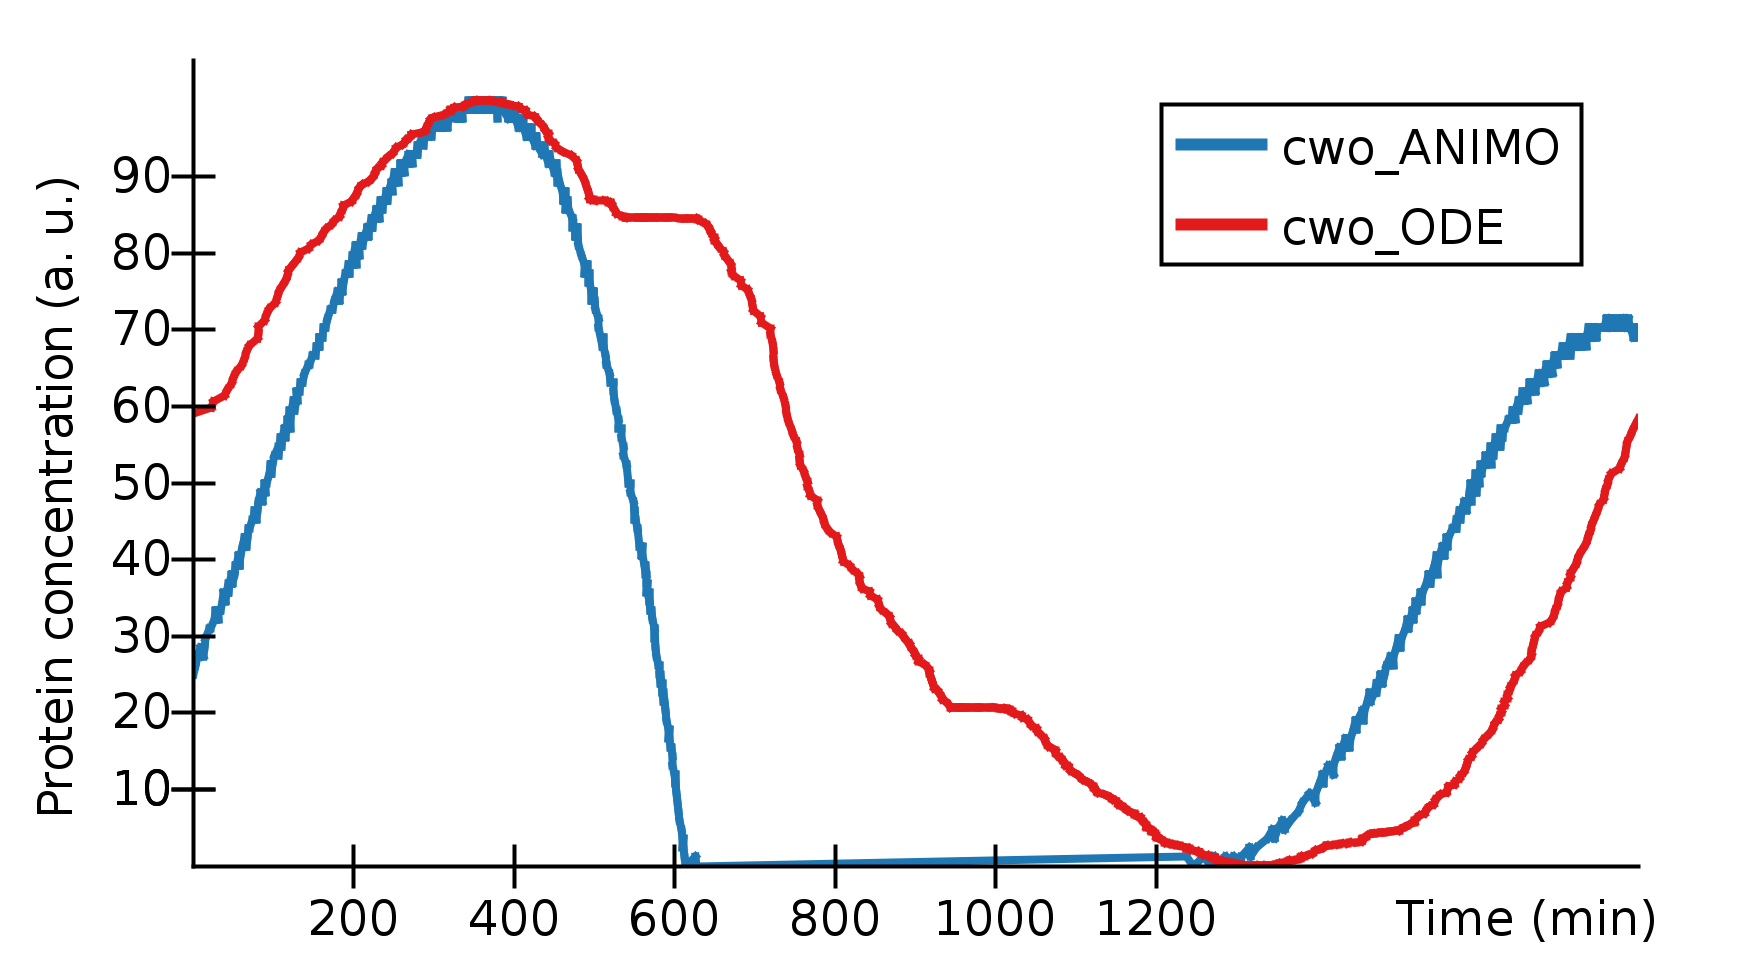
\includegraphics[scale=\drosophilaGraphScale]{images/Circadian/cwo}} &
\subfloat[CWO]{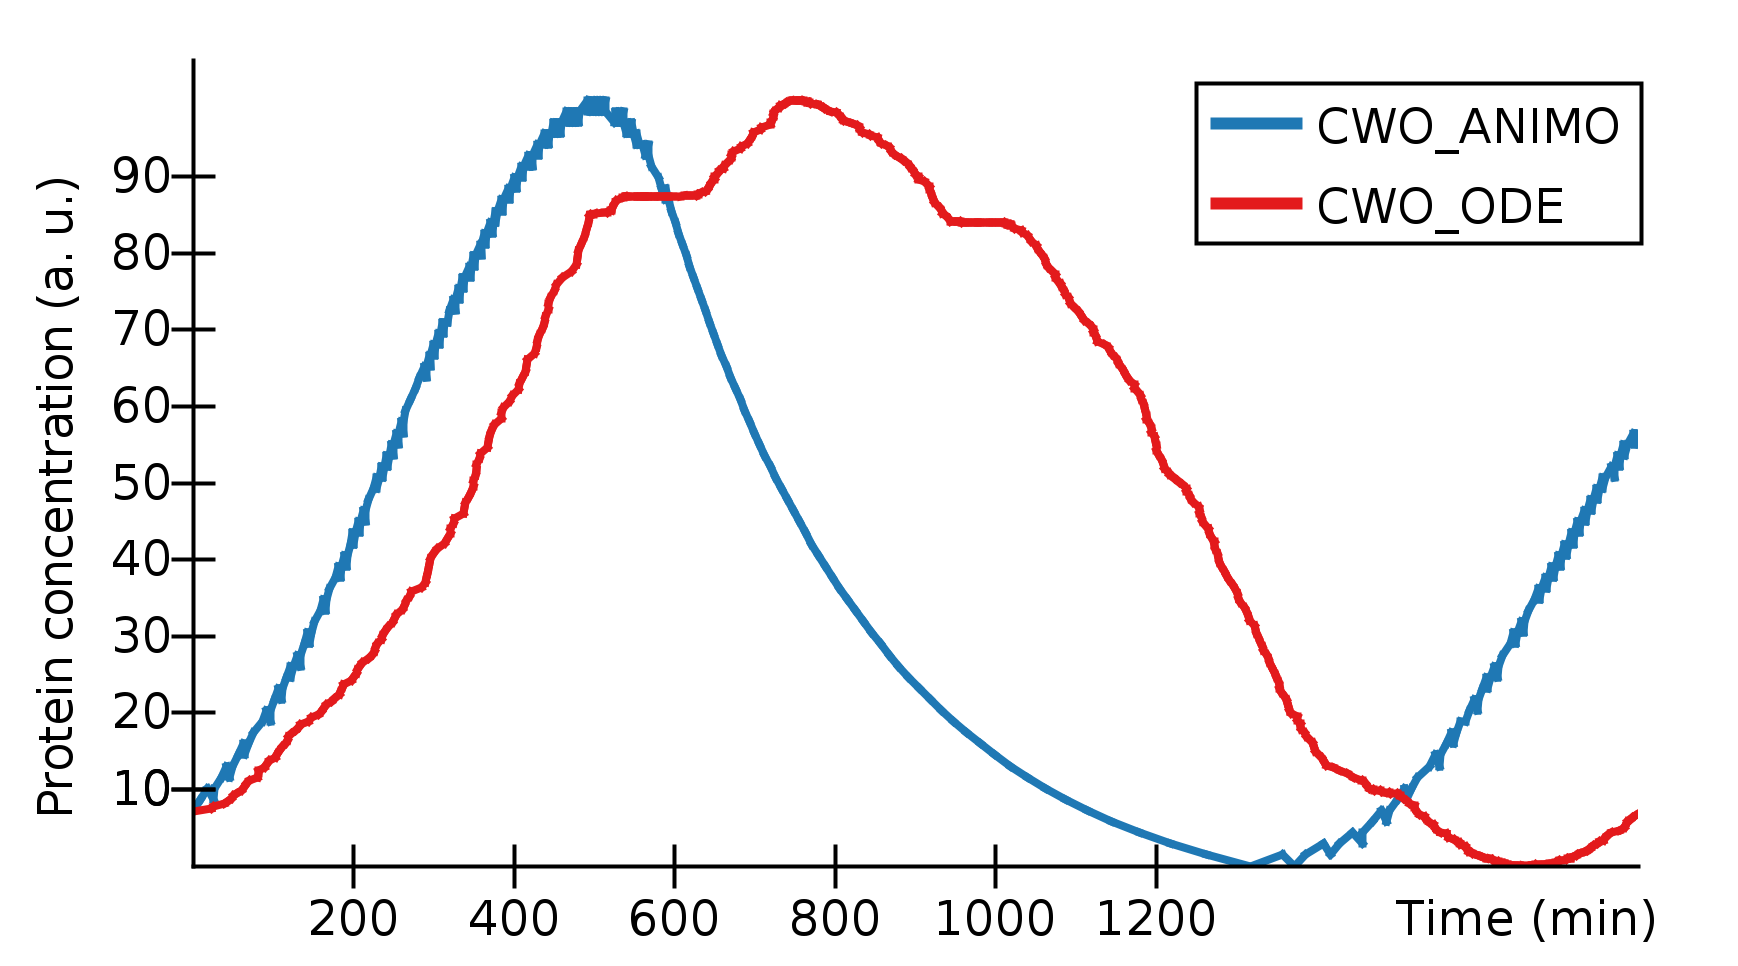
\includegraphics[scale=\drosophilaGraphScale]{images/Circadian/CWO}} &
\subfloat[CYC/CLK]{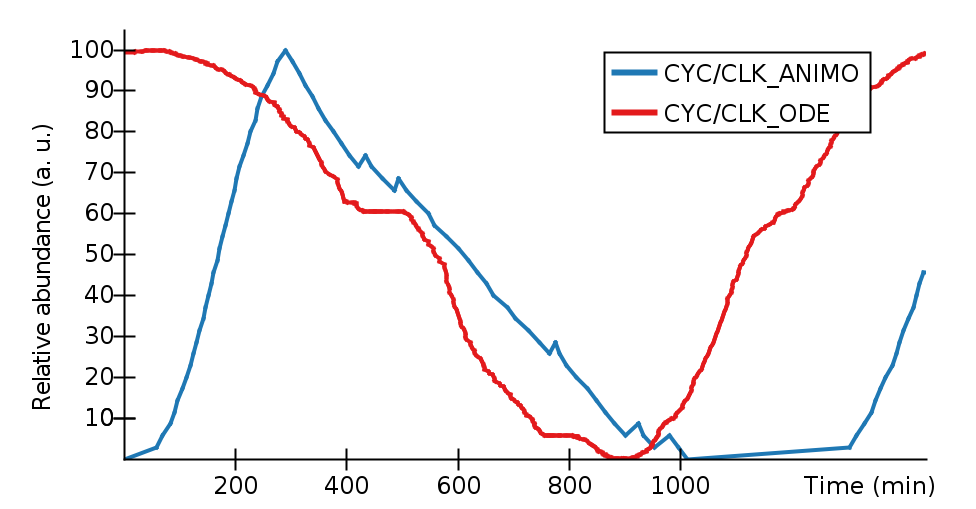
\includegraphics[scale=\drosophilaGraphScale]{images/Circadian/CYC-CLK}} \\
\subfloat[pdp1]{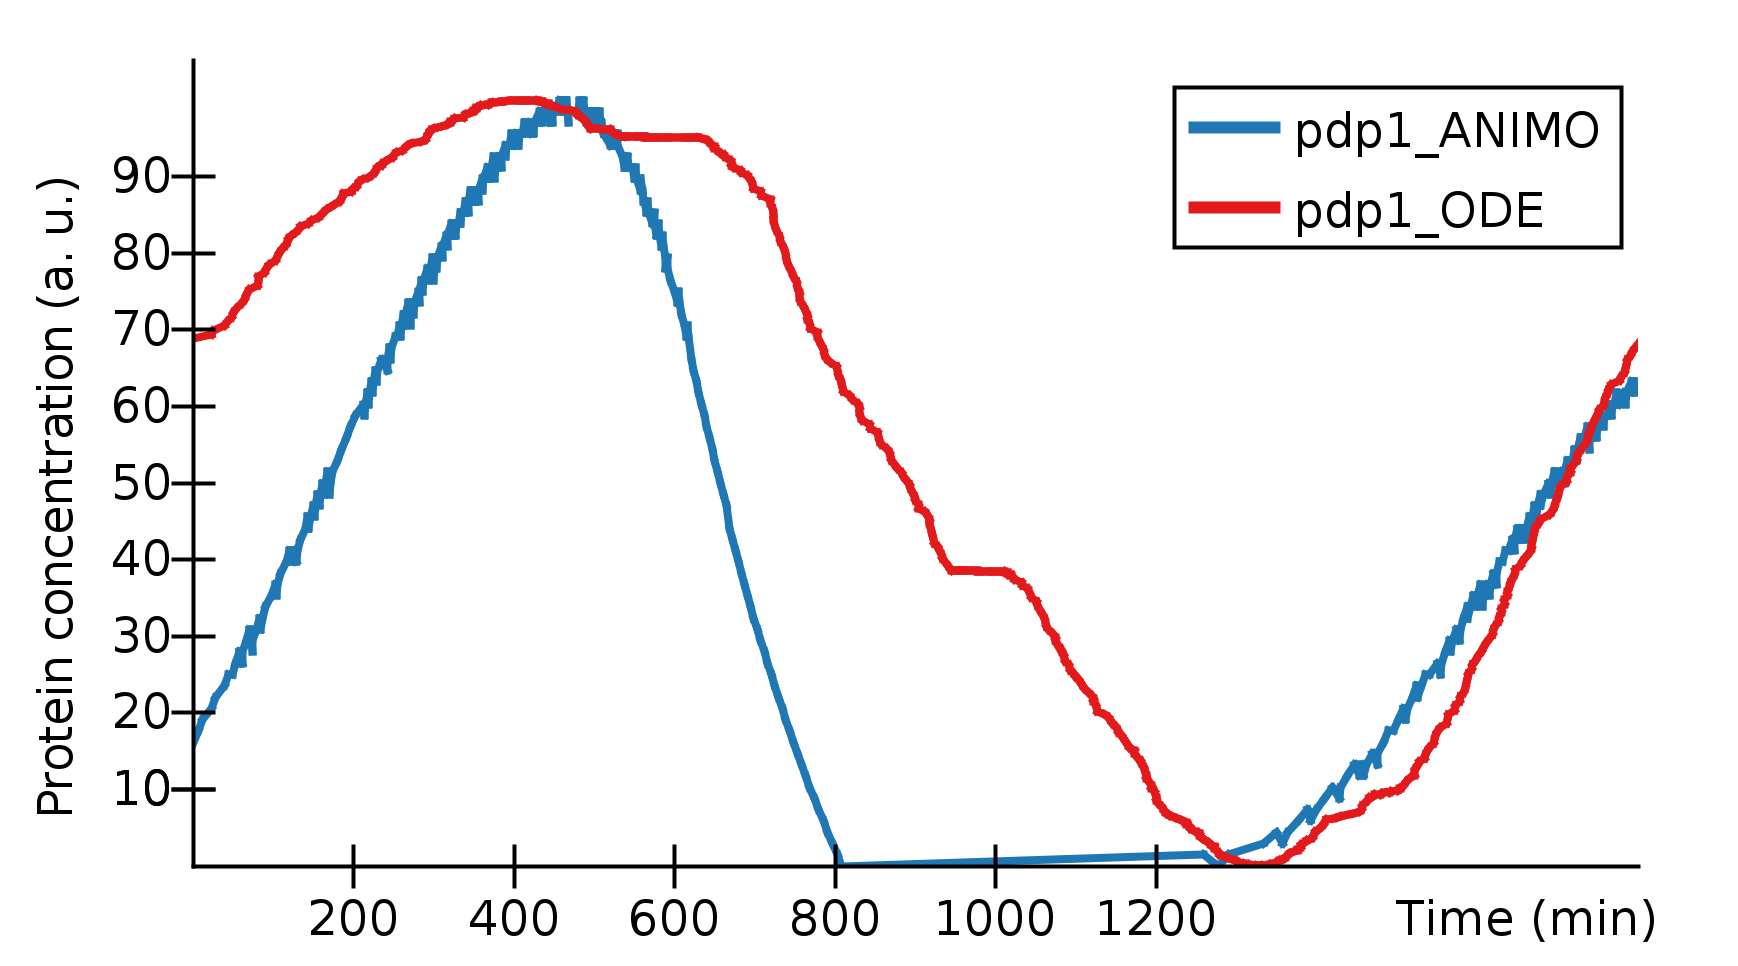
\includegraphics[scale=\drosophilaGraphScale]{images/Circadian/pdp1}} &
\subfloat[PDP1]{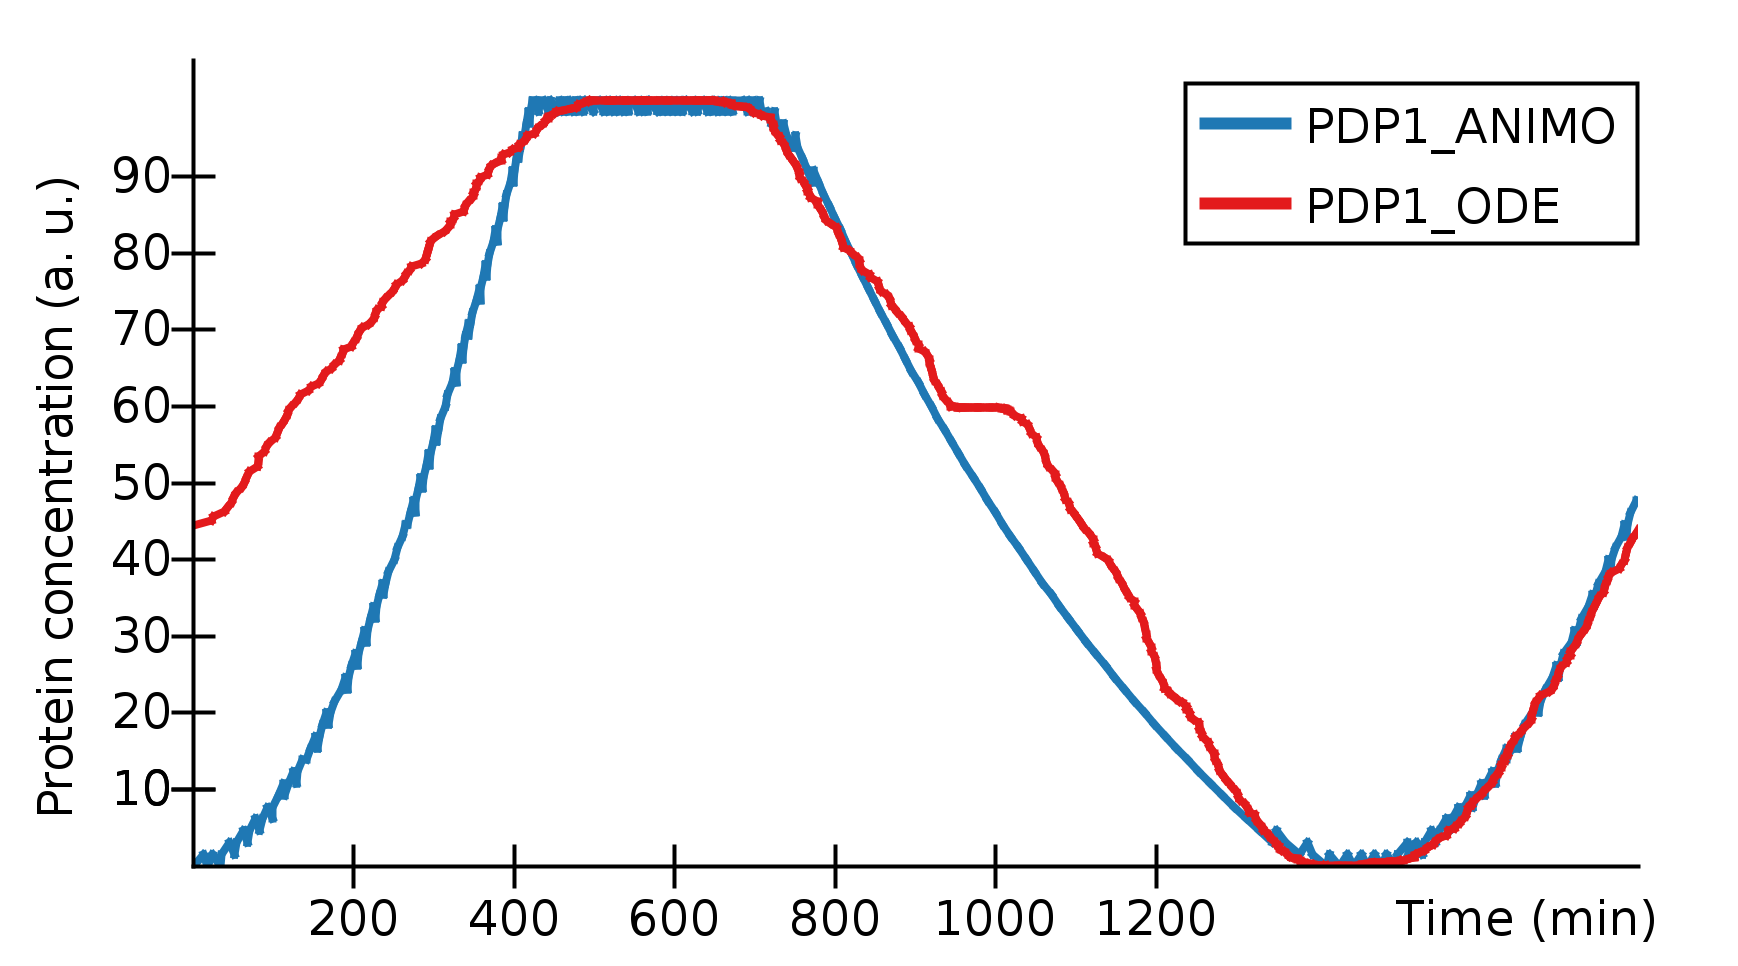
\includegraphics[scale=\drosophilaGraphScale]{images/Circadian/PDP1}} &
\subfloat[per]{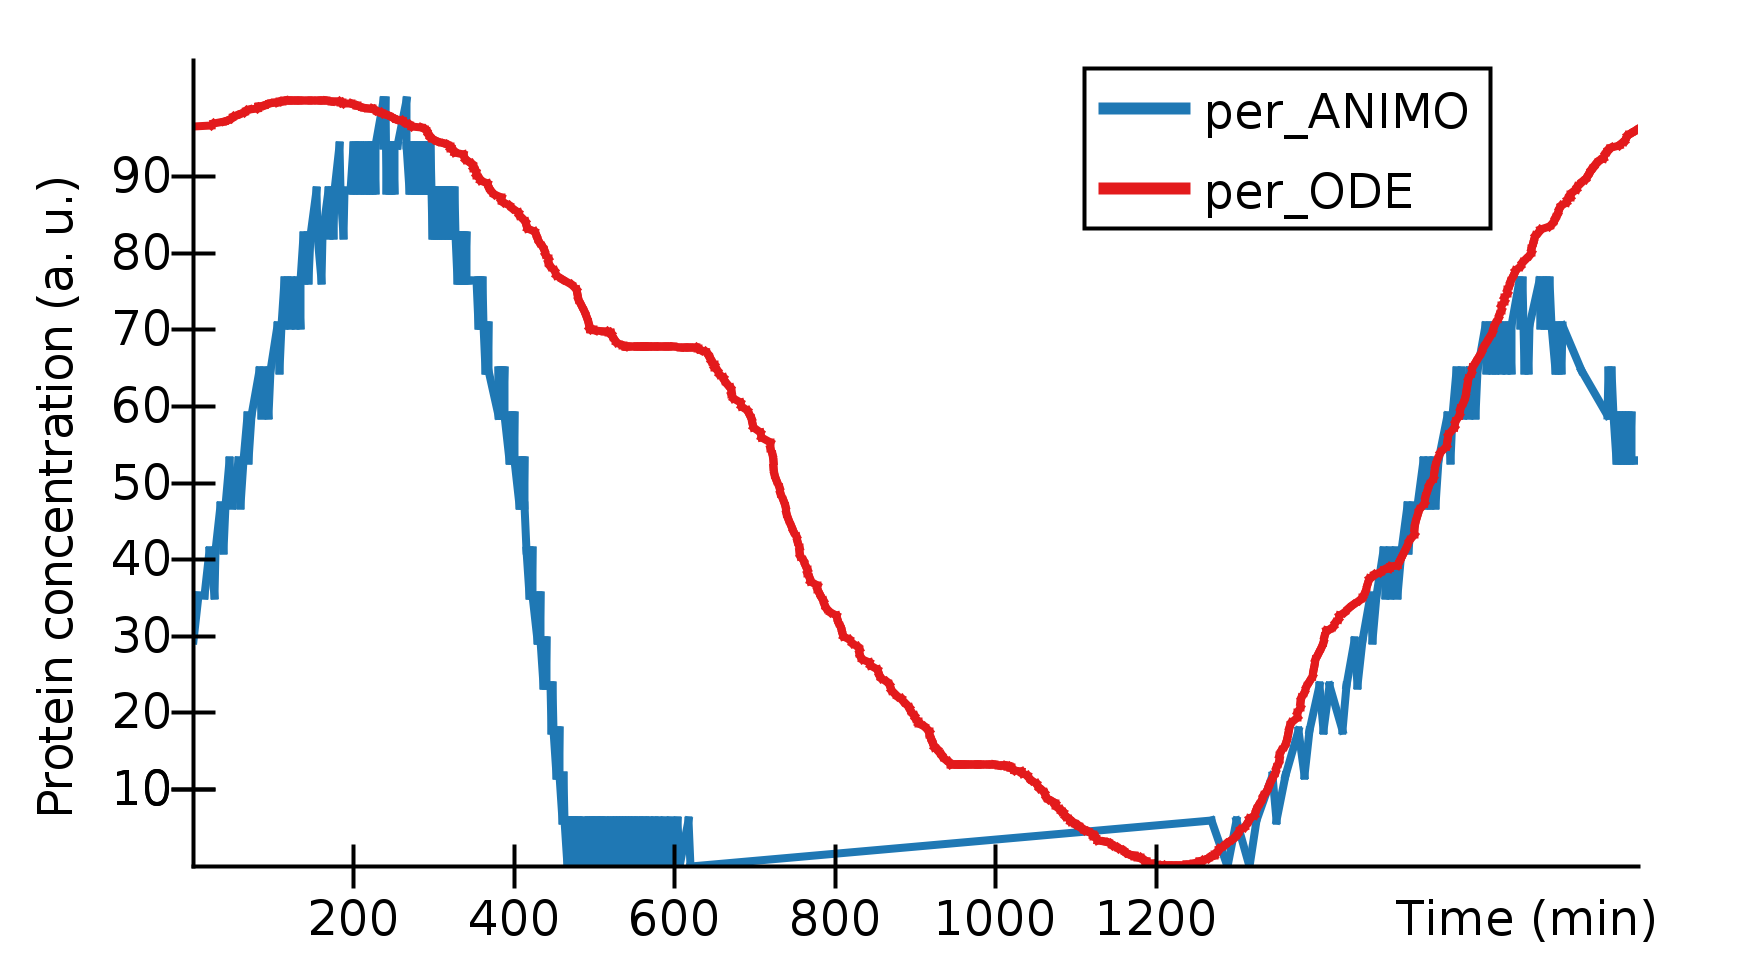
\includegraphics[scale=\drosophilaGraphScale]{images/Circadian/per}} \\
\subfloat[PER]{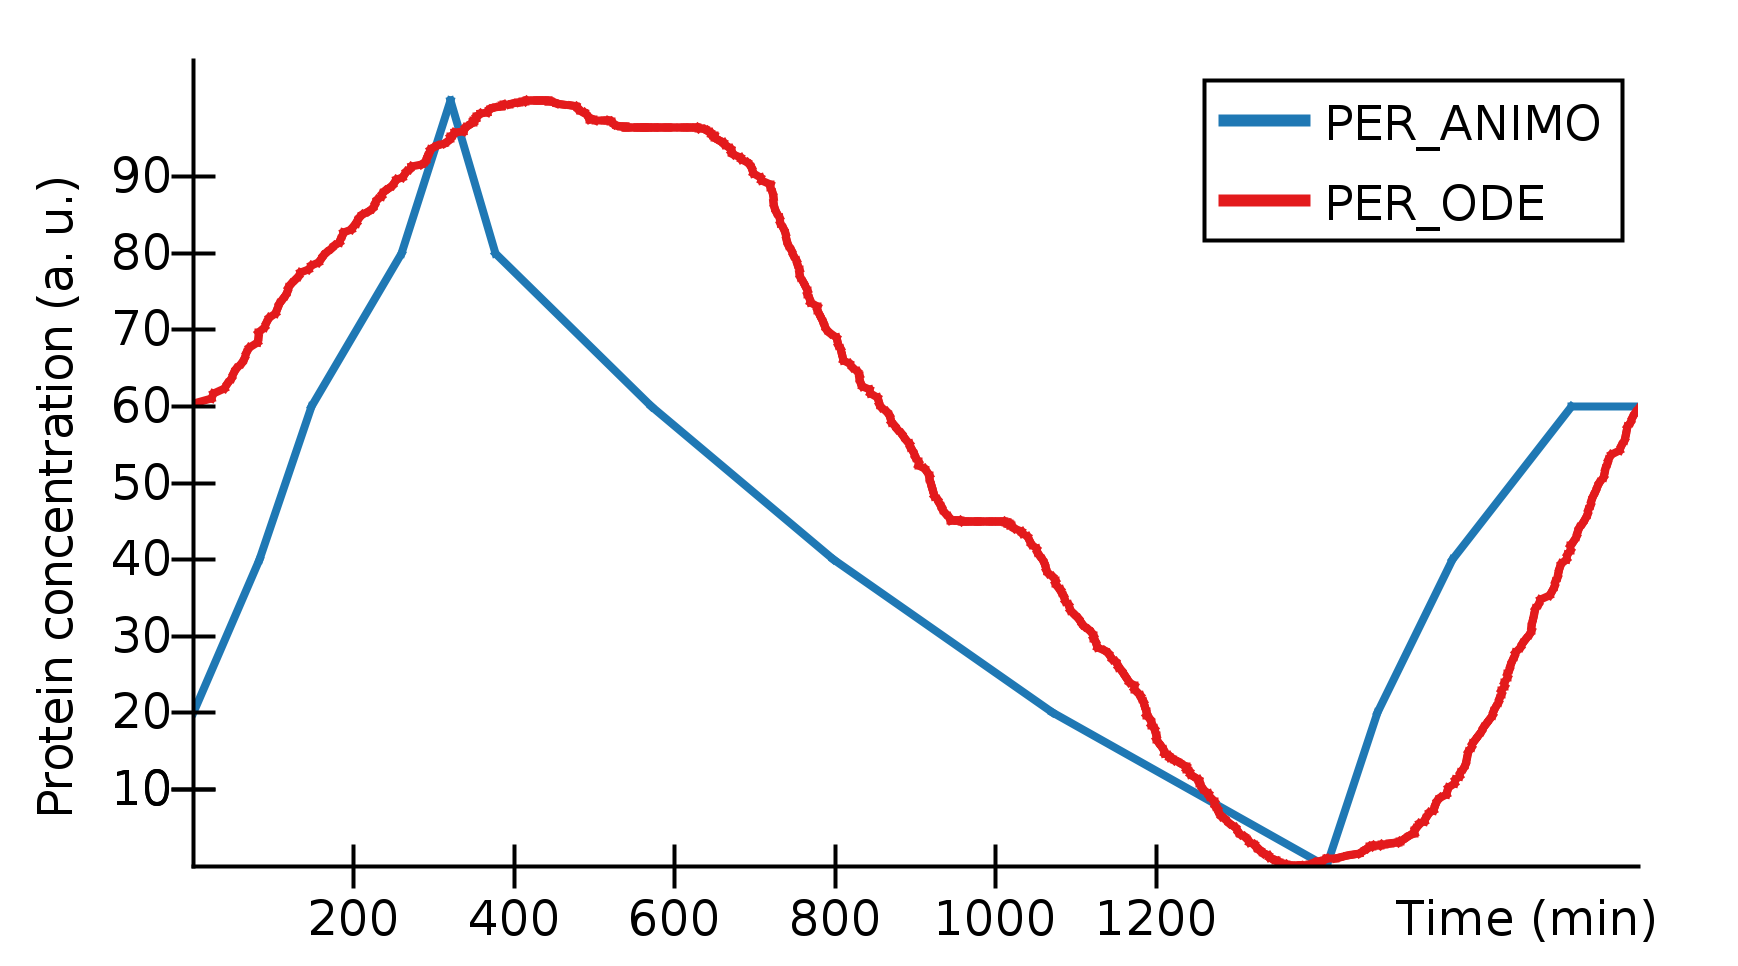
\includegraphics[scale=\drosophilaGraphScale]{images/Circadian/PER}} &
\subfloat[PER/TIM]{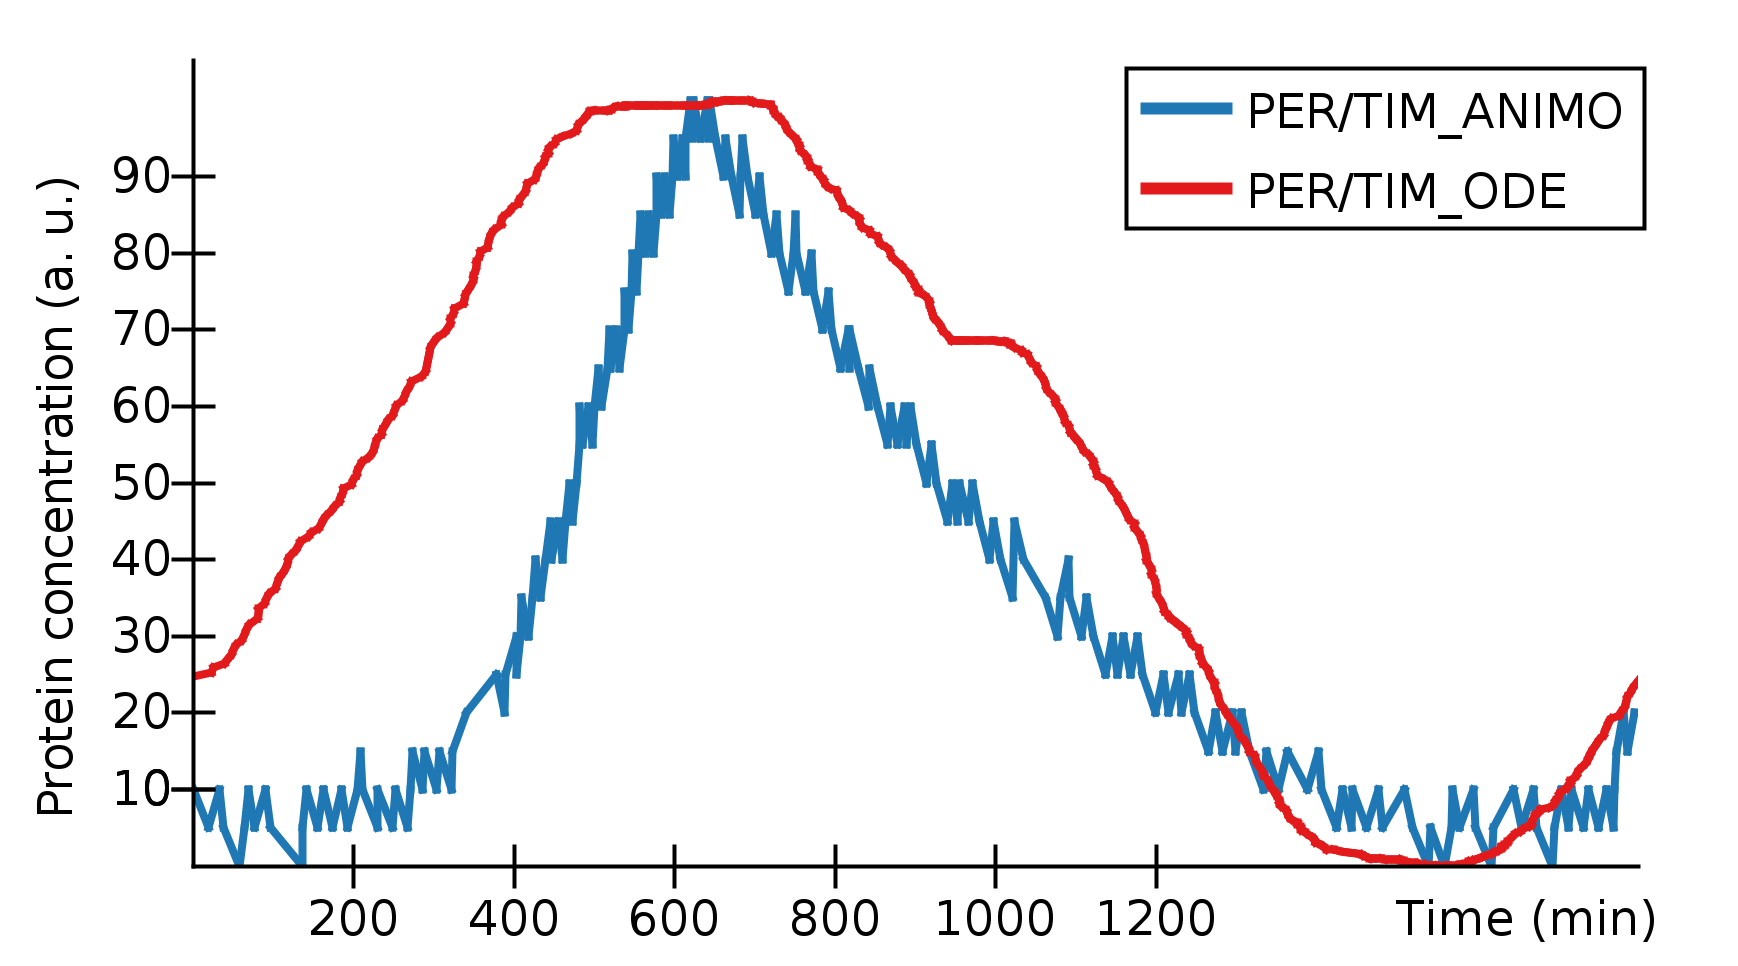
\includegraphics[scale=\drosophilaGraphScale]{images/Circadian/PER-TIM}} &
\subfloat[tim]{\includegraphics[scale=\drosophilaGraphScale]{images/Circadian/tim}} \\
\subfloat[TIM]{\includegraphics[scale=\drosophilaGraphScale]{images/Circadian/TIM}} &
\subfloat[vri]{\includegraphics[scale=\drosophilaGraphScale]{images/Circadian/vri}} &
\subfloat[VRI]{\includegraphics[scale=\drosophilaGraphScale]{images/Circadian/VRI}}
\end{tabular}
\caption{Comparing the simulation results from the ANIMO and ODE models of
\emph{Drosophila Melanogaster} circadian clock. Blue lines ({\sf \_{}ANIMO} series)
represent data from the ANIMO model in Figure~\ref{fig:drosophila-model},
while red lines ({\sf \_{}ODE} series) represent data from the ODE model in~\cite{drosophila-ode-model}.\label{suppl-fig:grafici-drosophila}}
\end{minipage}
\end{figure}

Most of the molecules represented in the two models evolve with the same period and phase.
CLK and clk in the ANIMO model have
a small oscillation range (their values change by around 10\%\ during a simulation),
so their behavior match the continuous model less precisely.
% The parameters of the ANIMO model used to represent the \emph{Drosophila Melanogaster} circadian clock in Section~\ref{sec:animo-drosophila}
% are given in Tables~\ref{tab:drosophila-model-reactants} and~\ref{tab:drosophila-model-reactions}.
%
%
%
% \begin{table}[htbp]
% \begin{minipage}{\textwidth}
% \begin{center}
% \processtable{The settings for the nodes in the model from Section~\ref{sec:animo-drosophila}.\label{tab:drosophila-model-reactants}}
% % {\begin{tabular}{llllll}%|c|c|c|c|c|c|}
% % \ \\
% % \hline\noalign{\vskip 2mm}
% %   \multirow{2}{*}{{\bfseries Name}} & {\bfseries Total act.} & {\bfseries Initial act.} & \multirow{2}{*}{{\bfseries Molecule type}} &
% % \multirow{2}{*}{{\bfseries Enabled?}} & \multirow{2}{*}{{\bfseries Plotted?}}\\
% % & {\bfseries levels} & {\bfseries level} & & & \\[2mm]
% % \hline\noalign{\vskip 2mm}
% % clk & 100 & 98 & Other & Yes & Yes \\[5mm]
% % CLK & 100 & 100 & Other & Yes & Yes \\[5mm]
% % cry & 100 & 100 & Other & Yes & Yes \\[5mm]
% % CRY & 100 & 80 & Other & Yes & Yes \\[5mm]
% % cwo & 100 & 0 & Other & Yes & Yes \\[5mm]
% % CWO & 100 & 17 & Other & Yes & Yes \\[5mm]
% % CYC & 100 & 100 & Other & Yes & No \\[5mm]
% % CYC/CLK & 100 & 0 & Other & Yes & Yes \\[5mm]
% % DBT & 100 & 100 & Other & Yes & No \\[5mm]
% % pdp1 & 100 & 0 & Other & Yes & Yes \\[5mm]
% % PDP1 & 100 & 49 & Other & Yes & Yes \\[5mm]
% % PER & 100 & 5 & Other & Yes & Yes \\[5mm]
% % per & 100 & 0 & Other & Yes & Yes \\[5mm]
% % PER/TIM-p & 100 & 46 & Other & Yes & Yes \\[5mm]
% % tim & 100 & 0 & Other & Yes & Yes \\[5mm]
% % TIM & 100 & 5 & Other & Yes & Yes \\[5mm]
% % VRI & 100 & 39 & Other & Yes & Yes \\[5mm]
% % vri & 100 & 0 & Other & Yes & Yes \\[5mm]
% % (1) & 100 & 100 & Other & Yes & No \\[5mm]
% % (2) & 100 & 69 & Other & Yes & No \\[5mm]
% % (3) & 100 & 100 & Other & Yes & No \\[5mm]
% % (4) & 100 & 0 & Other & Yes & No \\[5mm]
% % (5) & 100 & 0 & Other & Yes & No \\[5mm]
% % (6) & 100 & 100 & Other & Yes & No \\[2mm]
% % \hline
% % \end{tabular}
% {\begin{tabular}{lll||lll}
% \ \\
% \hline%\noalign{\vskip 2mm}
% & & & & & \\[-1mm]
%   \multirow{2}{*}{{\bfseries Name}} & {\bfseries Total act.} & {\bfseries Initial act.} & \multirow{2}{*}{{\bfseries Name}} &
% {\bfseries Total act.} & {\bfseries Initial act.}\\
% & {\bfseries levels} & {\bfseries level} & & {\bfseries levels} & {\bfseries level} \\[2mm]
% \hline%\noalign{\vskip 5mm}
% & & & & & \\
% clk & 100 & 98 & per & 100 & 0 \\[5mm]
% CLK & 100 & 100 & PER/TIM-p & 100 & 46 \\[5mm]
% cry & 100 & 100 & tim & 100 & 0 \\[5mm]
% CRY & 100 & 80 & TIM & 100 & 5 \\[5mm]
% cwo & 100 & 0 & VRI & 100 & 39 \\[5mm]
% CWO & 100 & 17 & vri & 100 & 0 \\[5mm]
% CYC & 100 & 100 & (1) & 100 & 100 \\[5mm]
% CYC/CLK & 100 & 0 & (2) & 100 & 69 \\[5mm]
% DBT & 100 & 100 & (3) & 100 & 100 \\[5mm]
% pdp1 & 100 & 0 & (4) & 100 & 0 \\[5mm]
% PDP1 & 100 & 49 & (5) & 100 & 0 \\[5mm]
% PER & 100 & 5 & (6) & 100 & 100 \\[2mm]
% \hline
% \end{tabular}
% }{}
% \end{center}
% \end{minipage}
% \end{table}
%
%
% \begin{table}[!ht]
% \begin{minipage}{\textwidth}
% \processtable{The settings for the edges (interactions) in the model from Section~\ref{sec:animo-drosophila}.
% $\rightarrow$ indicates activation, while $\dashv$ stands for inhibition.\label{tab:drosophila-model-reactions}}
% {\begin{tabular}{lll||lll}
% \ \\
% \hline%\noalign{\vskip 2mm}
% & & & & & \\[-1mm]
%   {\bfseries Interaction} & {\bfseries Scenario} & {\bfseries Param. value} & {\bfseries Interaction} & {\bfseries Scenario} & {\bfseries Param. value}\\[2mm]
% \hline
% & & & \\
% % \noalign{\vskip 2mm}  DBT $\rightarrow$ PER/TIM-p & 1 & 0.001 & Activation\\[5mm]
% % \noalign{\vskip 2mm}  PER/TIM-p $\dashv$ CYC/CLK & 1 & 0.32 & Inhibition\\[5mm]
% % \noalign{\vskip 2mm}  CYC $\rightarrow$ CYC/CLK & 1 & 0.02 & Activation\\[5mm]
% % \noalign{\vskip 2mm}  CLK $\rightarrow$ CYC/CLK & 1 & 0.072 & Activation\\[5mm]
% % \noalign{\vskip 2mm}  clk $\rightarrow$ CLK & 1 & 0.024 & Activation\\[5mm]
% % \noalign{\vskip 2mm}  CYC/CLK $\rightarrow$ per & 1 & 0.031 & Activation\\[5mm]
% % \noalign{\vskip 2mm}  CYC/CLK $\rightarrow$ tim & 1 & 0.015 & Activation\\[5mm]
% % \noalign{\vskip 2mm}  CYC/CLK $\rightarrow$ cwo & 1 & 0.1 & Activation\\[5mm]
% % \noalign{\vskip 2mm}  CYC/CLK $\rightarrow$ pdp1 & 1 & 0.0375 & Activation\\[5mm]
% % \noalign{\vskip 2mm}  CYC/CLK $\rightarrow$ vri & 1 & 0.03 & Activation\\[5mm]
% % \noalign{\vskip 2mm}  TIM $\rightarrow$ PER/TIM-p & 1 & 0.069 & Activation\\[5mm]
% % \noalign{\vskip 2mm}  PER $\rightarrow$ PER/TIM-p & 1 & 0.053 & Activation\\[5mm]
% % \noalign{\vskip 2mm}  per $\rightarrow$ PER & 1 & 0.0075 & Activation\\[5mm]
% % \noalign{\vskip 2mm}  cwo $\rightarrow$ CWO & 1 & 0.03 & Activation\\[5mm]
% % \noalign{\vskip 2mm}  CWO $\dashv$ cwo & 1 & 0.112 & Inhibition\\[5mm]
% % \noalign{\vskip 2mm}  vri $\rightarrow$ VRI & 1 & 0.026 & Activation\\[5mm]
% % \noalign{\vskip 2mm}  VRI $\dashv$ clk & 1 & 0.0098 & Inhibition\\[5mm]
% % \noalign{\vskip 2mm}  CWO $\dashv$ per & 1 & 0.05 & Inhibition\\[5mm]
% % \noalign{\vskip 2mm}  CWO $\dashv$ vri & 1 & 0.024 & Inhibition\\[5mm]
% % \noalign{\vskip 2mm}  CWO $\dashv$ tim & 1 & 0.02 & Inhibition\\[5mm]
% % \noalign{\vskip 2mm}  CWO $\dashv$ pdp1 & 1 & 0.0384 & Inhibition\\[5mm]
% % \noalign{\vskip 2mm}  tim $\rightarrow$ TIM & 1 & 0.056 & Activation\\[5mm]
% % \noalign{\vskip 2mm}  pdp1 $\rightarrow$ PDP1 & 1 & 0.042 & Activation\\[5mm]
% % \noalign{\vskip 2mm}  PDP1 $\rightarrow$ clk & 1 & 0.01 & Activation\\[5mm]
% % \noalign{\vskip 2mm}  cry $\rightarrow$ CRY & 2 & 0.9733 & Activation\\[5mm]
% % \noalign{\vskip 2mm}  CRY $\dashv$ TIM & 1 & 0.048 & Inhibition\\[5mm]
% % \noalign{\vskip 2mm}  cry $\dashv$ (2) & 1 & 0.10512 & Inhibition\\[5mm]
% % \noalign{\vskip 2mm}  (2) $\rightarrow$ (3) & 1 & 0.10512 & Activation\\[5mm]
% % \noalign{\vskip 2mm}  (3) $\dashv$ (4) & 1 & 0.10512 & Inhibition\\[5mm]
% % \noalign{\vskip 2mm}  (4) $\rightarrow$ (5) & 1 & 0.10512 & Activation\\[5mm]
% % \noalign{\vskip 2mm}  (5) $\dashv$ (6) & 1 & 0.10512 & Inhibition\\[5mm]
% % \noalign{\vskip 2mm}  (6) $\rightarrow$ cry & 1 & 0.10512 & Activation\\[5mm]
% % \noalign{\vskip 2mm}  (1) $\dashv$ cry & 1 & 0.0257 & Inhibition\\[5mm]
% % \noalign{\vskip 2mm}  (1) $\rightarrow$ (2) & 1 & 0.0.0518 & Activation\\[5mm]
% % \noalign{\vskip 2mm}  (1) $\dashv$ (3) & 1 & 0.0257 & Inhibition\\[5mm]
% % \noalign{\vskip 2mm}  (1) $\rightarrow$ (4) & 1 & 0.0518 & Activation\\[5mm]
% % \noalign{\vskip 2mm}  (1) $\dashv$ (5) & 1 & 0.0257 & Inhibition\\[5mm]
% % \noalign{\vskip 2mm}  (1) $\rightarrow$ (6) & 1 & 0.0518 & Activation\\[2mm]
% DBT $\rightarrow$ PER/TIM-p & 1 & 0.001 & CWO $\dashv$ tim & 1 & 0.02 \\[5mm]
% PER/TIM-p $\dashv$ CYC/CLK & 1 & 0.32 & CWO $\dashv$ pdp1 & 1 & 0.0384 \\[5mm]
% CYC $\rightarrow$ CYC/CLK & 1 & 0.02 & tim $\rightarrow$ TIM & 1 & 0.056 \\[5mm]
% CLK $\rightarrow$ CYC/CLK & 1 & 0.072 & pdp1 $\rightarrow$ PDP1 & 1 & 0.042 \\[5mm]
% clk $\rightarrow$ CLK & 1 & 0.024 & PDP1 $\rightarrow$ clk & 1 & 0.01 \\[5mm]
% CYC/CLK $\rightarrow$ per & 1 & 0.031 & cry $\rightarrow$ CRY & 2 & 0.9733 \\[5mm]
% CYC/CLK $\rightarrow$ tim & 1 & 0.015 & CRY $\dashv$ TIM & 1 & 0.048 \\[5mm]
% CYC/CLK $\rightarrow$ cwo & 1 & 0.1 & cry $\dashv$ (2) & 1 & 0.10512 \\[5mm]
% CYC/CLK $\rightarrow$ pdp1 & 1 & 0.0375 & (2) $\rightarrow$ (3) & 1 & 0.10512 \\[5mm]
% CYC/CLK $\rightarrow$ vri & 1 & 0.03 & (3) $\dashv$ (4) & 1 & 0.10512 \\[5mm]
% TIM $\rightarrow$ PER/TIM-p & 1 & 0.069 & (4) $\rightarrow$ (5) & 1 & 0.10512 \\[5mm]
% PER $\rightarrow$ PER/TIM-p & 1 & 0.053 & (5) $\dashv$ (6) & 1 & 0.10512 \\[5mm]
% per $\rightarrow$ PER & 1 & 0.0075 & (6) $\rightarrow$ cry & 1 & 0.10512 \\[5mm]
% cwo $\rightarrow$ CWO & 1 & 0.03 & (1) $\dashv$ cry & 1 & 0.0257 \\[5mm]
% CWO $\dashv$ cwo & 1 & 0.112 & (1) $\rightarrow$ (2) & 1 & 0.0.0518 \\[5mm]
% vri $\rightarrow$ VRI & 1 & 0.026 & (1) $\dashv$ (3) & 1 & 0.0257 \\[5mm]
% VRI $\dashv$ clk & 1 & 0.0098 & (1) $\rightarrow$ (4) & 1 & 0.0518 \\[5mm]
% CWO $\dashv$ per & 1 & 0.05 & (1) $\dashv$ (5) & 1 & 0.0257 \\[5mm]
% CWO $\dashv$ vri & 1 & 0.024 & (1) $\rightarrow$ (6) & 1 & 0.0518 \\[2mm]
% \hline
% \end{tabular}}{}
% \end{minipage}
% \end{table}\vspace{-2ex}


\subsection{Note on the parameters in the TNF$\alpha$-EGF model}\label{suppl:parameters-tnf-egf}
The parameters in the model in Figure~\ref{fig:large-model-complete}
have been set by fitting the model to the experimental data for conditions with 100 ng/ml TNF$\alpha$.
In the model we have set the starting level of TNF$\alpha$ at 100 out of 100 for these conditions.
This level is a dimensionless quantity that indicates the maximum activity level in the data set.
We found that setting the initial level of TNF$\alpha$ at level 8 out of 100 gave slightly better results for the
condition with 5 ng/ml TNF$\alpha$ than level 5 out of 100. We believe that this has to do with the fact that
100 ng/ml is a highly supra-physiological concentration of TNF$\alpha$, that will rapidly cause activation of all
receptors present. Fitting the model to this experimental condition may have resulted in slight deviations
in the parameter values. Nevertheless, the modeling results illustrate that building a model with basic
kinetic rate laws can give useful predictions over a range of concentrations. Figures~\ref{fig:large-model-graph3} and~\ref{fig:large-model-graph4}
show the modeling results with TNF set at 8 out of 100.



\clearpage
% \addcontentsline{toc}{section}{References}
% \begin{thebibliography}{}
% 
% \bibitem[Chaouiya et~al., 2003]{ginsim}
% Chaouiya, C., Remy, E., Moss\'{e}, B., and Thieffry, D. (2003).
% \newblock Qualitative analysis of regulatory graphs: A computational tool based
%   on a discrete formal framework.
% \newblock In Benvenuti, L., De~Santis, A., and Farina, L., editors, {\em
%   Positive Systems}, volume 294 of {\em Lecture Notes in Control and
%   Information Sciences}, pages 830--832. Springer Berlin / Heidelberg.
% 
% \bibitem[Ciocchetta et~al., 2009]{biopepa-interface}
% Ciocchetta, F., Duguid, A., Gilmore, S., Guerriero, M.~L., and Hillston, J.
%   (2009).
% \newblock {The Bio-PEPA Tool Suite}.
% \newblock {\em International Conference on Quantitative Evaluation of Systems},
%   pages 309--310.
% 
% \bibitem[de~Jong et~al., 2003]{gna}
% de~Jong, H., Geiselmann, J., Hernandez, C., and Page, M. (2003).
% \newblock {Genetic Network Analyzer: qualitative simulation of genetic
%   regulatory networks}.
% \newblock {\em Bioinformatics}, 19(3):336--344.
% 
% \bibitem[Elowitz, 2000]{repressilator}
% Elowitz, Michael~B.Leibler, S. (2000).
% \newblock A synthetic oscillatory network of transcriptional regulators.
% \newblock {\em Nature}, 403(6767):335.
% 
% \bibitem[Fathallah-Shaykh et~al., 2009]{drosophila-ode-model}
% Fathallah-Shaykh, H.~M., Bona, J.~L., and Kadener, S. (2009).
% \newblock Mathematical model of the drosophila circadian clock: Loop regulation
%   and transcriptional integration.
% \newblock {\em Biophysical Journal}, 97(9):2399 -- 2408.
% 
% \bibitem[Janes et~al., 2006]{pathway-autocrine}
% Janes, K.~A., Gaudet, S., Albeck, J.~G., Nielsen, U.~B., Lauffenburger, D.~A.,
%   and Sorger, P.~K. (2006).
% \newblock The response of human epithelial cells to {TNF} involves an inducible
%   autocrine cascade.
% \newblock {\em Cell}, 124(6):1225--1239.
% 
% \bibitem[Kadener et~al., 2007]{drosophila-cry-data}
% Kadener, S., Stoleru, D., McDonald, M., Nawathean, P., and Rosbash, M. (2007).
% \newblock Clockwork orange is a transcriptional repressor and a new drosophila
%   circadian pacemaker component.
% \newblock {\em Genes \& Development}, 21(13):1675--1686.
% 
% \bibitem[Killcoyne et~al., 2009]{cytoscape}
% Killcoyne, S., Carter, G.~W., Smith, J., and Boyle, J. (2009).
% \newblock {Cytoscape: a community-based framework for network modeling.}
% \newblock {\em Methods in molecular biology (Clifton, N.J.)}, 563:219--239.
% 
% \bibitem[Larsen et~al., 1997]{uppaal}
% Larsen, K.~G., Pettersson, P., and Yi, W. (1997).
% \newblock {UPPAAL} in a nutshell.
% \newblock {\em International Journal on Software Tools for Technology Transfer
%   (STTT)}, 1:134--152.
% 
% \bibitem[Mendes et~al., 2009]{copasi}
% Mendes, P., Hoops, S., Sahle, S., Gauges, R., Dada, J., and Kummer, U. (2009).
% \newblock {Computational modeling of biochemical networks using COPASI systems
%   biology}.
% \newblock volume 500 of {\em Methods in Molecular Biology}, chapter~2, pages
%   17--59. Humana Press, Totowa, NJ.
% 
% \bibitem[Nagasaki et~al., 2011]{cell-illustrator}
% Nagasaki, M., Saito, A., Jeong, E., Li, C., Kojima, K., Ikeda, E., and Miyano,
%   S. (2011).
% \newblock Cell illustrator 4.0: a computational platform for systems biology.
% \newblock {\em Stud Health Technol Inform}, 162:160--81.
% 
% \bibitem[Schivo et~al., 2012]{animo-ieee}
% Schivo, S., Scholma, J., Wanders, B., {Urquidi Camacho}, R.~A., van~der Vet,
%   P.~E., Karperien, M., Langerak, R., van~de Pol, J., and Post, J.~N. (2012).
% \newblock Modelling biological pathway dynamics with {Timed Automata}.
% \newblock {\em IEEE Journal of Biomedical and Health Informatics}. IEEE Engineering
%   in Medicine and Biology Society.
% 
% \end{thebibliography}





\clearpage

\section{Supplementary figures}\label{sec:supplementary-figures}
\addcontentsline{toc}{section}{Supplementary figures}


\begin{figure}[htpb]
\begin{minipage}{\textwidth}
\centering
  \includegraphics[width=.7\textwidth]{images/large_network_tnfa2}
\caption{The model for the TNF$\alpha$ pathway in isolation. Node colors represent the activity level of the
corresponding modeled reactants at time $t = 10$ minutes after a stimulation of 100 ng/ml TNF$\alpha$.}\label{fig:large-model-tnf}
\end{minipage}
\end{figure}

\begin{figure}[!tpb]
\begin{minipage}{\textwidth}
\centering
  \includegraphics[width=.7\textwidth]{images/large_network_egf3}
\caption{The model for the EGF pathway in isolation. Node colors represent the
activity level of the corresponding modeled reactants at time $t = 5$ minutes after
a stimulation of 100 ng/ml EGF.}\label{fig:large-model-egf}
\end{minipage}
\end{figure}

\def\largeModelScale{0.18}%0.15}%0.155}%0.27}
\def\legendScalaColori{0.21}%0.18}%0.21}
\def\legendScalaForme{0.21}%0.18}%0.21}
\def\scalaGrafici{0.0709}%0.13}
\begin{figure}[!tpb]
\begin{minipage}{\textwidth}
\centering
  \subfloat{\includegraphics[width=\textwidth]{images/large_network_hypotheses7}}\\
\subfloat{\includegraphics[scale=\legendScalaColori]{images/legenda_forme}} \subfloat{\includegraphics[scale=\legendScalaForme]{images/legenda_colori}}
\caption{The merged model for the TNF$\alpha$-EGF pathway in which
the two hypotheses are highlighted. The first hypothesis is the dependence IL-1$\alpha$ expression on the
combined activity of ERK and JNK1. The second hypothesis assumes an as yet unidentified protein (Hyp2) to link EGFR to MEKK1.
Node colors represent initial activity levels.}\label{fig:large-model-hypotheses}
\end{minipage}
\end{figure}


\renewcommand*\thesubfigure{}
\begin{figure}[!tpb]
\begin{minipage}{\textwidth}
\begin{tabularx}{\textwidth}{XXX}
\subfloat[MK2 (2 hours)]{\includegraphics[width=0.29\textwidth]{images/TNFa100/MK2}} &
\subfloat[JNK1 (2 hours)]{\includegraphics[width=0.29\textwidth]{images/TNFa100/JNK1}} &
\subfloat[IKK (2 hours)]{\includegraphics[width=0.29\textwidth]{images/TNFa100/IKK_120}} \\
\subfloat[IKK (24 hours)]{\includegraphics[width=0.29\textwidth]{images/TNFa100/IKK_1440}} &
\subfloat[caspase-8 (24 hours)]{\includegraphics[width=0.29\textwidth]{images/TNFa100/casp8}} &
\subfloat[caspase-3 (24 hours)]{\includegraphics[width=0.29\textwidth]{images/TNFa100/casp3}} \\
\subfloat[MEK (2 hours)]{\includegraphics[width=0.29\textwidth]{images/TNFa100/MEK}} &
\subfloat[ERK (2 hours)]{\includegraphics[width=0.29\textwidth]{images/TNFa100/ERK}} &
\subfloat[Akt (24 hours)]{\includegraphics[width=0.29\textwidth]{images/TNFa100/Akt}} \\
\subfloat[IRS-1(S) (2 hours)]{\includegraphics[width=0.29\textwidth]{images/TNFa100/IRS1s_120}} &
\subfloat[IRS-1(Y) (2 hours)]{\includegraphics[width=0.29\textwidth]{images/TNFa100/IRS1y_120}} &
\subfloat[FKHR (12 hours)]{\includegraphics[width=0.29\textwidth]{images/TNFa100/FKHR_720}}
\end{tabularx}
\caption{Comparison between the ANIMO model in Figure~\ref{fig:large-model-complete} and experimental data. Treatment condition: 100 ng/ml TNF$\alpha$.
In order to ease the comparison for earlier responses, the time span for those cases is less than 24 hours.}\label{fig:differences1}
\end{minipage}
\end{figure}


\begin{figure}[!tpb]
\begin{minipage}{\textwidth}
\begin{tabularx}{\textwidth}{XXX}
\subfloat[MK2 (2 hours)]{\includegraphics[width=0.29\textwidth]{images/EGF100/MK2}} &
\subfloat[JNK1 (2 hours)]{\includegraphics[width=0.29\textwidth]{images/EGF100/JNK1}} &
\subfloat[IKK (24 hours)]{\includegraphics[width=0.29\textwidth]{images/EGF100/IKK}} \\
\subfloat[caspase-8 (24 hours)]{\includegraphics[width=0.29\textwidth]{images/EGF100/casp8}} &
\subfloat[caspase-3 (24 hours)]{\includegraphics[width=0.29\textwidth]{images/EGF100/casp3}} &
\subfloat[MEK (2 hours)]{\includegraphics[width=0.29\textwidth]{images/EGF100/MEK}} \\
\subfloat[ERK (2 hours)]{\includegraphics[width=0.29\textwidth]{images/EGF100/ERK}} &
\subfloat[Akt (2 hours)]{\includegraphics[width=0.29\textwidth]{images/EGF100/Akt_120}} &
\subfloat[Akt (24 hours)]{\includegraphics[width=0.29\textwidth]{images/EGF100/Akt_1440}} \\
\subfloat[IRS-1(S) (2 hours)]{\includegraphics[width=0.29\textwidth]{images/EGF100/IRS1s_120}} &
\subfloat[IRS-1(Y) (2 hours)]{\includegraphics[width=0.29\textwidth]{images/EGF100/IRS1y_120}} &
\subfloat[IRS-1(Y) (12 hours)]{\includegraphics[width=0.29\textwidth]{images/EGF100/IRS1y_720}} \\
\subfloat[FKHR (2 hours)]{\includegraphics[width=0.29\textwidth]{images/EGF100/FKHR_120}} &
\subfloat[FKHR (12 hours)]{\includegraphics[width=0.29\textwidth]{images/EGF100/FKHR_720}}
\end{tabularx}
\caption{Comparison between the ANIMO model in Figure~\ref{fig:large-model-complete} and experimental data. Treatment condition: 100 ng/ml EGF.
In order to ease the comparison for earlier responses, the time span for those cases is less than 24 hours.}\label{fig:differences2}
\end{minipage}
\end{figure}


\begin{figure}[!tpb]
\begin{minipage}{\textwidth}
\begin{tabularx}{\textwidth}{XXX}
\subfloat[MK2 (2 hours)]{\includegraphics[width=0.29\textwidth]{images/TNFa100_EGF100/MK2}} &
\subfloat[JNK1 (2 hours)]{\includegraphics[width=0.29\textwidth]{images/TNFa100_EGF100/JNK1}} &
\subfloat[IKK (24 hours)]{\includegraphics[width=0.29\textwidth]{images/TNFa100_EGF100/IKK}} \\
\subfloat[caspase-8 (24 hours)]{\includegraphics[width=0.29\textwidth]{images/TNFa100_EGF100/casp8}} &
\subfloat[caspase-3 (24 hours)]{\includegraphics[width=0.29\textwidth]{images/TNFa100_EGF100/casp3}} &
\subfloat[MEK (2 hours)]{\includegraphics[width=0.29\textwidth]{images/TNFa100_EGF100/MEK}} \\
\subfloat[ERK (2 hours)]{\includegraphics[width=0.29\textwidth]{images/TNFa100_EGF100/ERK}} &
\subfloat[Akt (2 hours)]{\includegraphics[width=0.29\textwidth]{images/TNFa100_EGF100/Akt}} &
\subfloat[IRS-1(S) (2 hours)]{\includegraphics[width=0.29\textwidth]{images/TNFa100_EGF100/IRS1s_120}} \\
\subfloat[IRS-1(S) (12 hours)]{\includegraphics[width=0.29\textwidth]{images/TNFa100_EGF100/IRS1s_720}} &
\subfloat[IRS-1(Y) (2 hours)]{\includegraphics[width=0.29\textwidth]{images/TNFa100_EGF100/IRS1y}} &
\subfloat[FKHR (4 hours)]{\includegraphics[width=0.29\textwidth]{images/TNFa100_EGF100/FKHR_240}}
\end{tabularx}
\caption{Comparison between the ANIMO model in Figure~\ref{fig:large-model-complete} and experimental data. Treatment condition: 100 ng/ml TNF$\alpha$ + 100 ng/ml EGF.
In order to ease the comparison for earlier responses, the time span for those cases is less than 24 hours.}\label{fig:differences3}
\end{minipage}
\end{figure}


\end{document}
